\documentclass[a4paper]{book}
\usepackage{a4wide}
\usepackage{makeidx}
\usepackage{fancyhdr}
\usepackage{graphicx}
\usepackage{multicol}
\usepackage{float}
\usepackage{textcomp}
\usepackage{alltt}
\usepackage{doxygen}
\makeindex
\setcounter{tocdepth}{1}
\renewcommand{\footrulewidth}{0.4pt}
\begin{document}
\begin{titlepage}
\vspace*{7cm}
\begin{center}
{\Large Reference Manual}\\
\vspace*{1cm}
{\large Generated by Doxygen 1.4.7}\\
\vspace*{0.5cm}
{\small Mon Jul 14 09:35:52 2014}\\
\end{center}
\end{titlepage}
\clearemptydoublepage
\pagenumbering{roman}
\tableofcontents
\clearemptydoublepage
\pagenumbering{arabic}
\chapter{Hierarchical Index}
\section{Class Hierarchy}
This inheritance list is sorted roughly, but not completely, alphabetically:\begin{CompactList}
\item \contentsline{section}{CAngle}{\pageref{classCAngle}}{}
\item \contentsline{section}{CAngle\-Dist}{\pageref{classCAngleDist}}{}
\item \contentsline{section}{CChart}{\pageref{classCChart}}{}
\item \contentsline{section}{CEvap}{\pageref{classCEvap}}{}
\item \contentsline{section}{CFus}{\pageref{classCFus}}{}
\item \contentsline{section}{CGdr}{\pageref{classCGdr}}{}
\item \contentsline{section}{CHistory}{\pageref{classCHistory}}{}
\item \contentsline{section}{CLevel\-Density}{\pageref{classCLevelDensity}}{}
\item \contentsline{section}{CMass}{\pageref{classCMass}}{}
\item \contentsline{section}{CNuclide}{\pageref{classCNuclide}}{}
\begin{CompactList}
\item \contentsline{section}{CLight\-P}{\pageref{classCLightP}}{}
\item \contentsline{section}{CNucleus}{\pageref{classCNucleus}}{}
\end{CompactList}
\item \contentsline{section}{CRandom}{\pageref{classCRandom}}{}
\item \contentsline{section}{CRun}{\pageref{classCRun}}{}
\item \contentsline{section}{CRun\-Thick}{\pageref{classCRunThick}}{}
\item \contentsline{section}{CScission}{\pageref{classCScission}}{}
\item \contentsline{section}{CSig\-Bar\-Dist}{\pageref{classCSigBarDist}}{}
\item \contentsline{section}{CSig\-Charged}{\pageref{classCSigCharged}}{}
\item \contentsline{section}{CTl\-Array}{\pageref{classCTlArray}}{}
\item \contentsline{section}{CTl\-Bar\-Dist}{\pageref{classCTlBarDist}}{}
\item \contentsline{section}{CWeight}{\pageref{classCWeight}}{}
\begin{CompactList}
\item \contentsline{section}{CNucleus}{\pageref{classCNucleus}}{}
\end{CompactList}
\item \contentsline{section}{CYrast}{\pageref{classCYrast}}{}
\item \contentsline{section}{Lshape}{\pageref{structLshape}}{}
\item \contentsline{section}{SAng\-Tl}{\pageref{structSAngTl}}{}
\item \contentsline{section}{SDecay}{\pageref{structSDecay}}{}
\item \contentsline{section}{SIsotope}{\pageref{structSIsotope}}{}
\item \contentsline{section}{SStore}{\pageref{structSStore}}{}
\item \contentsline{section}{SStore\-Chan}{\pageref{structSStoreChan}}{}
\item \contentsline{section}{SStore\-Evap}{\pageref{structSStoreEvap}}{}
\item \contentsline{section}{SStore\-Sub}{\pageref{structSStoreSub}}{}
\item \contentsline{section}{SZcoef}{\pageref{structSZcoef}}{}
\end{CompactList}

\chapter{Class Index}
\section{Class List}
Here are the classes, structs, unions and interfaces with brief descriptions:\begin{CompactList}
\item\contentsline{section}{\bf{CAngle} (Polar angles )}{\pageref{classCAngle}}{}
\item\contentsline{section}{\bf{CAngle\-Dist} (Angular distributions )}{\pageref{classCAngleDist}}{}
\item\contentsline{section}{\bf{CChart} (Defines accessable region of chart of nuclides )}{\pageref{classCChart}}{}
\item\contentsline{section}{\bf{CEvap} (Stores info for light particle evaporation )}{\pageref{classCEvap}}{}
\item\contentsline{section}{\bf{CFus} (Fusion xsection, Bass model, excitation energy in fusion )}{\pageref{classCFus}}{}
\item\contentsline{section}{\bf{CGdr} (User-defined GDR line shape )}{\pageref{classCGdr}}{}
\item\contentsline{section}{\bf{CHistory} (Figures out the history of a fragment )}{\pageref{classCHistory}}{}
\item\contentsline{section}{\bf{CLevel\-Density} (Returns level density, entropy, temperature )}{\pageref{classCLevelDensity}}{}
\item\contentsline{section}{\bf{CLight\-P} (Deals with a particular evaporation channel )}{\pageref{classCLightP}}{}
\item\contentsline{section}{\bf{CMass} (Mass excesses, pairing energy, etc )}{\pageref{classCMass}}{}
\item\contentsline{section}{\bf{CNucleus} (Hauser-Feshbach, Bohr-Wheeler, Morretto, formulisms )}{\pageref{classCNucleus}}{}
\item\contentsline{section}{\bf{CNuclide} (Info on each nucleus )}{\pageref{classCNuclide}}{}
\item\contentsline{section}{\bf{CRandom} (Random numbers for a number of distributions )}{\pageref{classCRandom}}{}
\item\contentsline{section}{\bf{CRun} (Example of fusion with root histograms )}{\pageref{classCRun}}{}
\item\contentsline{section}{\bf{CRun\-Thick} (Example of fusion with root histograms )}{\pageref{classCRunThick}}{}
\item\contentsline{section}{\bf{CScission} (Scission energies )}{\pageref{classCScission}}{}
\item\contentsline{section}{\bf{CSig\-Bar\-Dist} (Inverse cross section with barrier distributions )}{\pageref{classCSigBarDist}}{}
\item\contentsline{section}{\bf{CSig\-Charged} (Inverse xsections )}{\pageref{classCSigCharged}}{}
\item\contentsline{section}{\bf{CTl\-Array} (IWBC transmission coefficients )}{\pageref{classCTlArray}}{}
\item\contentsline{section}{\bf{CTl\-Bar\-Dist} (Transmission coefficients with barrier distibution )}{\pageref{classCTlBarDist}}{}
\item\contentsline{section}{\bf{CWeight} (Weighted Monte Carlo )}{\pageref{classCWeight}}{}
\item\contentsline{section}{\bf{CYrast} (Fission barriers, rotational energies, etc )}{\pageref{classCYrast}}{}
\item\contentsline{section}{\bf{Lshape} (Stores parameters for a component of the GDR lineshape )}{\pageref{structLshape}}{}
\item\contentsline{section}{\bf{SAng\-Tl} (IWBC fit parameters )}{\pageref{structSAngTl}}{}
\item\contentsline{section}{\bf{SDecay} (Storage of light particle properties )}{\pageref{structSDecay}}{}
\item\contentsline{section}{\bf{SIsotope} (Storage of chart of isotope )}{\pageref{structSIsotope}}{}
\item\contentsline{section}{\bf{SStore} (Storage )}{\pageref{structSStore}}{}
\item\contentsline{section}{\bf{SStore\-Chan} (Storage )}{\pageref{structSStoreChan}}{}
\item\contentsline{section}{\bf{SStore\-Evap} (Storage )}{\pageref{structSStoreEvap}}{}
\item\contentsline{section}{\bf{SStore\-Sub} (Storage )}{\pageref{structSStoreSub}}{}
\item\contentsline{section}{\bf{SZcoef} (IWBC fit parameters )}{\pageref{structSZcoef}}{}
\end{CompactList}

\chapter{Class Documentation}
\section{CAngle Class Reference}
\label{classCAngle}\index{CAngle@{CAngle}}
polar angles  


{\tt \#include $<$CAngle.h$>$}

\subsection*{Public Member Functions}
\begin{CompactItemize}
\item 
\bf{CAngle} (float, float)
\end{CompactItemize}
\subsection*{Static Public Member Functions}
\begin{CompactItemize}
\item 
static \bf{CAngle} \bf{transform} (\bf{CAngle} angle1, \bf{CAngle} angle2)
\end{CompactItemize}
\subsection*{Public Attributes}
\begin{CompactItemize}
\item 
float \bf{theta}\label{classCAngle_4ce1fc08c3bcabeb4742371708f6ce20}

\begin{CompactList}\small\item\em polar angle in radians \item\end{CompactList}\item 
float \bf{phi}\label{classCAngle_849918a2e21598520d01438d04c80527}

\begin{CompactList}\small\item\em azimuth angle in radians \item\end{CompactList}\end{CompactItemize}
\subsection*{Static Public Attributes}
\begin{CompactItemize}
\item 
static float const \bf{pi} = acos(-1.)\label{classCAngle_a78ec96fc7fa58efaed2655d8e3f1e16}

\begin{CompactList}\small\item\em 3.14159 \item\end{CompactList}\end{CompactItemize}


\subsection{Detailed Description}
polar angles 

!

Class to deal with polar angles 



\subsection{Constructor \& Destructor Documentation}
\index{CAngle@{CAngle}!CAngle@{CAngle}}
\index{CAngle@{CAngle}!CAngle@{CAngle}}
\subsubsection{\setlength{\rightskip}{0pt plus 5cm}CAngle::CAngle (float {\em theta0}, float {\em phi0})}\label{classCAngle_770240957a6278e10a64feac3520ad35}


Constructor 

\subsection{Member Function Documentation}
\index{CAngle@{CAngle}!transform@{transform}}
\index{transform@{transform}!CAngle@{CAngle}}
\subsubsection{\setlength{\rightskip}{0pt plus 5cm}\bf{CAngle} CAngle::transform (\bf{CAngle} {\em angle1}, \bf{CAngle} {\em angle2})\hspace{0.3cm}{\tt  [static]}}\label{classCAngle_f3a0e3ec6de33872a9fa8e57b69bd068}


This subroutine performs a rotational transformation.

theta1,phi1 are the coordinates (spherical angles in radians)of a unit vector in the original coordinate systems. the z axis is made to rotate in the phi=phi2 plane by an angle theta2. The coordinates of the vector in the new reference frame are theta3,phi3

\begin{Desc}
\item[Parameters:]
\begin{description}
\item[{\em angle1}]is the initial (theta,phi) angles \item[{\em angle2}]specifies the (theta,phi) rotation \end{description}
\end{Desc}


The documentation for this class was generated from the following files:\begin{CompactItemize}
\item 
CAngle.h\item 
Angle.cpp\end{CompactItemize}

\section{CAngle\-Dist Class Reference}
\label{classCAngleDist}\index{CAngleDist@{CAngleDist}}
angular distributions  


{\tt \#include $<$CAngle\-Dist.h$>$}

\subsection*{Public Member Functions}
\begin{CompactItemize}
\item 
\bf{CAngle\-Dist} ()
\item 
\bf{$\sim$CAngle\-Dist} ()
\item 
float \bf{get\-Theta} (int l)
\begin{CompactList}\small\item\em returns a random polar angle associated with a specified angular momentum \item\end{CompactList}\end{CompactItemize}
\subsection*{Protected Attributes}
\begin{CompactItemize}
\item 
\bf{CRandom} $\ast$ \bf{ran}\label{classCAngleDist_e02977eb97a904d56ca3b3845332300c}

\begin{CompactList}\small\item\em random number generator \item\end{CompactList}\item 
float $\ast$$\ast$ \bf{dist}\label{classCAngleDist_c77de26b9bad4663b58b4f8d1078c710}

\begin{CompactList}\small\item\em array containing sampled distributions \item\end{CompactList}\end{CompactItemize}
\subsection*{Static Protected Attributes}
\begin{CompactItemize}
\item 
static int const \bf{max\-L} = 20
\item 
static int const \bf{n\-Angle} = 90
\item 
static float const \bf{pi} = acos(-1.)\label{classCAngleDist_37d74e9f70a3d094648c40d0da92b947}

\begin{CompactList}\small\item\em the mathematical constant \item\end{CompactList}\end{CompactItemize}


\subsection{Detailed Description}
angular distributions 

!

class to randomly selects a polar angle theta of an emitted fragment 



\subsection{Constructor \& Destructor Documentation}
\index{CAngleDist@{CAngle\-Dist}!CAngleDist@{CAngleDist}}
\index{CAngleDist@{CAngleDist}!CAngleDist@{CAngle\-Dist}}
\subsubsection{\setlength{\rightskip}{0pt plus 5cm}CAngle\-Dist::CAngle\-Dist ()}\label{classCAngleDist_7d0a03e324dbc057936fb8d1ca329089}


Constructor \index{CAngleDist@{CAngle\-Dist}!~CAngleDist@{$\sim$CAngleDist}}
\index{~CAngleDist@{$\sim$CAngleDist}!CAngleDist@{CAngle\-Dist}}
\subsubsection{\setlength{\rightskip}{0pt plus 5cm}CAngle\-Dist::$\sim$CAngle\-Dist ()}\label{classCAngleDist_4cf4d259ad78aa8750dfaf44f6223802}


Destructor 

\subsection{Member Function Documentation}
\index{CAngleDist@{CAngle\-Dist}!getTheta@{getTheta}}
\index{getTheta@{getTheta}!CAngleDist@{CAngle\-Dist}}
\subsubsection{\setlength{\rightskip}{0pt plus 5cm}float CAngle\-Dist::get\-Theta (int {\em l})}\label{classCAngleDist_4e5248b7137abe1f54bfaf507481b359}


returns a random polar angle associated with a specified angular momentum 

The angle is chosen from the distribution $P_l^l[cos(\theta)]^2 sin(\theta)$. This angle is expressed in radians. If the angular momentum is above max\-L, an angle of 90 degrees is returned \begin{Desc}
\item[Parameters:]
\begin{description}
\item[{\em l}]is the orbital angular-momentum quantum number \end{description}
\end{Desc}


\subsection{Member Data Documentation}
\index{CAngleDist@{CAngle\-Dist}!maxL@{maxL}}
\index{maxL@{maxL}!CAngleDist@{CAngle\-Dist}}
\subsubsection{\setlength{\rightskip}{0pt plus 5cm}int const \bf{CAngle\-Dist::max\-L} = 20\hspace{0.3cm}{\tt  [static, protected]}}\label{classCAngleDist_3f0aa16d55e7c170d294c19c8d144d14}


maximum angular distribution for which distributions are made \index{CAngleDist@{CAngle\-Dist}!nAngle@{nAngle}}
\index{nAngle@{nAngle}!CAngleDist@{CAngle\-Dist}}
\subsubsection{\setlength{\rightskip}{0pt plus 5cm}int const \bf{CAngle\-Dist::n\-Angle} = 90\hspace{0.3cm}{\tt  [static, protected]}}\label{classCAngleDist_781df82a35c54b698d8650d7524ccb8e}


number of angular bins used to sample distributions 

The documentation for this class was generated from the following files:\begin{CompactItemize}
\item 
CAngle\-Dist.h\item 
Angle\-Dist.cpp\end{CompactItemize}

\section{CChart Class Reference}
\label{classCChart}\index{CChart@{CChart}}
defines accessable region of chart of nuclides  


{\tt \#include $<$CChart.h$>$}

\subsection*{Public Member Functions}
\begin{CompactItemize}
\item 
\bf{$\sim$CChart} ()
\item 
int \bf{get\-Amax} (int i\-Z)
\item 
int \bf{get\-Amin} (int i\-Z)
\item 
int \bf{get\-Index} (int i\-Z, int i\-A)
\end{CompactItemize}
\subsection*{Static Public Member Functions}
\begin{CompactItemize}
\item 
static \bf{CChart} $\ast$ \bf{instance} ()\label{classCChart_293506d40da32820261223dceba12afc}

\begin{CompactList}\small\item\em instance member to make this a singleton \item\end{CompactList}\end{CompactItemize}
\subsection*{Public Attributes}
\begin{CompactItemize}
\item 
int \bf{i\-Mass\-Dim}\label{classCChart_7c134e430124d634fb643fde634137e0}

\begin{CompactList}\small\item\em dimension of mass array \item\end{CompactList}\end{CompactItemize}
\subsection*{Private Member Functions}
\begin{CompactItemize}
\item 
\bf{CChart} ()
\end{CompactItemize}
\subsection*{Private Attributes}
\begin{CompactItemize}
\item 
\bf{SIsotope} $\ast$ \bf{isotope}\label{classCChart_b078bb8c0ccd761e510a2a089d07a6b1}

\begin{CompactList}\small\item\em lists max and min A for each Z \item\end{CompactList}\item 
int $\ast$ \bf{i\-Zindex}\label{classCChart_ed688736582efc7b865923a72c02e71e}

\begin{CompactList}\small\item\em list the array number of the lightest isotope of each Z \item\end{CompactList}\end{CompactItemize}
\subsection*{Static Private Attributes}
\begin{CompactItemize}
\item 
static \bf{CChart} $\ast$ \bf{f\-Instance} = 0\label{classCChart_81924abfc27faacf471a13430f0013df}

\begin{CompactList}\small\item\em instance member to make this class a singleton \item\end{CompactList}\item 
static int const \bf{i\-Zmax} = 136\label{classCChart_2ae54c9323a890abd5e496e42a1332ec}

\begin{CompactList}\small\item\em max Z allowed in GEMINI \item\end{CompactList}\end{CompactItemize}


\subsection{Detailed Description}
defines accessable region of chart of nuclides 

!

contains the neutron rich and proton rich limits to the chart of nuclides for which decay fragments can be chosen 



\subsection{Constructor \& Destructor Documentation}
\index{CChart@{CChart}!CChart@{CChart}}
\index{CChart@{CChart}!CChart@{CChart}}
\subsubsection{\setlength{\rightskip}{0pt plus 5cm}CChart::CChart ()\hspace{0.3cm}{\tt  [private]}}\label{classCChart_5487e6755d174a556cf9705ea69ceb1d}


Constructor reads in files with neutron and proton rick limits \index{CChart@{CChart}!~CChart@{$\sim$CChart}}
\index{~CChart@{$\sim$CChart}!CChart@{CChart}}
\subsubsection{\setlength{\rightskip}{0pt plus 5cm}CChart::$\sim$CChart ()}\label{classCChart_66890c06bca14a03b2e44d312a77d86a}


descructor 

\subsection{Member Function Documentation}
\index{CChart@{CChart}!getAmax@{getAmax}}
\index{getAmax@{getAmax}!CChart@{CChart}}
\subsubsection{\setlength{\rightskip}{0pt plus 5cm}int CChart::get\-Amax (int {\em i\-Z})}\label{classCChart_e8dc2778d3aa4aced64e4f9770ecce0f}


Returns the minimum i\-A for a given element that will be considered in the decay \begin{Desc}
\item[Parameters:]
\begin{description}
\item[{\em i\-Z}]is the proton number \end{description}
\end{Desc}
\index{CChart@{CChart}!getAmin@{getAmin}}
\index{getAmin@{getAmin}!CChart@{CChart}}
\subsubsection{\setlength{\rightskip}{0pt plus 5cm}int CChart::get\-Amin (int {\em i\-Z})}\label{classCChart_e055972f3bdbd9445d9c8880cb3f8038}


returns the maxium i\-A for a given element that will be considered in the decay \begin{Desc}
\item[Parameters:]
\begin{description}
\item[{\em i\-Z}]is the proton number \end{description}
\end{Desc}
\index{CChart@{CChart}!getIndex@{getIndex}}
\index{getIndex@{getIndex}!CChart@{CChart}}
\subsubsection{\setlength{\rightskip}{0pt plus 5cm}int CChart::get\-Index (int {\em i\-Z}, int {\em i\-A})}\label{classCChart_3eec994101c137549298aa062d8a45ce}


Returns the index number of a particular nuclide \begin{Desc}
\item[Parameters:]
\begin{description}
\item[{\em i\-Z}]is the proton number \item[{\em i\-A}]is the mass number \end{description}
\end{Desc}


The documentation for this class was generated from the following files:\begin{CompactItemize}
\item 
CChart.h\item 
Chart.cpp\end{CompactItemize}

\section{CEvap Class Reference}
\label{classCEvap}\index{CEvap@{CEvap}}
stores info for light particle evaporation  


{\tt \#include $<$CEvap.h$>$}

\subsection*{Public Member Functions}
\begin{CompactItemize}
\item 
\bf{$\sim$CEvap} ()
\end{CompactItemize}
\subsection*{Static Public Member Functions}
\begin{CompactItemize}
\item 
static \bf{CEvap} $\ast$ \textbf{instance} ()\label{classCEvap_e449f192ce43cfd9d864628398e8d9ba}

\end{CompactItemize}
\subsection*{Public Attributes}
\begin{CompactItemize}
\item 
int \bf{n\-Light}\label{classCEvap_d9d4d37aa62cf72432bcf71e8f35b7c7}

\begin{CompactList}\small\item\em number of light-particle evaporation channels \item\end{CompactList}\item 
\bf{CLight\-P} $\ast$$\ast$ \bf{light\-P}\label{classCEvap_ef12731853c39ee996ed8f33aa3208ad}

\begin{CompactList}\small\item\em array of evaporated particles \item\end{CompactList}\item 
int \bf{max\-Z}\label{classCEvap_0a69feb1d6e867e57a11a8dd952fe855}

\begin{CompactList}\small\item\em max Z of all fragments evaporated, IMF emission for larger Z's \item\end{CompactList}\item 
\bf{SDecay} $\ast$ \bf{decay}\label{classCEvap_7dc33089f4a45d0fb33f53b82af1d430}

\begin{CompactList}\small\item\em information on secondary decay of evaporated particles \item\end{CompactList}\item 
float $\ast$ \bf{prob}\label{classCEvap_8d5f62d335f958c5ea80546e3c8fce77}

\begin{CompactList}\small\item\em probability for decay \item\end{CompactList}\end{CompactItemize}
\subsection*{Protected Member Functions}
\begin{CompactItemize}
\item 
\bf{CEvap} ()
\end{CompactItemize}
\subsection*{Protected Attributes}
\begin{CompactItemize}
\item 
\bf{CTl\-Bar\-Dist} $\ast$$\ast$ \bf{tl\-Array}\label{classCEvap_cbc790b16a612d40ee0c5ef07bd6d979}

\begin{CompactList}\small\item\em arrays of objects generating transmission coef. \item\end{CompactList}\item 
\bf{CSig\-Bar\-Dist} $\ast$$\ast$ \bf{sig\-Bar\-Dist}\label{classCEvap_24f6bca6aa46e8827332806cd1f3a9e6}

\begin{CompactList}\small\item\em arrays of objects generating inverse cross section \item\end{CompactList}\item 
int \bf{n\-Tl}\label{classCEvap_eaa49009f3e2afb26b390690babc7d0f}

\begin{CompactList}\small\item\em number of transmission coef generating objects \item\end{CompactList}\end{CompactItemize}
\subsection*{Static Protected Attributes}
\begin{CompactItemize}
\item 
static \bf{CEvap} $\ast$ \bf{f\-Instance} = 0\label{classCEvap_00f7ca875136d0ba0d26b6648aa4ade7}

\begin{CompactList}\small\item\em instance member to make this class a singleton \item\end{CompactList}\end{CompactItemize}


\subsection{Detailed Description}
stores info for light particle evaporation 

!

class to store indormation on all the light particle evaporation channels 



\subsection{Constructor \& Destructor Documentation}
\index{CEvap@{CEvap}!CEvap@{CEvap}}
\index{CEvap@{CEvap}!CEvap@{CEvap}}
\subsubsection{\setlength{\rightskip}{0pt plus 5cm}CEvap::CEvap ()\hspace{0.3cm}{\tt  [protected]}}\label{classCEvap_5e9710c313ea5ce45cdc50d09ac8e947}


Constructor \index{CEvap@{CEvap}!~CEvap@{$\sim$CEvap}}
\index{~CEvap@{$\sim$CEvap}!CEvap@{CEvap}}
\subsubsection{\setlength{\rightskip}{0pt plus 5cm}CEvap::$\sim$CEvap ()}\label{classCEvap_759413aca22735496f2bb36c61c5fce4}


Destructor 

The documentation for this class was generated from the following files:\begin{CompactItemize}
\item 
CEvap.h\item 
Evap.cpp\end{CompactItemize}

\section{CFus Class Reference}
\label{classCFus}\index{CFus@{CFus}}
fusion xsection, Bass model, excitation energy in fusion  


{\tt \#include $<$CFus.h$>$}

\subsection*{Public Member Functions}
\begin{CompactItemize}
\item 
\bf{CFus} (float plb0, float dif0)
\item 
\bf{CFus} (int i\-Zprojectile, int i\-Aprojectile, int i\-Ztarget, int i\-Atarget, float ELab, float dif0)
\item 
void \bf{init} (float plb0, float dif0)
\item 
float \bf{get\-L0} (float xsection)
\item 
float \bf{get\-Bass\-L} ()
\item 
float \bf{get\-Bass\-Xsec} ()
\end{CompactItemize}
\subsection*{Public Attributes}
\begin{CompactItemize}
\item 
float \bf{plb}\label{classCFus_d3ad1a11415b19bf5cf82d795287e7f0}

\begin{CompactList}\small\item\em pi-lambdabar-squared in mb \item\end{CompactList}\item 
float \bf{dif}\label{classCFus_f3bad4a0a91c10aa302da844d9d63fc0}

\begin{CompactList}\small\item\em diffuseness \item\end{CompactList}\item 
float \bf{Ecm}\label{classCFus_1d772db1e6fb36be44d880d131263949}

\begin{CompactList}\small\item\em reaction center of mass energy in Me\-V \item\end{CompactList}\item 
float \bf{vcm}\label{classCFus_fe1a337a3ba1218806c832a58ef0da56}

\begin{CompactList}\small\item\em Compound nucleus velocity in cm/ns. \item\end{CompactList}\item 
float \bf{vbeam}\label{classCFus_47c14cbfb1017f37288907ebe9efaf63}

\begin{CompactList}\small\item\em beam velocity in cm/ns \item\end{CompactList}\item 
float \bf{Ex}\label{classCFus_f596d04b58e81431404961bd71672942}

\begin{CompactList}\small\item\em excitation energy \item\end{CompactList}\item 
int \bf{i\-Zcn}\label{classCFus_a87046723aa4acf688cd2ba1e47fe399}

\begin{CompactList}\small\item\em compound nucleus atomic number \item\end{CompactList}\item 
int \bf{i\-Acn}\label{classCFus_53a571394258402cce8439d8e87bdecf}

\begin{CompactList}\small\item\em compound nucleus mass number \item\end{CompactList}\end{CompactItemize}
\subsection*{Protected Member Functions}
\begin{CompactItemize}
\item 
float \bf{F} (float R, float AL)
\item 
float \bf{FF} (float R, float AL)
\item 
float \bf{FFF} (float R, float AL)
\item 
float \bf{FFFF} (float R, float AL)
\end{CompactItemize}
\subsection*{Protected Attributes}
\begin{CompactItemize}
\item 
int \bf{i\-Zp}\label{classCFus_6abbb7c5112c1b4ac959280c9a5524cc}

\begin{CompactList}\small\item\em projectile proton number \item\end{CompactList}\item 
int \bf{i\-Ap}\label{classCFus_f3c66194c6dd8e38625e9565e8e54c27}

\begin{CompactList}\small\item\em projectle mass number \item\end{CompactList}\item 
int \bf{i\-Zt}\label{classCFus_dc7e6da2c4abe89065f7d6cf8f2a5549}

\begin{CompactList}\small\item\em target proton number \item\end{CompactList}\item 
int \bf{i\-At}\label{classCFus_1107c21a62be743bd8d53eeff6846ab7}

\begin{CompactList}\small\item\em target mass number \item\end{CompactList}\item 
float \bf{f\-Elab}\label{classCFus_a7f55f2d08e5073b5d5ea3fe121f4bd6}

\begin{CompactList}\small\item\em lab energy in Me\-V \item\end{CompactList}\item 
float \bf{R12}\label{classCFus_7ca80582c5de6b4956fe7f52a1d1370a}

\begin{CompactList}\small\item\em sum of radii \item\end{CompactList}\item 
float \bf{U}\label{classCFus_a8489fe6dc98dbcdb4754ae2a068e85e}

\begin{CompactList}\small\item\em reduced mass \item\end{CompactList}\item 
float \bf{A}\label{classCFus_d09ce136c0dc5ac594d56e6e4667ce1f}

\begin{CompactList}\small\item\em const for Coulomb potential \item\end{CompactList}\item 
float \bf{B}\label{classCFus_ababfd265386064471c1acee2e7b3866}

\begin{CompactList}\small\item\em const for centrifugal potential \item\end{CompactList}\item 
float \bf{C}\label{classCFus_22f58afbb76205e58818ba8e2ca375f0}

\begin{CompactList}\small\item\em nuclear potential constant \item\end{CompactList}\item 
float \bf{E1}\label{classCFus_54b190863f0edc422597e1175ebf790f}

\begin{CompactList}\small\item\em critical energy 1 in Bass Model \item\end{CompactList}\item 
float \bf{E2}\label{classCFus_1a1d56a40bdce0409d98d9b903eb2249}

\begin{CompactList}\small\item\em critical energy 2 in Bass Model \item\end{CompactList}\item 
float \bf{MAX}\label{classCFus_2df5f8cac70125f94e4c92d2ef1b8aea}

\begin{CompactList}\small\item\em maximum L for fusion barrier \item\end{CompactList}\item 
float \bf{CL1}\label{classCFus_cbb29a3669384e5492f87f0d26e3f79a}

\begin{CompactList}\small\item\em angular momentum assocaited with E1 \item\end{CompactList}\item 
float \bf{CL2}\label{classCFus_7ea03c5268cadd99a70a0d8344cd84fa}

\begin{CompactList}\small\item\em angular momentum associated with E2 \item\end{CompactList}\item 
float \bf{W} [300]\label{classCFus_5503869eae8c9e901751cb7a16fc5e46}

\begin{CompactList}\small\item\em fusion barrier for each L \item\end{CompactList}\end{CompactItemize}
\subsection*{Static Protected Attributes}
\begin{CompactItemize}
\item 
static float const \bf{D} = .03\label{classCFus_591beeea1086361d595781367644f94e}

\begin{CompactList}\small\item\em Bass potential parameter. \item\end{CompactList}\item 
static float const \bf{E} = 3.3\label{classCFus_7c9a507cbd29aee60dcaaae0b1c4bd24}

\begin{CompactList}\small\item\em Bass potential parameter. \item\end{CompactList}\item 
static float const \bf{G} = 0.0061\label{classCFus_f9a9e49c100e6c74ac99b44ec4264c0c}

\begin{CompactList}\small\item\em Bass potential parameter. \item\end{CompactList}\item 
static float const \bf{H} = 0.65\label{classCFus_08ab0f3682444529c29ec8e45c8d6cdd}

\begin{CompactList}\small\item\em Bass potential parameter. \item\end{CompactList}\end{CompactItemize}


\subsection{Detailed Description}
fusion xsection, Bass model, excitation energy in fusion 

!

class to determine excitation energy and the critical angular momemtum in fusion. The fusion xsection $ \sigma(\ell) = \pi\lambda^2 \sum \frac{2\ell +1} {1+\exp\left(\frac{\ell-\ell_0}{\Delta_{\ell}}\right)}$ where $\lambda$ is really lambdabar $ \Delta_{\ell}$ is the diffuseness 



\subsection{Constructor \& Destructor Documentation}
\index{CFus@{CFus}!CFus@{CFus}}
\index{CFus@{CFus}!CFus@{CFus}}
\subsubsection{\setlength{\rightskip}{0pt plus 5cm}CFus::CFus (float {\em plb0}, float {\em dif0})}\label{classCFus_e492c8e30d88ce0b14f313151bc28f8c}


Constructor \begin{Desc}
\item[Parameters:]
\begin{description}
\item[{\em plb0}]is pi-lambda-squared in mb \item[{\em dif0}]is the diffuseness in hbar \end{description}
\end{Desc}
\index{CFus@{CFus}!CFus@{CFus}}
\index{CFus@{CFus}!CFus@{CFus}}
\subsubsection{\setlength{\rightskip}{0pt plus 5cm}CFus::CFus (int {\em i\-Zprojectile}, int {\em i\-Aprojectile}, int {\em i\-Ztarget}, int {\em i\-Atarget}, float {\em Elab}, float {\em dif0})}\label{classCFus_0be33f4a10bde2e62e4521fc0b3a6ae0}


alternative constructor \begin{Desc}
\item[Parameters:]
\begin{description}
\item[{\em i\-Zprojectile}]is the projectile atomic number \item[{\em i\-Aprojectile}]is projectile mass number \item[{\em i\-Ztarget}]is the target atomic number \item[{\em i\-Atarget}]is target mass number \item[{\em Elab}]is lab. energy of projectile in Me\-V \item[{\em dif0}]is the diffuseness in hbar \end{description}
\end{Desc}


\subsection{Member Function Documentation}
\index{CFus@{CFus}!F@{F}}
\index{F@{F}!CFus@{CFus}}
\subsubsection{\setlength{\rightskip}{0pt plus 5cm}float CFus::F (float {\em R}, float {\em AL})\hspace{0.3cm}{\tt  [protected]}}\label{classCFus_7797d2e1278a94106f01e05283c7974a}


returns the Bass-model potential in Me\-V \begin{Desc}
\item[Parameters:]
\begin{description}
\item[{\em R}]radius in fm \item[{\em AL}]is orbital angular momentum \end{description}
\end{Desc}
\index{CFus@{CFus}!FF@{FF}}
\index{FF@{FF}!CFus@{CFus}}
\subsubsection{\setlength{\rightskip}{0pt plus 5cm}float CFus::FF (float {\em R}, float {\em AL})\hspace{0.3cm}{\tt  [protected]}}\label{classCFus_cc36f0ff2cf89c4c729664f8d9bcdcf7}


returns the derivative Bass-model potential in Me\-V withrespect to R \begin{Desc}
\item[Parameters:]
\begin{description}
\item[{\em R}]radius in fm \item[{\em AL}]is orbital angular momentum \end{description}
\end{Desc}
\index{CFus@{CFus}!FFF@{FFF}}
\index{FFF@{FFF}!CFus@{CFus}}
\subsubsection{\setlength{\rightskip}{0pt plus 5cm}float CFus::FFF (float {\em R}, float {\em AL})\hspace{0.3cm}{\tt  [protected]}}\label{classCFus_0108da710abb1a70eff8491e5ab4c216}


returns the 2nd derivative of the Bass-model potential in Me\-V withrespect to R \begin{Desc}
\item[Parameters:]
\begin{description}
\item[{\em R}]radius in fm \item[{\em AL}]is orbital angular momentum \end{description}
\end{Desc}
\index{CFus@{CFus}!FFFF@{FFFF}}
\index{FFFF@{FFFF}!CFus@{CFus}}
\subsubsection{\setlength{\rightskip}{0pt plus 5cm}float CFus::FFFF (float {\em R}, float {\em AL})\hspace{0.3cm}{\tt  [protected]}}\label{classCFus_9091a330d6bfa82f79bfb5d8cd673290}


returns the 3nd derivative of the Bass-model potential in Me\-V withrespect to R \begin{Desc}
\item[Parameters:]
\begin{description}
\item[{\em R}]radius in fm \item[{\em AL}]is orbital angular momentum \end{description}
\end{Desc}
\index{CFus@{CFus}!getBassL@{getBassL}}
\index{getBassL@{getBassL}!CFus@{CFus}}
\subsubsection{\setlength{\rightskip}{0pt plus 5cm}float CFus::get\-Bass\-L ()}\label{classCFus_278888ee021596a70ff4e10375b7adfe}


returns the critical orbital angular momentum in the Bass model [Nucl Phys A231 (1974) 45 ] USING THE 1977 BASS NUCLEAR POTENTIAL [Phys Rev Letts 39 (1977) 265 ] \index{CFus@{CFus}!getBassXsec@{getBassXsec}}
\index{getBassXsec@{getBassXsec}!CFus@{CFus}}
\subsubsection{\setlength{\rightskip}{0pt plus 5cm}float CFus::get\-Bass\-Xsec ()}\label{classCFus_35f204c7a834c9fe6df3c6efad02956f}


returns the Bass model fusion cross section in mb \index{CFus@{CFus}!getL0@{getL0}}
\index{getL0@{getL0}!CFus@{CFus}}
\subsubsection{\setlength{\rightskip}{0pt plus 5cm}float CFus::get\-L0 (float {\em xsection})}\label{classCFus_0b4f73b7382eb571c149b2c2915b4f60}


returns the critical amgular momentum \begin{Desc}
\item[Parameters:]
\begin{description}
\item[{\em xsection}]is the fusion cross section in mb \end{description}
\end{Desc}
\index{CFus@{CFus}!init@{init}}
\index{init@{init}!CFus@{CFus}}
\subsubsection{\setlength{\rightskip}{0pt plus 5cm}void CFus::init (float {\em plb0}, float {\em dif0})}\label{classCFus_7320d51537731782ff768a2ba540c226}


reinitialization \begin{Desc}
\item[Parameters:]
\begin{description}
\item[{\em plb0}]is pi-lambda-squared in mb \item[{\em dif0}]is the diffuseness in hbar \end{description}
\end{Desc}


The documentation for this class was generated from the following files:\begin{CompactItemize}
\item 
CFus.h\item 
Fus.cpp\end{CompactItemize}

\section{CGdr Class Reference}
\label{classCGdr}\index{CGdr@{CGdr}}
user-defined GDR line shape  


{\tt \#include $<$CGdr.h$>$}

\subsection*{Public Member Functions}
\begin{CompactItemize}
\item 
float \bf{get\-Line\-Shape} (float e)
\end{CompactItemize}
\subsection*{Static Public Member Functions}
\begin{CompactItemize}
\item 
static \bf{CGdr} $\ast$ \bf{instance} ()\label{classCGdr_131eef37cba9a67f5f6ccc280824c4e0}

\begin{CompactList}\small\item\em instance member to make this a singleton \item\end{CompactList}\end{CompactItemize}
\subsection*{Protected Member Functions}
\begin{CompactItemize}
\item 
\bf{CGdr} ()
\begin{CompactList}\small\item\em constructor \item\end{CompactList}\end{CompactItemize}
\subsection*{Protected Attributes}
\begin{CompactItemize}
\item 
int \bf{N}\label{classCGdr_b42cca3337ea954ce7962f02594da7dc}

\begin{CompactList}\small\item\em number of Lorentzians in lineshape \item\end{CompactList}\item 
\bf{Lshape} \bf{line\-Shape} [5]\label{classCGdr_57ae6b6a88ea9ba25effa74b1cbc3c0b}

\begin{CompactList}\small\item\em parameters for each Lorentzian \item\end{CompactList}\end{CompactItemize}
\subsection*{Static Protected Attributes}
\begin{CompactItemize}
\item 
static \bf{CGdr} $\ast$ \bf{f\-Instance} = 0\label{classCGdr_110074ff5463736410db73cf879a1da7}

\begin{CompactList}\small\item\em instance member to make this a singleton \item\end{CompactList}\end{CompactItemize}


\subsection{Detailed Description}
user-defined GDR line shape 

!

Reads in and calculates the GDR line shape in the E1 gamma-decay branch of a hot compound nucleus. It reads file tbl/GDR.inp for the parameters of up to 5 Lorentzians. The parameters are the strength, the centriod [Me\-V] and the width [Me\-V]. The sum of the stregths should add to unity 



\subsection{Constructor \& Destructor Documentation}
\index{CGdr@{CGdr}!CGdr@{CGdr}}
\index{CGdr@{CGdr}!CGdr@{CGdr}}
\subsubsection{\setlength{\rightskip}{0pt plus 5cm}CGdr::CGdr ()\hspace{0.3cm}{\tt  [protected]}}\label{classCGdr_52f73d6ce2df98d16f9a967daf751e85}


constructor 

Constructor 

\subsection{Member Function Documentation}
\index{CGdr@{CGdr}!getLineShape@{getLineShape}}
\index{getLineShape@{getLineShape}!CGdr@{CGdr}}
\subsubsection{\setlength{\rightskip}{0pt plus 5cm}float CGdr::get\-Line\-Shape (float {\em e})}\label{classCGdr_a29daeb20eee74d9d7026d93d44bf152}


returns the GDR line shape as a sum of up to 5 user-defined Lorentzians \begin{Desc}
\item[Parameters:]
\begin{description}
\item[{\em e}]is the gamma energy in Me\-V \end{description}
\end{Desc}


The documentation for this class was generated from the following files:\begin{CompactItemize}
\item 
CGdr.h\item 
Gdr.cpp\end{CompactItemize}

\section{CHistory Class Reference}
\label{classCHistory}\index{CHistory@{CHistory}}
figures out the history of a fragment  


{\tt \#include $<$CHistory.h$>$}

\subsection*{Public Member Functions}
\begin{CompactItemize}
\item 
\bf{$\sim$CHistory} ()
\item 
int32\_\-t \bf{get\-History} (\bf{CNucleus} $\ast$p)
\item 
std::string \bf{get\-History\-As\-String} (\bf{CNucleus} $\ast$p)
\item 
\bf{CHistory} (\bf{CNucleus} $\ast$np)
\end{CompactItemize}
\subsection*{Static Public Attributes}
\begin{CompactItemize}
\item 
static const char \textbf{Evaporation} = 'e'\label{classCHistory_8526aaaf5fbd2d0bf039ad344f95754c}

\item 
static const char \textbf{Evaporation\-Residue} = 'E'\label{classCHistory_d751acb7c6a230cfcf05c4fb4e3c718f}

\item 
static const char \textbf{Multifragmentation} = 'm'\label{classCHistory_86441ff177af403bfb59ac10845a0cfd}

\item 
static const char \textbf{Asymmetric\-Fission\-Light} = 'a'\label{classCHistory_cc32a5ca99de81bb98f1b5a520d73962}

\item 
static const char \textbf{Asymmetric\-Fission\-Heavy} = 'A'\label{classCHistory_9c39f0fc63624150ec67846b0375fca3}

\item 
static const char \textbf{Symmetric\-Fission\-Light} = 'f'\label{classCHistory_44f44e412bfb8d792a57093d0f9ac394}

\item 
static const char \textbf{Symmetric\-Fission\-Heavy} = 'F'\label{classCHistory_4897e0559af8b48cbce29a5cbfbbab9a}

\item 
static const char \textbf{Saddle\-To\-Scission} = 's'\label{classCHistory_b513fa922565957423755fb0c0b1e5bb}

\item 
static const char \textbf{Non\-Statistical} = 'n'\label{classCHistory_cee98a068cf6afbd880efac676dad68d}

\end{CompactItemize}
\subsection*{Private Types}
\begin{CompactItemize}
\item 
typedef std::map$<$ \bf{CNucleus} $\ast$, std::string $>$ \textbf{History\-Map}\label{classCHistory_107da4bdab724327ec359a7496bc660a}

\end{CompactItemize}
\subsection*{Private Member Functions}
\begin{CompactItemize}
\item 
void \textbf{tag\-Daughters} (\bf{CNucleus} $\ast$n, std::string const \&parent\-History)\label{classCHistory_7c36afd4868ea50ed5c9d2d9325d3953}

\item 
std::string \bf{add\-To\-History} (char steptype, std::string const \&prevhist)
\end{CompactItemize}
\subsection*{Private Attributes}
\begin{CompactItemize}
\item 
History\-Map \textbf{the\-Map}\label{classCHistory_f20b6d0ffcad248e1a4a62c067da36af}

\item 
int \bf{max\-Evap\-Z}\label{classCHistory_257212bf79bffca1211cff4a274c77e3}

\begin{CompactList}\small\item\em maximum Z for evaporation \item\end{CompactList}\end{CompactItemize}
\subsection*{Static Private Attributes}
\begin{CompactItemize}
\item 
static class CHistory::History\-String\-To\-Digits\-Translator \textbf{the\-Translator}\label{classCHistory_b34c112c96ad11bd2a8d537b1d5eb654}

\item 
static const int \textbf{max\-Int32Len} = numeric\_\-limits$<$int32\_\-t$>$::digits10\label{classCHistory_9de0de2ea60dca8b6efe475e407abfd5}

\item 
static \bf{CEvap} $\ast$ \textbf{evap}\label{classCHistory_c42edfe8332bfe26ade441d8f75cccf1}

\end{CompactItemize}
\subsection*{Classes}
\begin{CompactItemize}
\item 
class \textbf{History\-String\-To\-Digits\-Translator}
\end{CompactItemize}


\subsection{Detailed Description}
figures out the history of a fragment 

!

Figures out the de-excitation history of a fragment, and condenses this information as either a string of characters or a string of digits (i.e. an integer). Each character/digit represents one or more steps in the de-excitation process. Some of the possible processes may never be realised by a particular de-excitation model, but the encoding is meant to be allow comparisons among different de-excitation models. GEMINI++, for instance, will never produce fragments through process 3 ('m'), i.e. multifragmentation.

The currently defined possible character values and their meanings are the following:

digit char meaning 1 e evaporation product 2 E evaporation residue 3 m multifragmentation 4 a light partner in asymmetric fission or IMF emission 5 A heavy partner in asymmetric fission or IMF emission 6 f light partner in fission 7 F heavy partner in fission 8 s saddle-to-scission emission 9 n non-statistical emission (decay)

Consecutive de-excitation steps are sometimes encoded as a single step, to save some space in the string. The rules are the following: 1. if last step == 'E' and new step == 'e', condense the two as 'e'; 2. if last step == 'E' and new step == 'E', condense the two as 'E'; 3. if last step == 's' and new step == 's', condense the two as 's'.

Usage:

\doxyref{CNucleus}{p.}{classCNucleus} $\ast$CN = new CNucleus(i\-Z, i\-A, f\-Ex, f\-J); CN-$>$decay(); \doxyref{CHistory}{p.}{classCHistory} the\-History\-Class(CN); int n = CN-$>$Get\-Number\-Of\-Products(); for(int i=0; i$<$n; ++i) \{ \doxyref{CNucleus}{p.}{classCNucleus} $\ast$product = CN-$>$get\-Products(i); std::string history\-String = the\-History\-Class.get\-History\-As\-String(product); // or int32\_\-t history\-Int = the\-History\-Class.get\-History(product); \} 



\subsection{Constructor \& Destructor Documentation}
\index{CHistory@{CHistory}!~CHistory@{$\sim$CHistory}}
\index{~CHistory@{$\sim$CHistory}!CHistory@{CHistory}}
\subsubsection{\setlength{\rightskip}{0pt plus 5cm}CHistory::$\sim$CHistory ()\hspace{0.3cm}{\tt  [inline]}}\label{classCHistory_e985baf850fac23d61011c2c47af93ed}


destructor \index{CHistory@{CHistory}!CHistory@{CHistory}}
\index{CHistory@{CHistory}!CHistory@{CHistory}}
\subsubsection{\setlength{\rightskip}{0pt plus 5cm}CHistory::CHistory (\bf{CNucleus} $\ast$ {\em np})\hspace{0.3cm}{\tt  [inline]}}\label{classCHistory_5ac4d99b4715b67a9783b49bb232ae13}


constructor \begin{Desc}
\item[Parameters:]
\begin{description}
\item[{\em np}]pointer to compound nucleus \end{description}
\end{Desc}


\subsection{Member Function Documentation}
\index{CHistory@{CHistory}!addToHistory@{addToHistory}}
\index{addToHistory@{addToHistory}!CHistory@{CHistory}}
\subsubsection{\setlength{\rightskip}{0pt plus 5cm}std::string CHistory::add\-To\-History (char {\em steptype}, std::string const \& {\em prevhist})\hspace{0.3cm}{\tt  [private]}}\label{classCHistory_46309cc034271c878f81293cfe56bbe4}


add a step to the history variable \index{CHistory@{CHistory}!getHistory@{getHistory}}
\index{getHistory@{getHistory}!CHistory@{CHistory}}
\subsubsection{\setlength{\rightskip}{0pt plus 5cm}int32\_\-t CHistory::get\-History (\bf{CNucleus} $\ast$ {\em p})\hspace{0.3cm}{\tt  [inline]}}\label{classCHistory_5d1b8f3856a4c22eb1d429d8444ba460}


returns the history of a fragment as an integer (a sequence of digits) \begin{Desc}
\item[Parameters:]
\begin{description}
\item[{\em p}]is a pointer to the fragment \end{description}
\end{Desc}
\index{CHistory@{CHistory}!getHistoryAsString@{getHistoryAsString}}
\index{getHistoryAsString@{getHistoryAsString}!CHistory@{CHistory}}
\subsubsection{\setlength{\rightskip}{0pt plus 5cm}std::string CHistory::get\-History\-As\-String (\bf{CNucleus} $\ast$ {\em p})\hspace{0.3cm}{\tt  [inline]}}\label{classCHistory_a804c6d35e67273aa0b5b6259ce332d4}


returns the history of a fragment as a string (a sequence of chars) \begin{Desc}
\item[Parameters:]
\begin{description}
\item[{\em p}]is a pointer to the fragment \end{description}
\end{Desc}


The documentation for this class was generated from the following files:\begin{CompactItemize}
\item 
CHistory.h\item 
History.cpp\end{CompactItemize}

\section{CLevel\-Density Class Reference}
\label{classCLevelDensity}\index{CLevelDensity@{CLevelDensity}}
returns level density, entropy, temperature  


{\tt \#include $<$CLevel\-Density.h$>$}

\subsection*{Public Member Functions}
\begin{CompactItemize}
\item 
float \bf{get\-Little\-A} (int i\-A, float f\-U0, float f\-Pairing=0., float f\-Shell=0., float f\-J=0., short i\-Fission=0)
\item 
float \bf{get\-Little\-A} (int i\-A, short i\-Fission)
\item 
float \bf{get\-U} (float f\-U0, float f\-Pairing, float f\-Shell, float f\-J)
\item 
float \bf{get\-Aden} ()
\item 
float \bf{get\-Log\-Level\-Density\-Spherical} (int i\-A, float f\-U0, float f\-Pairing, float f\-Shell, float f\-J, float f\-Minertia, short i\-Fission=0)
\item 
float \bf{get\-Log\-Level\-Density\-Spherical} (int i\-A, float f\-U0, float f\-Pairing, float f\-Shell)
\item 
float \bf{get\-Temp} ()
\item 
float \bf{get\-Entropy} ()
\item 
float \bf{get\-Log\-Level\-Density\-Scission} (int i\-A, float U, float aden\-Inv=8.)
\end{CompactItemize}
\subsection*{Static Public Member Functions}
\begin{CompactItemize}
\item 
static \bf{CLevel\-Density} $\ast$ \bf{instance} ()\label{classCLevelDensity_fe25e210704d8333f87261835305e5a3}

\begin{CompactList}\small\item\em instance member to make this class a singleton \item\end{CompactList}\item 
static void \bf{set\-Little\-A} (float k00, float a\-Kappa0=0., float c\-Kappa0=0., float \bf{k\-Infinity}=12.)
\item 
static void \bf{set\-Af\-An} (float af\_\-an0)
\item 
static void \bf{set\-Aimf\-An} (float aimf\_\-an0)
\item 
static void \bf{set\-Ucrit} (float Ucrit00, float \bf{Jcrit})
\item 
static float \bf{get\-AKappa} ()
\item 
static float \bf{get\-CKappa} ()
\item 
static float \bf{get\-K0} ()
\item 
static float \bf{get\-KInfinity} ()
\item 
static float \bf{get\-Af\-An} ()
\item 
static float \bf{get\-Aimf\-An} ()
\item 
static void \bf{print\-Parameters} ()
\end{CompactItemize}
\subsection*{Public Attributes}
\begin{CompactItemize}
\item 
float \textbf{J}\label{classCLevelDensity_dcfcf4e3e8ba27e33089c592ef593d8a}

\end{CompactItemize}
\subsection*{Private Member Functions}
\begin{CompactItemize}
\item 
\bf{CLevel\-Density} ()
\end{CompactItemize}
\subsection*{Private Attributes}
\begin{CompactItemize}
\item 
float \bf{aden}\label{classCLevelDensity_1806204a907f25a442252c512adfbee8}

\begin{CompactList}\small\item\em little-density parameter \item\end{CompactList}\item 
float \bf{entropy}\label{classCLevelDensity_f678ed429f345194a54e903d1f0988dd}

\begin{CompactList}\small\item\em entropy \item\end{CompactList}\item 
float \bf{temp}\label{classCLevelDensity_4a16e3d0e061122756fd2fd08475cf71}

\begin{CompactList}\small\item\em temperature \item\end{CompactList}\item 
float \bf{f\-U}\label{classCLevelDensity_7d128ac299d6d28df0aeca5ee920756a}

\begin{CompactList}\small\item\em thermal excitation energy in Me\-V \item\end{CompactList}\end{CompactItemize}
\subsection*{Static Private Attributes}
\begin{CompactItemize}
\item 
static \bf{CLevel\-Density} $\ast$ \bf{f\-Instance} = 0\label{classCLevelDensity_cd22bebf963abe34264ebd60b30f35e8}

\begin{CompactList}\small\item\em instance member to make this class a singleton \item\end{CompactList}\item 
static float \bf{k0} = 7.3\label{classCLevelDensity_2d81b36293e089d0ea9e207eb92f9839}

\begin{CompactList}\small\item\em inverse level-density parameter at U=0 \item\end{CompactList}\item 
static float \bf{k\-Infinity} = 12.\label{classCLevelDensity_7e962db0e85758cc3aa150bd33c7df56}

\begin{CompactList}\small\item\em inverse level-density parameter at U=infinity \item\end{CompactList}\item 
static float \bf{a\-Kappa} = 0.00517\label{classCLevelDensity_8aec4ef16f0210c7a75133707685b308}

\begin{CompactList}\small\item\em mass dependence of kappa \item\end{CompactList}\item 
static float \bf{c\-Kappa} = .0345\label{classCLevelDensity_dd31aa8f8f306f10f6f05e1baa4e5714}

\begin{CompactList}\small\item\em mass dependence of kappa \item\end{CompactList}\item 
static float \bf{af\_\-an} = 1.036\label{classCLevelDensity_2c9546a639a3bf40c0dbb6114bc0338b}

\begin{CompactList}\small\item\em ratio of sym-fission saddle to equilibrium level-density para \item\end{CompactList}\item 
static float \bf{aimf\_\-an} = 1.02\label{classCLevelDensity_18087f4cc08ed484bc2be0757dd56bf5}

\begin{CompactList}\small\item\em ratio of asy-fission(imf) saddle to equilibrium level-density para \item\end{CompactList}\item 
static bool \textbf{normal} = true\label{classCLevelDensity_30347a681f59c2634e83b10c01433bad}

\item 
static float \bf{Ucrit0} = 9.\label{classCLevelDensity_4c1ae144f6bd88d08984c68545417e05}

\begin{CompactList}\small\item\em Ucrit for J= 0, vanishing of pairing. \item\end{CompactList}\item 
static float \bf{Jcrit} = 14\label{classCLevelDensity_997a519ce7eeafe12d42b89a712b361a}

\begin{CompactList}\small\item\em spin for the vanishing of pairing \item\end{CompactList}\item 
static float \bf{e\-Fade} = 18.52\label{classCLevelDensity_cc813690a415d62c977ee7d6d9125f90}

\begin{CompactList}\small\item\em fade out of shell effects with excitation energy \item\end{CompactList}\item 
static float \bf{j\-Fade} = 50.\label{classCLevelDensity_9b2cb43c005e88d8fbedd5853e9960e5}

\begin{CompactList}\small\item\em fade out of shell effects with spin \item\end{CompactList}\item 
static float const \bf{pi} = acos(-1.)\label{classCLevelDensity_2a8c4bc82f1676360d9a68e33ab82067}

\begin{CompactList}\small\item\em the mathematical constant $\pi$ \item\end{CompactList}\end{CompactItemize}


\subsection{Detailed Description}
returns level density, entropy, temperature 

!

This class deals with level densities and related paramters. the level-density parameter is $a=\frac{A}{k_{\infty} - \left(k_{\infty} -k_{0} \right) \exp\left( \frac{\kappa}{k_{\infty}-k_{0}}\frac{U}{A}\right)}$ where $ \kappa = a_{\kappa} \exp\left(c_{\kappa} A\right) $ 



\subsection{Constructor \& Destructor Documentation}
\index{CLevelDensity@{CLevel\-Density}!CLevelDensity@{CLevelDensity}}
\index{CLevelDensity@{CLevelDensity}!CLevelDensity@{CLevel\-Density}}
\subsubsection{\setlength{\rightskip}{0pt plus 5cm}CLevel\-Density::CLevel\-Density ()\hspace{0.3cm}{\tt  [private]}}\label{classCLevelDensity_e6428caecb1135b705ac39adf873b135}


Constructor 

\subsection{Member Function Documentation}
\index{CLevelDensity@{CLevel\-Density}!getAden@{getAden}}
\index{getAden@{getAden}!CLevelDensity@{CLevel\-Density}}
\subsubsection{\setlength{\rightskip}{0pt plus 5cm}float CLevel\-Density::get\-Aden ()}\label{classCLevelDensity_29ce0edb568e2c2e261438e99dbebb81}


Returns the level-density parameter in Me\-V-1 \index{CLevelDensity@{CLevel\-Density}!getAfAn@{getAfAn}}
\index{getAfAn@{getAfAn}!CLevelDensity@{CLevel\-Density}}
\subsubsection{\setlength{\rightskip}{0pt plus 5cm}float CLevel\-Density::get\-Af\-An ()\hspace{0.3cm}{\tt  [static]}}\label{classCLevelDensity_812ad4c5a5c2c41006a513a68a274d4b}


returns the ration of saddle-point to equilibrium level-density parameter for symmetyric fission \index{CLevelDensity@{CLevel\-Density}!getAimfAn@{getAimfAn}}
\index{getAimfAn@{getAimfAn}!CLevelDensity@{CLevel\-Density}}
\subsubsection{\setlength{\rightskip}{0pt plus 5cm}float CLevel\-Density::get\-Aimf\-An ()\hspace{0.3cm}{\tt  [static]}}\label{classCLevelDensity_b5ae5183066b912f311399fee5f430ac}


returns the ration of saddle-point to equilibrium level-density parameter for asymmetric fission \index{CLevelDensity@{CLevel\-Density}!getAKappa@{getAKappa}}
\index{getAKappa@{getAKappa}!CLevelDensity@{CLevel\-Density}}
\subsubsection{\setlength{\rightskip}{0pt plus 5cm}float CLevel\-Density::get\-AKappa ()\hspace{0.3cm}{\tt  [static]}}\label{classCLevelDensity_d4b025eeaf50b2609a5f4a1aa2e1c695}


returns one of the coefficients used to calculate kappa $ \kappa = a_{\kappa} \exp\left(c_{\kappa} A\right) $ \index{CLevelDensity@{CLevel\-Density}!getCKappa@{getCKappa}}
\index{getCKappa@{getCKappa}!CLevelDensity@{CLevel\-Density}}
\subsubsection{\setlength{\rightskip}{0pt plus 5cm}float CLevel\-Density::get\-CKappa ()\hspace{0.3cm}{\tt  [static]}}\label{classCLevelDensity_d761161ac6272d6efb58796825fa7000}


returns the other coefficients used to calculate kappa $ \kappa = a_{\kappa} \exp\left(c_{\kappa} A\right) $ \index{CLevelDensity@{CLevel\-Density}!getEntropy@{getEntropy}}
\index{getEntropy@{getEntropy}!CLevelDensity@{CLevel\-Density}}
\subsubsection{\setlength{\rightskip}{0pt plus 5cm}float CLevel\-Density::get\-Entropy ()}\label{classCLevelDensity_f3c8dae34c2de62646d0061cbb6bbe82}


Returns the entropy. get\-Little\-A must be called first \index{CLevelDensity@{CLevel\-Density}!getK0@{getK0}}
\index{getK0@{getK0}!CLevelDensity@{CLevel\-Density}}
\subsubsection{\setlength{\rightskip}{0pt plus 5cm}float CLevel\-Density::get\-K0 ()\hspace{0.3cm}{\tt  [static]}}\label{classCLevelDensity_e5bec4da4e010b19a0d092056fecaf7f}


returns the inverse level-density parameter at zero excitation energy \index{CLevelDensity@{CLevel\-Density}!getKInfinity@{getKInfinity}}
\index{getKInfinity@{getKInfinity}!CLevelDensity@{CLevel\-Density}}
\subsubsection{\setlength{\rightskip}{0pt plus 5cm}float CLevel\-Density::get\-KInfinity ()\hspace{0.3cm}{\tt  [static]}}\label{classCLevelDensity_f27496e4e8611b3509a7e70efa33508b}


returns the inverse level-density parameter at infinite excitation energy \index{CLevelDensity@{CLevel\-Density}!getLittleA@{getLittleA}}
\index{getLittleA@{getLittleA}!CLevelDensity@{CLevel\-Density}}
\subsubsection{\setlength{\rightskip}{0pt plus 5cm}float CLevel\-Density::get\-Little\-A (int {\em i\-A}, short {\em i\-Fission})}\label{classCLevelDensity_8cbed36fb5a48843a622183e803872b6}


Returns the level-density parameter in units of Me\-V-1, the get\-U function must already have been called to use this version \begin{Desc}
\item[Parameters:]
\begin{description}
\item[{\em i\-A}]is the mass number \item[{\em f\-J}]is the angular momentum in units of hbar \item[{\em i\-Fission}]is a short indicating we are detail with a saddle-point shape \end{description}
\end{Desc}
\index{CLevelDensity@{CLevel\-Density}!getLittleA@{getLittleA}}
\index{getLittleA@{getLittleA}!CLevelDensity@{CLevel\-Density}}
\subsubsection{\setlength{\rightskip}{0pt plus 5cm}float CLevel\-Density::get\-Little\-A (int {\em i\-A}, float {\em f\-U0}, float {\em f\-Pairing} = {\tt 0.}, float {\em f\-Shell} = {\tt 0.}, float {\em f\-J} = {\tt 0.}, short {\em i\-Fission} = {\tt 0})}\label{classCLevelDensity_58fc95dcb009f6594ccc069026c03e9c}


Returns the level-density parameter in units of Me\-V-1 \begin{Desc}
\item[Parameters:]
\begin{description}
\item[{\em i\-A}]is the mass number \item[{\em f\-U0}]is the thermal excitation energy in Me\-V \item[{\em f\-Pairing}]is the pairing correction in Me\-V \item[{\em f\-Shell}]is the shell correction in Me\-V \item[{\em f\-J}]is the angular momentum in units of hbar \item[{\em i\-Fission}]is a short indicating we are detail with a saddle-point shape \end{description}
\end{Desc}
\index{CLevelDensity@{CLevel\-Density}!getLogLevelDensityScission@{getLogLevelDensityScission}}
\index{getLogLevelDensityScission@{getLogLevelDensityScission}!CLevelDensity@{CLevel\-Density}}
\subsubsection{\setlength{\rightskip}{0pt plus 5cm}float CLevel\-Density::get\-Log\-Level\-Density\-Scission (int {\em i\-A}, float {\em f\-U}, float {\em aden\-Inv} = {\tt 8.})}\label{classCLevelDensity_ad13f8bf607fc24ad3b1f3b6258a507b}


returns the level density for a scission configuration. This is used for evaporation from saddle to scission and for determining the fission mass asymmetry \begin{Desc}
\item[Parameters:]
\begin{description}
\item[{\em i\-A}]is mass number of fissioning system \item[{\em f\-U}]is thermal excitation of fission system \item[{\em aden\-Inv}]in the inverse level-density paramter in Me\-V, is $a=A/adenInv$ \end{description}
\end{Desc}
\index{CLevelDensity@{CLevel\-Density}!getLogLevelDensitySpherical@{getLogLevelDensitySpherical}}
\index{getLogLevelDensitySpherical@{getLogLevelDensitySpherical}!CLevelDensity@{CLevel\-Density}}
\subsubsection{\setlength{\rightskip}{0pt plus 5cm}float CLevel\-Density::get\-Log\-Level\-Density\-Spherical (int {\em i\-A}, float {\em f\-U0}, float {\em f\-Pairing}, float {\em f\-Shell})}\label{classCLevelDensity_f91006c52fab6772f9a98868cf03425c}


Returns the spin independent Fermi-gas level density \begin{Desc}
\item[Parameters:]
\begin{description}
\item[{\em i\-A}]is the mass number \item[{\em f\-U0}]is the thermal excitation energy in Me\-V \item[{\em f\-Pairing}]is the pairing correction in Me\-V \item[{\em f\-Shell}]is the shell correction in Me\-V \end{description}
\end{Desc}
\index{CLevelDensity@{CLevel\-Density}!getLogLevelDensitySpherical@{getLogLevelDensitySpherical}}
\index{getLogLevelDensitySpherical@{getLogLevelDensitySpherical}!CLevelDensity@{CLevel\-Density}}
\subsubsection{\setlength{\rightskip}{0pt plus 5cm}float CLevel\-Density::get\-Log\-Level\-Density\-Spherical (int {\em i\-A}, float {\em f\-U0}, float {\em f\-Pairing}, float {\em f\-Shell}, float {\em f\-J}, float {\em f\-Minertia}, short {\em i\-Fission} = {\tt 0})}\label{classCLevelDensity_4bac625039f18d6d02c6a72070ae3ff3}


Returns the natural logrithm of the spin dependent level density in Me\-V-1 if f\-J $<$ 0, then little\-A is calculated taking into account the spin reduction of paring, but subsequentally the level density is calculated for zero spin. This is done when using Weisskopf formalism for evaporation. \begin{Desc}
\item[Parameters:]
\begin{description}
\item[{\em i\-A}]is the mass number \item[{\em f\-U0}]is the thermal excitation energy in Me\-V \item[{\em f\-Pairing}]is the pairing energy in Me\-V \item[{\em f\-Shell}]is the shell correction in Me\-V \item[{\em f\-J}]is the spin in hbar \item[{\em f\-Minertia}]is the moment of inertia in nucleon mass$\ast$ fm$^\wedge$2 \item[{\em i\-Fission}]indicates its for the saddle-point configuration \end{description}
\end{Desc}
\index{CLevelDensity@{CLevel\-Density}!getTemp@{getTemp}}
\index{getTemp@{getTemp}!CLevelDensity@{CLevel\-Density}}
\subsubsection{\setlength{\rightskip}{0pt plus 5cm}float CLevel\-Density::get\-Temp ()}\label{classCLevelDensity_e6c46c1ad332b9588dd9bb19f3d2d4b9}


Returns the temperature in Me\-V get\-Little\-A must be called first \index{CLevelDensity@{CLevel\-Density}!getU@{getU}}
\index{getU@{getU}!CLevelDensity@{CLevel\-Density}}
\subsubsection{\setlength{\rightskip}{0pt plus 5cm}float CLevel\-Density::get\-U (float {\em f\-U0}, float {\em f\-Pairing}, float {\em f\-Shell}, float {\em f\-J})}\label{classCLevelDensity_53f60b840003657ed59e12b9f2815451}


Returns the backshifted excitation energy energy to be used in the Fermi gas formula for the level Density \begin{Desc}
\item[Parameters:]
\begin{description}
\item[{\em f\-U0}]is the thermal excitation energy in Me\-V \item[{\em f\-Pairing}]is the pairing correction in Me\-V \item[{\em f\-Shell}]is the shell correction in Me\-V \item[{\em f\-J}]is the angular momentum in units of hbar \end{description}
\end{Desc}
\index{CLevelDensity@{CLevel\-Density}!printParameters@{printParameters}}
\index{printParameters@{printParameters}!CLevelDensity@{CLevel\-Density}}
\subsubsection{\setlength{\rightskip}{0pt plus 5cm}void CLevel\-Density::print\-Parameters ()\hspace{0.3cm}{\tt  [static]}}\label{classCLevelDensity_36a2a7b8bed24bcff27e47c51cc2134d}


writes out the values of the parameters \index{CLevelDensity@{CLevel\-Density}!setAfAn@{setAfAn}}
\index{setAfAn@{setAfAn}!CLevelDensity@{CLevel\-Density}}
\subsubsection{\setlength{\rightskip}{0pt plus 5cm}void CLevel\-Density::set\-Af\-An (float {\em af\_\-an0})\hspace{0.3cm}{\tt  [static]}}\label{classCLevelDensity_cc0135aa7baed8b5748e0bff737f9502}


set the ration of level-density paramters at the saddle-point to equilibrium shape for symmetric fission \begin{Desc}
\item[Parameters:]
\begin{description}
\item[{\em af\_\-an0}]is the level-density parameter ratio for saddle-point to equilibirum deformation \end{description}
\end{Desc}
\index{CLevelDensity@{CLevel\-Density}!setAimfAn@{setAimfAn}}
\index{setAimfAn@{setAimfAn}!CLevelDensity@{CLevel\-Density}}
\subsubsection{\setlength{\rightskip}{0pt plus 5cm}void CLevel\-Density::set\-Aimf\-An (float {\em aimf\_\-an0})\hspace{0.3cm}{\tt  [static]}}\label{classCLevelDensity_038598d13bb39c8a2cec9c54549284e8}


set the ration of level-density paramters at the saddle-point to equilibrium shape for asymmetric fisison , ie. imf emission \begin{Desc}
\item[Parameters:]
\begin{description}
\item[{\em aimf\_\-an0}]is the level-density parameter ratio for saddle-point to equilibirum deformation \end{description}
\end{Desc}
\index{CLevelDensity@{CLevel\-Density}!setLittleA@{setLittleA}}
\index{setLittleA@{setLittleA}!CLevelDensity@{CLevel\-Density}}
\subsubsection{\setlength{\rightskip}{0pt plus 5cm}void CLevel\-Density::set\-Little\-A (float {\em k00}, float {\em a\-Kappa0} = {\tt 0.}, float {\em c\-Kappa0} = {\tt 0.}, float {\em k\-Infinity0} = {\tt 12.})\hspace{0.3cm}{\tt  [static]}}\label{classCLevelDensity_f92ce917d4fc2c1c57bed9cf904c1da4}


Sets the constants for level-density parameter where $a=\frac{A}{k_{\infty} - \left(k_{\infty} -k_{0} \right) \exp\left( \frac{\kappa}{k_{\infty}-k_{0}}\frac{U}{A}\right)}$ where $ \kappa = a_{\kappa} \exp\left(c_{\kappa} A\right) $. Note set\-Little\-A(8.) is equivalent to $a=A/8$ \begin{Desc}
\item[Parameters:]
\begin{description}
\item[{\em k00}]is $k_{0}$ \item[{\em a\-Kappa0}]is $a_{\kappa}$ \item[{\em c\-Kappa0}]is $c_{kappa}$ \item[{\em k\-Infinity0}]is $k_{\infty}$ \end{description}
\end{Desc}
\index{CLevelDensity@{CLevel\-Density}!setUcrit@{setUcrit}}
\index{setUcrit@{setUcrit}!CLevelDensity@{CLevel\-Density}}
\subsubsection{\setlength{\rightskip}{0pt plus 5cm}void CLevel\-Density::set\-Ucrit (float {\em Ucrit00}, float {\em Jcrit0})\hspace{0.3cm}{\tt  [static]}}\label{classCLevelDensity_a4e82b07c7b1beb20fc91a4a2ebf9725}


set the critical thermal excitation where pairing vanishes \begin{Desc}
\item[Parameters:]
\begin{description}
\item[{\em Ucrit0}]is critical thermal excitaion energy in Me\-V \item[{\em Jcrit}]is critical angular momentum where pairing vanishes \end{description}
\end{Desc}


The documentation for this class was generated from the following files:\begin{CompactItemize}
\item 
CLevel\-Density.h\item 
Level\-Density.cpp\end{CompactItemize}

\section{CLight\-P Class Reference}
\label{classCLightP}\index{CLightP@{CLightP}}
deals with a particular evaporation channel  


{\tt \#include $<$CLight\-P.h$>$}

Inheritance diagram for CLight\-P::\begin{figure}[H]
\begin{center}
\leavevmode
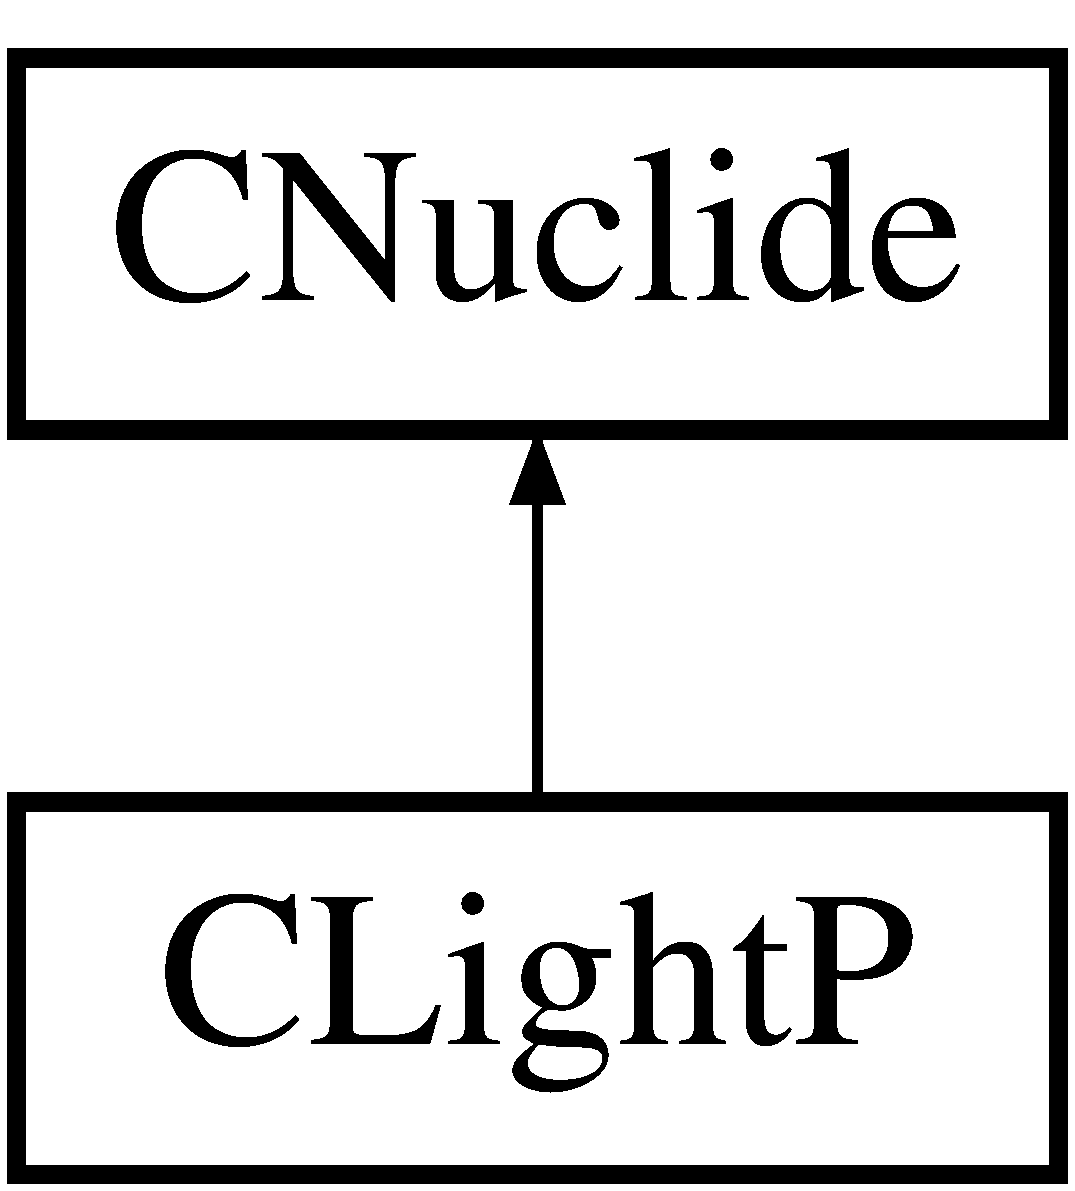
\includegraphics[height=2cm]{classCLightP}
\end{center}
\end{figure}
\subsection*{Public Member Functions}
\begin{CompactItemize}
\item 
\bf{CLight\-P} (int \bf{i\-Z}, int \bf{i\-A}, float f\-S, string s\-Name)
\begin{CompactList}\small\item\em constructor which creates a \doxyref{CTl\-Bar\-Dist}{p.}{classCTlBarDist} object \item\end{CompactList}\item 
\bf{CLight\-P} (int, int, float, \bf{CTl\-Bar\-Dist} $\ast$, \bf{CSig\-Bar\-Dist} $\ast$)
\begin{CompactList}\small\item\em constructor which uses an existing \doxyref{CTl\-Bar\-Dist}{p.}{classCTlBarDist} object \item\end{CompactList}\item 
\bf{$\sim$CLight\-P} ()
\begin{CompactList}\small\item\em destructor \item\end{CompactList}\end{CompactItemize}
\subsection*{Public Attributes}
\begin{CompactItemize}
\item 
\bf{CTl\-Bar\-Dist} $\ast$ \bf{tl\-Array}\label{classCLightP_beeff57d9152d9d9d8fb698467cf4206}

\begin{CompactList}\small\item\em gives transmission coefficients \item\end{CompactList}\item 
\bf{CSig\-Bar\-Dist} $\ast$ \bf{sig\-Bar\-Dist}\label{classCLightP_167d46c4fa628d3ade499f23a159ab60}

\begin{CompactList}\small\item\em gives inverse xsections for charged part \item\end{CompactList}\item 
float \bf{suppress}\label{classCLightP_3a274ab06295deecc7ac6bd92057f754}

\begin{CompactList}\small\item\em suppression factor to scale Hauser-Feshbach width \item\end{CompactList}\item 
float \bf{f\-MInertia}\label{classCLightP_445e25b6dc7b76252bb89a2af68512c3}

\begin{CompactList}\small\item\em moment of inertia of residue \item\end{CompactList}\item 
float \bf{f\-MInertia\-Orbit}\label{classCLightP_86367a01c26cb399668cb6d25162374a}

\begin{CompactList}\small\item\em moment of inerria for orbit of light P \item\end{CompactList}\item 
float \bf{separation\-Energy}\label{classCLightP_2ddf1727b00b3687c10127b8ae8ffcaf}

\begin{CompactList}\small\item\em separation energy in Me\-V \item\end{CompactList}\item 
float \bf{f\-Pair}\label{classCLightP_f964da045869c05bc4913f913271b7ac}

\begin{CompactList}\small\item\em pairing energy of residue \item\end{CompactList}\item 
float \bf{f\-Shell}\label{classCLightP_3028ded896484c0e66c30ef856128b7f}

\begin{CompactList}\small\item\em shell correction for residue \item\end{CompactList}\item 
\bf{CNuclide} \bf{residue}\label{classCLightP_c36a119fe62158837f065cadc78f3e32}

\begin{CompactList}\small\item\em contains info on the daughter nucleus \item\end{CompactList}\item 
bool \bf{odd}\label{classCLightP_2517c46d90ef1e23b9ab066df10b89e5}

\begin{CompactList}\small\item\em true for odd mass \item\end{CompactList}\item 
SStore\-Evap\-Vector \bf{store\-Evap}\label{classCLightP_e65852f55d5e4aba981a4bce6e052356}

\begin{CompactList}\small\item\em store evaporation info \item\end{CompactList}\item 
float \bf{width}\label{classCLightP_7c74b8d96d95e22d6db3e9d64b2b827e}

\begin{CompactList}\small\item\em decay width in Me\-V \item\end{CompactList}\item 
float \bf{r\-Light}\label{classCLightP_b3b9c314727310211e9337f4a3dbaf4f}

\begin{CompactList}\small\item\em radius of light particle in fm \item\end{CompactList}\end{CompactItemize}
\subsection*{Protected Attributes}
\begin{CompactItemize}
\item 
bool \bf{must\-Delete}\label{classCLightP_ac6f7bfdf2ad97ecb568d6e9cd1e50a4}

\begin{CompactList}\small\item\em bool to remember that we must delete the t\-LArray \item\end{CompactList}\end{CompactItemize}


\subsection{Detailed Description}
deals with a particular evaporation channel 

!

Class \doxyref{CLight\-P}{p.}{classCLightP} contains all the important information concerning a light particle evaporation channel, it has pointers to a c\-Tl\-Array class to calculate transmission coeff. 



\subsection{Constructor \& Destructor Documentation}
\index{CLightP@{CLight\-P}!CLightP@{CLightP}}
\index{CLightP@{CLightP}!CLightP@{CLight\-P}}
\subsubsection{\setlength{\rightskip}{0pt plus 5cm}CLight\-P::CLight\-P (int {\em i\-Z0}, int {\em i\-A0}, float {\em f\-J0}, string {\em name0})}\label{classCLightP_daea3b7b17cf535b2e068dc91d85e2e2}


constructor which creates a \doxyref{CTl\-Bar\-Dist}{p.}{classCTlBarDist} object 

\begin{Desc}
\item[Parameters:]
\begin{description}
\item[{\em i\-Z0}]proton number of particle \item[{\em i\-A0}]mass number of particle \item[{\em f\-J0}]spin of particle \item[{\em name0}]name of $\ast$.tl file containing transmission coefs. \end{description}
\end{Desc}
\index{CLightP@{CLight\-P}!CLightP@{CLightP}}
\index{CLightP@{CLightP}!CLightP@{CLight\-P}}
\subsubsection{\setlength{\rightskip}{0pt plus 5cm}CLight\-P::CLight\-P (int {\em i\-Z0}, int {\em i\-A0}, float {\em f\-J0}, \bf{CTl\-Bar\-Dist} $\ast$ {\em tl\-Array0}, \bf{CSig\-Bar\-Dist} $\ast$ {\em sig\-Bar\-Dist0})}\label{classCLightP_a313a4ee8253893578eb08770e229d45}


constructor which uses an existing \doxyref{CTl\-Bar\-Dist}{p.}{classCTlBarDist} object 

Alternative constructor which uses a previously defined transmission coeff object \doxyref{CTl\-Array}{p.}{classCTlArray} \begin{Desc}
\item[Parameters:]
\begin{description}
\item[{\em i\-Z0}]proton number of particle \item[{\em i\-A0}]mass number of particle \item[{\em f\-J0}]spin of particle \item[{\em tl\-Array0}]is the pointer to the object for transmission coefficients \item[{\em sig\-Bar\-Dist0}]is the pointer to the object for inverse xsections \end{description}
\end{Desc}
\index{CLightP@{CLight\-P}!~CLightP@{$\sim$CLightP}}
\index{~CLightP@{$\sim$CLightP}!CLightP@{CLight\-P}}
\subsubsection{\setlength{\rightskip}{0pt plus 5cm}CLight\-P::$\sim$CLight\-P ()}\label{classCLightP_17c53af5ce821817657330ce4bf5276e}


destructor 

Destructor 

The documentation for this class was generated from the following files:\begin{CompactItemize}
\item 
CLight\-P.h\item 
Light\-P.cpp\end{CompactItemize}

\section{CMass Class Reference}
\label{classCMass}\index{CMass@{CMass}}
mass excesses, pairing energy, etc  


{\tt \#include $<$CMass.h$>$}

\subsection*{Public Member Functions}
\begin{CompactItemize}
\item 
\bf{$\sim$CMass} ()
\item 
float \bf{get\-Exp\-Mass} (int i\-Z, int i\-A)
\item 
float \bf{get\-Cal\-Mass} (int i\-Z, int i\-A)
\item 
float \bf{get\-Shell\-Correction} (int i\-Z, int i\-A)
\item 
float \bf{get\-Shell\-Correction2} (int i\-Z, int i\-A)
\item 
float \bf{get\-Finite\-Range\-Mass} (int i\-Z, int i\-A)
\item 
float \bf{get\-Finite\-Range\-Mass} (float f\-Z, float f\-A)
\item 
float \bf{get\-Liquid\-Drop\-Mass} (int i\-Z, int i\-A)
\item 
float \bf{get\-Pairing} (int i\-Z, int i\-A)
\item 
float \bf{get\-Pairing2} (int i\-Z, int i\-A)
\end{CompactItemize}
\subsection*{Static Public Member Functions}
\begin{CompactItemize}
\item 
static \bf{CMass} $\ast$ \bf{instance} ()\label{classCMass_51bdc5af6783bf9c96a9aeab104caa94}

\begin{CompactList}\small\item\em instance member to make this a singleton \item\end{CompactList}\end{CompactItemize}
\subsection*{Public Attributes}
\begin{CompactItemize}
\item 
\bf{CChart} $\ast$ \bf{chart}\label{classCMass_123e5bd2e0b1741449817e01c45c377b}

\begin{CompactList}\small\item\em contains the considered region of the chart of nuclides \item\end{CompactList}\end{CompactItemize}
\subsection*{Protected Member Functions}
\begin{CompactItemize}
\item 
\bf{CMass} ()
\begin{CompactList}\small\item\em constructor \item\end{CompactList}\item 
void \bf{Read\-FRDMFile} ()
\item 
void \bf{Read\-Thomas\-Fermi\-File} ()
\end{CompactItemize}
\subsection*{Protected Attributes}
\begin{CompactItemize}
\item 
float $\ast$ \bf{f\-Exp\-Mass}\label{classCMass_94b681f2a0949f6e3abbcb1872e3569a}

\begin{CompactList}\small\item\em experimental mass array \item\end{CompactList}\item 
float $\ast$ \bf{f\-Cal\-Mass}\label{classCMass_d1d4e9cfdd75aa6a361ab4131a9e3250}

\begin{CompactList}\small\item\em experimental mass array \item\end{CompactList}\item 
float $\ast$ \bf{f\-FRM}\label{classCMass_b664f2eba3bb5973a5f3a41c5a929f94}

\begin{CompactList}\small\item\em finite range mass array \item\end{CompactList}\item 
float $\ast$ \bf{f\-Pair}\label{classCMass_74d98a8a5a4a1cbdc1532aaf5408c026}

\begin{CompactList}\small\item\em pairing correction \item\end{CompactList}\item 
float $\ast$ \bf{f\-Shell}\label{classCMass_b22cbf6a40128e4aa1460b9469e1ab8b}

\begin{CompactList}\small\item\em shell correction \item\end{CompactList}\item 
float $\ast$ \bf{f\-Shell2}\label{classCMass_32b6d3dcb143489ed987450bd243fd83}

\begin{CompactList}\small\item\em shell correction \item\end{CompactList}\end{CompactItemize}
\subsection*{Static Protected Attributes}
\begin{CompactItemize}
\item 
static \bf{CMass} $\ast$ \bf{f\-Instance} = 0\label{classCMass_a92566988e892bcfc9a17bb20e55f32c}

\begin{CompactList}\small\item\em instance member to make tis a singleton \item\end{CompactList}\end{CompactItemize}


\subsection{Detailed Description}
mass excesses, pairing energy, etc 

!

Class associated with returning quanties associated with the mass formula 



\subsection{Constructor \& Destructor Documentation}
\index{CMass@{CMass}!CMass@{CMass}}
\index{CMass@{CMass}!CMass@{CMass}}
\subsubsection{\setlength{\rightskip}{0pt plus 5cm}CMass::CMass ()\hspace{0.3cm}{\tt  [protected]}}\label{classCMass_2961afaaf4f193c19108d67a589072f3}


constructor 

Constructor \index{CMass@{CMass}!~CMass@{$\sim$CMass}}
\index{~CMass@{$\sim$CMass}!CMass@{CMass}}
\subsubsection{\setlength{\rightskip}{0pt plus 5cm}CMass::$\sim$CMass ()}\label{classCMass_ea23d00a8bcab0fd04aae37739509df0}


Destructor 

\subsection{Member Function Documentation}
\index{CMass@{CMass}!getCalMass@{getCalMass}}
\index{getCalMass@{getCalMass}!CMass@{CMass}}
\subsubsection{\setlength{\rightskip}{0pt plus 5cm}float CMass::get\-Cal\-Mass (int {\em i\-Z}, int {\em i\-A})}\label{classCMass_fd7aa662a139853822a373e3098bf3fa}


Returns the calculated mass excess from Moller and Nix

\begin{Desc}
\item[Parameters:]
\begin{description}
\item[{\em i\-Z}]is the proton number \item[{\em i\-A}]is the mass number \end{description}
\end{Desc}
\index{CMass@{CMass}!getExpMass@{getExpMass}}
\index{getExpMass@{getExpMass}!CMass@{CMass}}
\subsubsection{\setlength{\rightskip}{0pt plus 5cm}float CMass::get\-Exp\-Mass (int {\em i\-Z}, int {\em i\-A})}\label{classCMass_2431d9c00dc5a3835e14af2c6d61a764}


Returns the experimental mass excess

If teh experimental excess is not known, then the Moller Nix value is returned \begin{Desc}
\item[Parameters:]
\begin{description}
\item[{\em i\-Z}]is the proton number \item[{\em i\-A}]is the mass number \end{description}
\end{Desc}
\index{CMass@{CMass}!getFiniteRangeMass@{getFiniteRangeMass}}
\index{getFiniteRangeMass@{getFiniteRangeMass}!CMass@{CMass}}
\subsubsection{\setlength{\rightskip}{0pt plus 5cm}float CMass::get\-Finite\-Range\-Mass (float {\em f\-Z}, float {\em f\-A})}\label{classCMass_ded19b5cce25e6c94596b4e47dad6c84}


Calculates macroscopic finite range model masses of spherical nucleus using formula of Krappe, Nix, and Sierk.

Reference- (Phys Rev C20, 992 (1979)) modified to use the parameters of Moller + Nix Nucl. Phys. A361(1981) 117. Pairing correction term for odd-odd nuclei is included, as this is the most appropriate ground state for hot nuclei where shell and pairing effects have washed out. \begin{Desc}
\item[Parameters:]
\begin{description}
\item[{\em f\-Z}]is the proton number \item[{\em f\-A}]is the mass number \end{description}
\end{Desc}
\index{CMass@{CMass}!getFiniteRangeMass@{getFiniteRangeMass}}
\index{getFiniteRangeMass@{getFiniteRangeMass}!CMass@{CMass}}
\subsubsection{\setlength{\rightskip}{0pt plus 5cm}float CMass::get\-Finite\-Range\-Mass (int {\em i\-Z}, int {\em i\-A})}\label{classCMass_e0a6619be4dd82e97a7ba156af853c9e}


Calculates macroscopic finite range model masses of spherical nucleus using formula of Krappe, Nix, and Sierk.

Reference- (Phys Rev C20, 992 (1979)) modified to use the parameters of Moller + Nix Nucl. Phys. A361(1981) 117. Pairing correction term for odd-odd nuclei is included, as this is the most appropriate ground state for hot nuclei where shell and pairing effects have washed out. \begin{Desc}
\item[Parameters:]
\begin{description}
\item[{\em i\-Z}]is the proton number \item[{\em i\-A}]is the mass number \end{description}
\end{Desc}
\index{CMass@{CMass}!getLiquidDropMass@{getLiquidDropMass}}
\index{getLiquidDropMass@{getLiquidDropMass}!CMass@{CMass}}
\subsubsection{\setlength{\rightskip}{0pt plus 5cm}float CMass::get\-Liquid\-Drop\-Mass (int {\em i\-Z}, int {\em i\-A})}\label{classCMass_360701840914ad23d7ed3c3874ce0fc1}


Returns the liquid drop mass from moller and Nix \begin{Desc}
\item[Parameters:]
\begin{description}
\item[{\em i\-Z}]is the protom number \item[{\em i\-A}]is the mass number \end{description}
\end{Desc}
\index{CMass@{CMass}!getPairing@{getPairing}}
\index{getPairing@{getPairing}!CMass@{CMass}}
\subsubsection{\setlength{\rightskip}{0pt plus 5cm}float CMass::get\-Pairing (int {\em i\-Z}, int {\em i\-A})}\label{classCMass_57d4167da3dd5783572dffacd3f1f644}


Returns the pairing correction to the mass formula. From from Moller Nix is used. \begin{Desc}
\item[Parameters:]
\begin{description}
\item[{\em i\-Z}]is the proton number \item[{\em i\-A}]is the mass number \end{description}
\end{Desc}
\index{CMass@{CMass}!getPairing2@{getPairing2}}
\index{getPairing2@{getPairing2}!CMass@{CMass}}
\subsubsection{\setlength{\rightskip}{0pt plus 5cm}float CMass::get\-Pairing2 (int {\em i\-Z}, int {\em i\-A})}\label{classCMass_b8836a53fe6c21535f969d1c647317d4}


Returns the pairing correction to the mass formula. From from Moller Nix is used. \begin{Desc}
\item[Parameters:]
\begin{description}
\item[{\em i\-Z}]is the proton number \item[{\em i\-A}]is the mass number \end{description}
\end{Desc}
\index{CMass@{CMass}!getShellCorrection@{getShellCorrection}}
\index{getShellCorrection@{getShellCorrection}!CMass@{CMass}}
\subsubsection{\setlength{\rightskip}{0pt plus 5cm}float CMass::get\-Shell\-Correction (int {\em i\-Z}, int {\em i\-A})}\label{classCMass_4e81cde4776e71f637ff28cb7b04f20a}


Returns the shell correction from Moller and Nix

\begin{Desc}
\item[Parameters:]
\begin{description}
\item[{\em i\-Z}]is the proton number \item[{\em i\-A}]is the mass number \end{description}
\end{Desc}
\index{CMass@{CMass}!getShellCorrection2@{getShellCorrection2}}
\index{getShellCorrection2@{getShellCorrection2}!CMass@{CMass}}
\subsubsection{\setlength{\rightskip}{0pt plus 5cm}float CMass::get\-Shell\-Correction2 (int {\em i\-Z}, int {\em i\-A})}\label{classCMass_bb1cecf8c19cba4c047d8376f0ff4895}


Returns the shell correction from Moller and Nix

\begin{Desc}
\item[Parameters:]
\begin{description}
\item[{\em i\-Z}]is the proton number \item[{\em i\-A}]is the mass number \end{description}
\end{Desc}
\index{CMass@{CMass}!ReadFRDMFile@{ReadFRDMFile}}
\index{ReadFRDMFile@{ReadFRDMFile}!CMass@{CMass}}
\subsubsection{\setlength{\rightskip}{0pt plus 5cm}void CMass::Read\-FRDMFile ()\hspace{0.3cm}{\tt  [protected]}}\label{classCMass_95df5960907d3cde94a79ba1de582681}


Reads in the mass table from Moller and Nix \index{CMass@{CMass}!ReadThomasFermiFile@{ReadThomasFermiFile}}
\index{ReadThomasFermiFile@{ReadThomasFermiFile}!CMass@{CMass}}
\subsubsection{\setlength{\rightskip}{0pt plus 5cm}void CMass::Read\-Thomas\-Fermi\-File ()\hspace{0.3cm}{\tt  [protected]}}\label{classCMass_f1fa180e06c50061df38460b1116de82}


Reads in the mass table from the Thomas Fermi Model of Myers and Swietcki 

The documentation for this class was generated from the following files:\begin{CompactItemize}
\item 
CMass.h\item 
Mass.cpp\end{CompactItemize}

\section{CNucleus Class Reference}
\label{classCNucleus}\index{CNucleus@{CNucleus}}
Hauser-Feshbach, Bohr-Wheeler, Morretto, formulisms.  


{\tt \#include $<$CNucleus.h$>$}

Inheritance diagram for CNucleus::\begin{figure}[H]
\begin{center}
\leavevmode
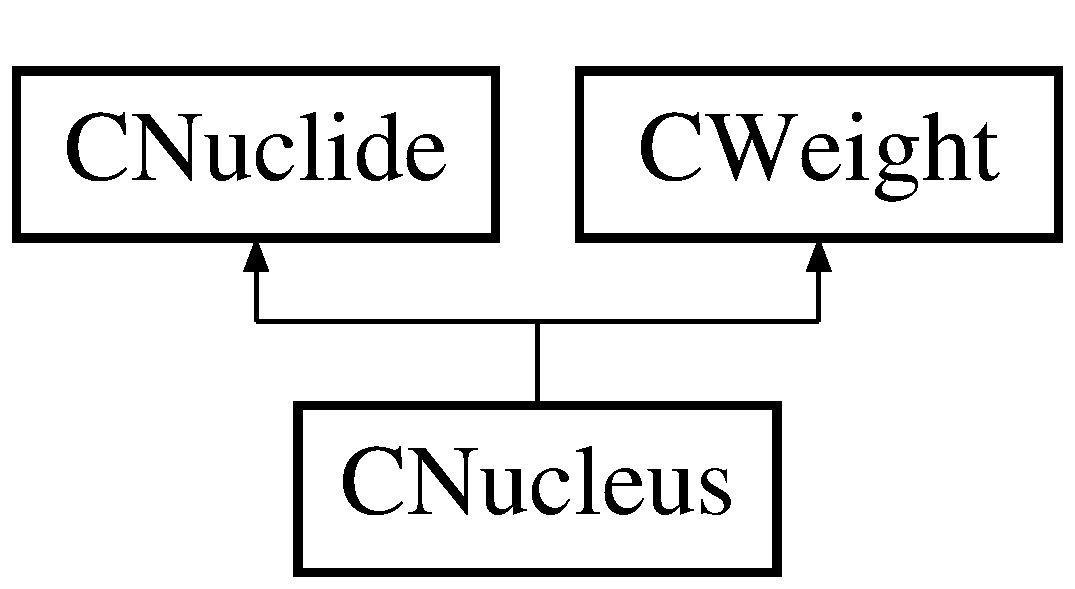
\includegraphics[height=2cm]{classCNucleus}
\end{center}
\end{figure}
\subsection*{Public Member Functions}
\begin{CompactItemize}
\item 
float \bf{evaporation\-Width} ()
\item 
float \bf{Bohr\-Wheeler\-Width} ()
\item 
float \bf{Lestone\-Fission\-Width} ()
\item 
float \bf{Lestone\-Correction} (float Usaddle, float mom\-Inertia\-Eff, short i\-Af\-An)
\item 
\bf{CNucleus} (int \bf{i\-Z}, int \bf{i\-A})
\item 
\bf{CNucleus} (int \bf{i\-Z}, int \bf{i\-A}, float \bf{f\-Ex}, float \bf{f\-J})
\item 
\bf{$\sim$CNucleus} ()
\item 
float \bf{get\-Sum\-Gamma\-Energy} ()
\item 
int \bf{getn\-Gamma\-Rays} ()
\item 
float \bf{get\-Gamma\-Ray\-Energy} (int number)
\item 
float \bf{get\-Time} ()
\item 
void \bf{set\-New\-Isotope} (int i\-Z0, int i\-A0, float f\-Ex0, float f\-J0)
\item 
void \bf{set\-Compound\-Nucleus} (float f\-Ex0, float f\-J0)
\item 
void \bf{set\-Compound\-Nucleus} (float f\-Ex0, double d\-J0)
\item 
void \bf{set\-Compound\-Nucleus} (double d\-Ex0, float f\-J0)
\item 
void \bf{set\-Compound\-Nucleus} (double d\-Ex0, double d\-J0)
\item 
void \bf{set\-Spin\-Axis} (\bf{CAngle} angle)
\item 
void \bf{set\-Spin\-Axis\-Degrees} (\bf{CAngle} angle)
\item 
void \bf{set\-Velocity\-Polar} (float=0., float=0., float=0.)
\item 
void \bf{set\-Velocity\-Cartesian} (float vx=0., float vy=0., float vz=0.)
\item 
void \bf{reset} ()
\item 
void \bf{print} ()
\item 
void \bf{print\-Stable\-Products} ()
\item 
void \bf{print\-All\-Products} ()
\item 
void \bf{v\-CMof\-All\-Products} ()
\item 
void \bf{energy\-Conservation} ()
\item 
\bf{CNucleus} $\ast$ \bf{get\-Products} (int=-1)
\item 
\bf{CNucleus} $\ast$ \bf{get\-Parent} ()
\item 
\bf{CNucleus} $\ast$ \bf{get\-Light\-Daughter} ()
\item 
\bf{CNucleus} $\ast$ \bf{get\-Heavy\-Daughter} ()
\item 
\bf{CNucleus} $\ast$ \bf{get\-Compound\-Nucleus} ()
\item 
int \bf{get\-Number\-Of\-Products} ()
\item 
int \bf{get\-Zmax\-Evap} ()
\item 
void \bf{excite} (float, float)
\item 
void \bf{excite} (float, double)
\item 
void \bf{excite} (double, float)
\item 
void \bf{excite} (double, double)
\item 
void \bf{excite} (float)
\item 
float \bf{get\-Theta} ()
\item 
float \bf{get\-Theta\-Degrees} ()
\item 
\bf{CAngle} \bf{get\-Angle} ()
\item 
\bf{CAngle} \bf{get\-Angle\-Degrees} ()
\item 
float \bf{get\-KE} ()
\item 
float \bf{get\-Velocity} ()
\item 
float \bf{get\-Momentum} ()
\item 
float $\ast$ \bf{get\-Velocity\-Vector} ()
\item 
float $\ast$ \bf{get\-Momentum\-Vector} ()
\item 
void \bf{decay} ()
\item 
bool \bf{is\-Asymmetric\-Fission} ()
\item 
bool \bf{is\-Symmetric\-Fission} ()
\item 
bool \bf{is\-Not\-Statistical} ()
\item 
bool \bf{is\-Saddle\-To\-Scission} ()
\item 
bool \bf{is\-Residue} ()
\item 
int \bf{get\-Mult\-Post} ()
\item 
int \bf{get\-Mult\-Pre} ()
\item 
int \bf{get\-Mult\-Post\-Light} ()
\item 
int \bf{get\-Mult\-Post\-Heavy} ()
\item 
int \bf{get\-Mult\-Pre\-Saddle} ()
\item 
int \bf{get\-Mult\-Saddle\-To\-Scission} ()
\item 
float \bf{get\-Fission\-Time\-Symmetric} (float \&\bf{time\-Scission})
\item 
float \bf{get\-Fission\-Time\-Asymmetric} ()
\item 
float \bf{get\-Decay\-Width} ()
\item 
float \bf{get\-Log\-Level\-Density} ()
\item 
void \bf{print\-Parameters} ()
\end{CompactItemize}
\subsection*{Static Public Member Functions}
\begin{CompactItemize}
\item 
static void \bf{reset\-Global} ()
\item 
static void \bf{set\-Time\-Transient} (float time)
\item 
static void \bf{set\-Fission\-Scale\-Factor} (float factor)
\item 
static void \bf{set\-Bar\-Width} (float width)
\item 
static void \bf{set\-Delta\-E} (float de0)
\item 
static void \bf{set\-Threshold} (float threshold0)
\item 
static void \bf{set\-Add\-To\-Fis\-Barrier} (float bar\-Add0)
\item 
static void \bf{set\-No\-IMF} ()
\item 
static void \bf{set\-Yes\-IMF} ()
\item 
static void \bf{set\-Lestone} ()
\item 
static void \bf{set\-Bohr\-Wheeler} ()
\item 
static void \bf{set\-Solution} (int isol)
\item 
static void \bf{set\-Evap\-Mode} (int i\-HF0=2)
\item 
static void \bf{set\-User\-GDR} (bool mode=true)
\item 
static float \bf{get\-Time\-Transient} ()
\item 
static float \bf{get\-Fission\-Scale\-Factor} ()
\item 
static float \bf{get\-Bar\-Width} ()
\item 
static float \bf{get\-Delta\-E} ()
\item 
static float \bf{get\-Threshold} ()
\item 
static float \bf{get\-Add\-To\-Fis\-Barrier} ()
\end{CompactItemize}
\subsection*{Public Attributes}
\begin{CompactItemize}
\item 
bool \bf{abort\-Event}\label{classCNucleus_e7093b3a71b1ef30c899afe2bff3a75a}

\begin{CompactList}\small\item\em abort the event \item\end{CompactList}\item 
int \bf{origin}\label{classCNucleus_f4e2c66d862fe72f2152a3fea8f14590}

\begin{CompactList}\small\item\em specifies the origin of the fragment, prefission, post , etc \item\end{CompactList}\item 
int \bf{origin2}\label{classCNucleus_aa0d1c7aba08b8669c5b3a15ca393e95}

\begin{CompactList}\small\item\em specifies the origin of the fragment, prefission, post , etc \item\end{CompactList}\end{CompactItemize}
\subsection*{Static Public Attributes}
\begin{CompactItemize}
\item 
static float const \bf{pi} = acos(-1.)\label{classCNucleus_8b2e3247e90428054c7018ce3a9795dd}

\begin{CompactList}\small\item\em 3.14159 \item\end{CompactList}\item 
static double const \textbf{Ek\-Fraction} = 0.01\label{classCNucleus_3a2a8a6e1f86db6b1d5ecb180a296713}

\end{CompactItemize}
\subsection*{Protected Member Functions}
\begin{CompactItemize}
\item 
void \bf{saddle\-To\-Scission} ()
\item 
void \bf{mass\-Asymmetry} (bool)
\item 
float \bf{select\-J} (float, float, float, float)
\item 
float \bf{S2Loop} (float Ekvalue)
\item 
float \bf{S2Width} (float Ekvalue)
\item 
float \bf{Ek\-Width} (float ek)
\item 
void \bf{get\-Spin} (bool saddle)
\item 
float \bf{Ek\-Loop} ()
\item 
float \bf{get\-Sum\-Tl} (float, float)
\item 
float \bf{get\-Width\-ZA} (float, short)
\item 
void \bf{angle\-Evap} ()
\item 
void \bf{angle\-Isotropic} ()
\item 
void \bf{angle\-Gamma} ()
\item 
void \bf{binary\-Decay} ()
\item 
void \bf{excite\-Scission} (float, float, bool sym=1)
\item 
float \bf{asy\-Fission\-Width} ()
\item 
float \bf{asy\-Fission\-Width\-ZA} ()
\item 
float \bf{asy\-Fission\-Width\-BW} ()
\item 
void \bf{force8Be} ()
\item 
void \bf{force5Li} ()
\item 
void \bf{force5He} ()
\item 
void \bf{force9B} ()
\item 
float \bf{evaporation\-Width\-SS} ()
\item 
float \bf{gamma\-Width} ()
\item 
float \bf{gamma\-Width\-E1GDR} ()
\item 
float \bf{gamma\-Width\-Multipole} (int)
\item 
float \bf{hauser\-Feshbach} (int)
\item 
float \bf{weiskopf} (bool saddle)
\item 
void \bf{asy\-Fission\-Divide} ()
\item 
void \bf{recursive\-Decay} ()
\item 
void \bf{split} (\bf{CAngle})
\end{CompactItemize}
\subsection*{Protected Attributes}
\begin{CompactItemize}
\item 
float \bf{Ecoul}\label{classCNucleus_9f51c4abb70f1adbedce26c870a09e40}

\begin{CompactList}\small\item\em Coulomb barrier (Hauser\-Feshbach). \item\end{CompactList}\item 
bool \bf{not\-Statistical}\label{classCNucleus_8674956cb95a57c427bf686dcaa36d15}

\begin{CompactList}\small\item\em this does not decay statistically, evap. frag. only \item\end{CompactList}\item 
short unsigned \bf{not\-Statistical\-Mode}\label{classCNucleus_a8a6f095fac5317ace58834b19694dd7}

\begin{CompactList}\small\item\em specifies type of non\-Statisical decay \item\end{CompactList}\item 
float \bf{f\-Pairing}\label{classCNucleus_75e46b261560250eaf707dc70f0ef5c2}

\begin{CompactList}\small\item\em pairing energy \item\end{CompactList}\item 
float \bf{f\-Shell}\label{classCNucleus_63be1f3c94200c33987e505c116e48e4}

\begin{CompactList}\small\item\em shell correction \item\end{CompactList}\item 
float \bf{f\-U0}\label{classCNucleus_ffdd5bc8fddd877c402c362fe0e5f328}

\begin{CompactList}\small\item\em thermal excitation energy \item\end{CompactList}\item 
float \bf{Erot}\label{classCNucleus_07c59d444213ba5e49e4fe0cf0b2f6ac}

\begin{CompactList}\small\item\em yrast energy \item\end{CompactList}\item 
float \bf{Jmax}\label{classCNucleus_3b38fc85190408ba31be4f937869d82a}

\begin{CompactList}\small\item\em max spin with a fission barrier \item\end{CompactList}\item 
float \bf{f\-MInertia}\label{classCNucleus_754b0d967e466828e054760118003439}

\begin{CompactList}\small\item\em spherical moment of inertia \item\end{CompactList}\item 
float \bf{log\-Level\-Density}\label{classCNucleus_93434cd2f1835487f3fd5838a0329516}

\begin{CompactList}\small\item\em store the log of the level density of the nucleus \item\end{CompactList}\item 
float \bf{temp}\label{classCNucleus_1a4d6de0550a45c3568b51ec8b764a87}

\begin{CompactList}\small\item\em nuclear temperature \item\end{CompactList}\item 
int \bf{fission\-Z}\label{classCNucleus_07e770cb35ede22fe8755ffaba172e72}

\begin{CompactList}\small\item\em proton number of fission fragment \item\end{CompactList}\item 
int \bf{fission\-A}\label{classCNucleus_d213539018fa3628166e37393041afc0}

\begin{CompactList}\small\item\em mass number of fission fragment \item\end{CompactList}\item 
int \bf{fissioning\-Z}\label{classCNucleus_cd82c11c9bfa2da866ea4c3c4aaba6b4}

\begin{CompactList}\small\item\em proton number of fission parent \item\end{CompactList}\item 
int \bf{fissioning\-A}\label{classCNucleus_d41680104321b05aa44ca206d0041e8e}

\begin{CompactList}\small\item\em mass number of fission parent \item\end{CompactList}\item 
int \bf{i\-Z1\_\-IMF\_\-Max}\label{classCNucleus_ac06d46691f3d89495ab0588246f807f}

\begin{CompactList}\small\item\em maximum Z for IMF emission \item\end{CompactList}\item 
float \bf{fission\-U}\label{classCNucleus_59978fb0577ff47f85e0ff70d5bff738}

\begin{CompactList}\small\item\em thermal excitation energy of both fission fragments \item\end{CompactList}\item 
float \bf{Edef\-Scission}\label{classCNucleus_66928e8717b00eee3528d0a41fbe6f1c}

\begin{CompactList}\small\item\em deformation energy of the scission configuration \item\end{CompactList}\item 
bool \bf{saddle\-To\-Sciss}\label{classCNucleus_b19cf9a8f277af3cdeb4041e2d34e5b1}

\begin{CompactList}\small\item\em indicated decay during saddle-to-scission transition \item\end{CompactList}\item 
float \bf{time\-Since\-Saddle}\label{classCNucleus_32e4c5b3c8eac249f0ff08f5e3b48278}

\begin{CompactList}\small\item\em stores the time since the saddle was crossed \item\end{CompactList}\item 
float \bf{time\-Since\-Start}\label{classCNucleus_f7b0df1b93f3d98bb611317d96b0aa84}

\begin{CompactList}\small\item\em stores the time since the decay began \item\end{CompactList}\item 
bool \bf{need\-Symmetric\-Fission}\label{classCNucleus_0ad7f9cdf22bd0b01d02ce590ad79572}

\begin{CompactList}\small\item\em indicated the Bohr-Wheeler width is needed \item\end{CompactList}\item 
float \bf{time\-Scission}\label{classCNucleus_c1c5cc107cc70bf7799e092aa59181a9}

\begin{CompactList}\small\item\em time required to go from saddle to scission \item\end{CompactList}\item 
int \bf{HF}\label{classCNucleus_01a6ee7880fed411d75adc4af7fa88df}

\begin{CompactList}\small\item\em evaporation mode chosen for a given decay \item\end{CompactList}\item 
\bf{CScission} \bf{scission}\label{classCNucleus_695aaf5a4264266303601a24b3f19963}

\begin{CompactList}\small\item\em gives scission energeis, etc \item\end{CompactList}\item 
bool \bf{b\-Stable}\label{classCNucleus_04b42c19af6888180ffb77ca7cbdf141}

\begin{CompactList}\small\item\em indicated this nucleus is particle-stable \item\end{CompactList}\item 
\bf{CAngle} \bf{spin}\label{classCNucleus_7719a0eacc9f415cec5040059218b88d}

\begin{CompactList}\small\item\em orientation of the spin axis \item\end{CompactList}\item 
float \bf{velocity} [3]\label{classCNucleus_aff04dba4f6e855c899601275918f9be}

\begin{CompactList}\small\item\em velocity vector of nucleus in cm/ns \item\end{CompactList}\item 
float \bf{momentum} [3]\label{classCNucleus_a37cd21aeaeb87c23a0620700163bbe7}

\begin{CompactList}\small\item\em momentum vector in Me\-V/c \item\end{CompactList}\item 
\bf{CLight\-P} $\ast$ \bf{light\-P}\label{classCNucleus_caba2810b8d165ad5817de76fc989516}

\begin{CompactList}\small\item\em points to the light-particle decay mode \item\end{CompactList}\item 
float \bf{S2Start}\label{classCNucleus_dc7e540e4d0d081195cd07451db0a03e}

\begin{CompactList}\small\item\em Hauser-Feshback spin of daughter. \item\end{CompactList}\item 
float \bf{UMin}\label{classCNucleus_151065323ac9430395f1b532712f8eba}

\begin{CompactList}\small\item\em min thermal excitation energy in Hauser-Feshbach \item\end{CompactList}\item 
float \bf{Ecost\-Min}\label{classCNucleus_eb1f0dc0fc743ff598283ce3c44ff828}

\begin{CompactList}\small\item\em the min of the energetic cost of emitting light particles \item\end{CompactList}\item 
int \bf{l\-Min}\label{classCNucleus_29855967b78940b4f2c3c35ddab444ee}

\begin{CompactList}\small\item\em minimum orbital AM for Hauser-Feshbach \item\end{CompactList}\item 
int \bf{l\-Max}\label{classCNucleus_f0245579c51de36a2d07e2d374f379df}

\begin{CompactList}\small\item\em maximum orbital AM for Hauser-Feshbach \item\end{CompactList}\item 
float \bf{l\-Plus\-SMax}\label{classCNucleus_d3362662d4f9ce707b6e195a3a4553da}

\begin{CompactList}\small\item\em max value of l+S of evaporated particle \item\end{CompactList}\item 
float \bf{l\-Plus\-SMin}\label{classCNucleus_77b2303bf0111a8307661139464c0dd1}

\begin{CompactList}\small\item\em min value of l+S of evaporated particle \item\end{CompactList}\item 
float \bf{r\-Residue}\label{classCNucleus_2abcfce53673c7ecf8aadd958d9b550e}

\begin{CompactList}\small\item\em radius of daughter \item\end{CompactList}\item 
float \bf{r\-Light\-P}\label{classCNucleus_26b7d7cd05121215cc2204e6b8e07c69}

\begin{CompactList}\small\item\em radius of evaporated particle \item\end{CompactList}\item 
float \bf{S2}\label{classCNucleus_d0695564a88628e2a2c676cb6690424c}

\begin{CompactList}\small\item\em spin of daughter \item\end{CompactList}\item 
float \bf{EYrast2}\label{classCNucleus_a55ddbb76d85375a1a852bc04b61c7dc}

\begin{CompactList}\small\item\em rotational energy of daughter \item\end{CompactList}\item 
\bf{SStore\-Evap} $\ast$ \bf{store\-Evap}\label{classCNucleus_10520ca775f56a46c92776c15bfc754a}

\begin{CompactList}\small\item\em information of evap sub channels \item\end{CompactList}\item 
\bf{SStore\-Sub} $\ast$ \bf{store\-Sub}\label{classCNucleus_12071dc08bd68af6ce7a12212b2dca58}

\begin{CompactList}\small\item\em store info on l distribution \item\end{CompactList}\item 
int \bf{i\-Store}\label{classCNucleus_2f4f38445fb5d30ef9e2cdfc6f5fc5b8}

\begin{CompactList}\small\item\em actual number of evap sub channels \item\end{CompactList}\item 
short unsigned \bf{Evap\-Z2}\label{classCNucleus_f2fc6d972d0280cbdc3c887996da4234}

\begin{CompactList}\small\item\em proton number of daughter after evap. \item\end{CompactList}\item 
short unsigned \bf{Evap\-A2}\label{classCNucleus_a407604f754f376c417d3eb51d14c733}

\begin{CompactList}\small\item\em mass number of daughter after evap. \item\end{CompactList}\item 
short unsigned \bf{Evap\-Z1}\label{classCNucleus_9ccd194e2aa9eff5b543051f64fb0657}

\begin{CompactList}\small\item\em proton number of evaporated particle \item\end{CompactList}\item 
short unsigned \bf{Evap\-A1}\label{classCNucleus_ed67dc0e2a1b2fd2efa82ab4fc96c8b3}

\begin{CompactList}\small\item\em mass number of evaporated particle \item\end{CompactList}\item 
short unsigned \bf{Evap\-L}\label{classCNucleus_907b9c2b63c262c9b754981781a9218f}

\begin{CompactList}\small\item\em orbital AM of evaporated particle \item\end{CompactList}\item 
short unsigned \bf{Evap\-Mode}\label{classCNucleus_50fc53bcb2d614e3ccb4eeaddbeb1843}

\begin{CompactList}\small\item\em ID number of evap channel. \item\end{CompactList}\item 
float \bf{Evap\-Ex1}\label{classCNucleus_2b8d84026794c264d9ecb02d4e9b49aa}

\begin{CompactList}\small\item\em excitation ennergy of evap. particle \item\end{CompactList}\item 
float \bf{Evap\-Ex2}\label{classCNucleus_85eacf531f04fb3dad16c16f02f93ceb}

\begin{CompactList}\small\item\em excitation energy of daughter after evap. \item\end{CompactList}\item 
float \bf{Evap\-S2}\label{classCNucleus_cc42cb5f0e00f84985fee77b89e1a6f4}

\begin{CompactList}\small\item\em spin of daughter after evap \item\end{CompactList}\item 
float \bf{Evap\-S1}\label{classCNucleus_5c108577f3f971fb159aaa64f2ce42dc}

\begin{CompactList}\small\item\em spin of evaporated particle \item\end{CompactList}\item 
float \bf{Evap\-Ek}\label{classCNucleus_5ea2a497fc174a082f3ff0b25dd179d4}

\begin{CompactList}\small\item\em kinetic energy of evaporated particle (Me\-V) \item\end{CompactList}\item 
float \bf{Evap\-LPlus\-S}\label{classCNucleus_3e063fecf098db206488e4df14657700}

\begin{CompactList}\small\item\em toatl spin plus orbital AM of evaporated particle \item\end{CompactList}\item 
float \bf{Gamma\-Ex}\label{classCNucleus_21756bd02b8bb6c25a0c988c56262008}

\begin{CompactList}\small\item\em excitation energy after gamma emission \item\end{CompactList}\item 
float \bf{Gamma\-J}\label{classCNucleus_78f8853e9df1981231869f20961d48a0}

\begin{CompactList}\small\item\em spin after gamma emission \item\end{CompactList}\item 
int \bf{Gamma\-L}\label{classCNucleus_6bc78a6013952ac73a35eb406a773301}

\begin{CompactList}\small\item\em gamma type E1=1, E2 = 2 \item\end{CompactList}\item 
\bf{CNucleus} $\ast$ \bf{daughter\-Light}\label{classCNucleus_98e90369fddde884de5be981f2fa70fd}

\begin{CompactList}\small\item\em pointer to the lighter of the decay products \item\end{CompactList}\item 
\bf{CNucleus} $\ast$ \bf{daughter\-Heavy}\label{classCNucleus_d6cea02b67a65066e0285ce366fded9b}

\begin{CompactList}\small\item\em pointer to the heavier of the decay products \item\end{CompactList}\item 
\bf{CNucleus} $\ast$ \bf{parent}\label{classCNucleus_cd2ccf477ffcae85ba6bb86efe5d4cae}

\begin{CompactList}\small\item\em pointer to the parent nucleus \item\end{CompactList}\item 
bool \bf{b\-Residue}\label{classCNucleus_6c9c08f0b5d1597a2480e4645a41cd70}

\begin{CompactList}\small\item\em true if decay produced an evaporation residue \item\end{CompactList}\item 
bool \bf{b\-Symmetric\-Fission}\label{classCNucleus_332fd860f164e7a4e671285e5a5db0d5}

\begin{CompactList}\small\item\em true if decay resulted in symmetric fission \item\end{CompactList}\item 
bool \bf{b\-Asymmetric\-Fission}\label{classCNucleus_9eff0ffee9653dbd75ff2b665e2ebd26}

\begin{CompactList}\small\item\em true if decay resulted in asymmetric fission \item\end{CompactList}\item 
int \bf{mult\-Post\-Light}\label{classCNucleus_516d49562c7f5d6af98a7dc5a293f5fe}

\begin{CompactList}\small\item\em number of post-fission neutrons for lighter ff \item\end{CompactList}\item 
int \bf{mult\-Post\-Heavy}\label{classCNucleus_ca92f7a4d81ab39e230c3c20d6b0b3a8}

\begin{CompactList}\small\item\em number of post-fission neutrons for heavier ff \item\end{CompactList}\item 
int \bf{mult\-Pre\-Saddle}\label{classCNucleus_e1d40b4b343bd28a243c6c44c5f5e3d3}

\begin{CompactList}\small\item\em number of pre-scission neutrons emitted \item\end{CompactList}\item 
int \bf{mult\-Saddle\-To\-Scission}\label{classCNucleus_561b70bf56addf062d1e95c0793a5568}

\begin{CompactList}\small\item\em number of neutrons emitted between saddle and scission \item\end{CompactList}\item 
float \bf{sigma2}\label{classCNucleus_144194ae9e50c871ddf8c71e8eef8056}

\begin{CompactList}\small\item\em variance of fission mass distribution \item\end{CompactList}\item 
float \bf{sym\-Saddle\-Point}\label{classCNucleus_e33ebad4f9ae1e3b63e09f786d6027f0}

\begin{CompactList}\small\item\em symmetric saddle point energy \item\end{CompactList}\end{CompactItemize}
\subsection*{Static Protected Attributes}
\begin{CompactItemize}
\item 
static bool const \bf{no\-Symmetry} = 1\label{classCNucleus_9c5059aee22050c40b24446df581452e}

\begin{CompactList}\small\item\em true - old gemini with Morreto for all \item\end{CompactList}\item 
static float const \bf{viscosity\_\-scission} = 1.\label{classCNucleus_3921a219f62d2bf70b46c056d40b7980}

\begin{CompactList}\small\item\em viscosity during saddle\-Tosciss \item\end{CompactList}\item 
static float const \bf{viscosity\_\-saddle} = 1.5\label{classCNucleus_efe54ace1a2ab1a3585bb66d0614366d}

\begin{CompactList}\small\item\em viscosity during saddle\-Tosciss \item\end{CompactList}\item 
static float \bf{time\-Transient} = 0.\label{classCNucleus_7f59872f6f7e9c12e3fb093cfa7869b8}

\begin{CompactList}\small\item\em transient fission delay \item\end{CompactList}\item 
static float \bf{fission\-Scale\-Factor} = 1.00\label{classCNucleus_b32cf3076985253499e437b1cf9bc428}

\begin{CompactList}\small\item\em fission width scaled by this factor \item\end{CompactList}\item 
static float \bf{bar\-Add} = 0.\label{classCNucleus_01e8c2c8984730b2f5d62f9b9f91276f}

\begin{CompactList}\small\item\em adds to Sierk fission barrier \item\end{CompactList}\item 
static unsigned \bf{i\-Point} = -1\label{classCNucleus_9b46475eccd2550c39ee46fdbe570d87}

\begin{CompactList}\small\item\em pointer to array of stable fragments \item\end{CompactList}\item 
static int \bf{i\-HF} = 2\label{classCNucleus_1801ecefacee18afca1f479cbdf1bf94}

\begin{CompactList}\small\item\em set evaporation mode \item\end{CompactList}\item 
static bool \bf{no\-IMF} = 0\label{classCNucleus_90c9828bc7d3d0710aabe21b42fa629f}

\begin{CompactList}\small\item\em no imf emission is considered \item\end{CompactList}\item 
static bool \bf{Bohr\-Wheeler} = 1\label{classCNucleus_eb534c43c64db81a83dd76540e5e18ec}

\begin{CompactList}\small\item\em no imf emission is considered \item\end{CompactList}\item 
static short unsigned \bf{Zshell} = 2\label{classCNucleus_8bad711d5d83154f008060fce7bb5cb4}

\begin{CompactList}\small\item\em enforce shell effects in evaporation \item\end{CompactList}\item 
static \bf{CYrast} $\ast$ \bf{yrast}\label{classCNucleus_56fe03f6c281ec44145212ee40f419e6}

\begin{CompactList}\small\item\em gives fission barriers and rotational energies \item\end{CompactList}\item 
static \bf{CLevel\-Density} $\ast$ \bf{level\-Density}\label{classCNucleus_be8c98a1bbd49777402e0ca1b1bce748}

\begin{CompactList}\small\item\em gives level densities \item\end{CompactList}\item 
static \bf{CGdr} $\ast$ \bf{GDR}\label{classCNucleus_cdbaca13cb7cf36fb7c8995dd18a23da}

\begin{CompactList}\small\item\em uder defined GDR line shape \item\end{CompactList}\item 
static float const \bf{r0} = 1.16\label{classCNucleus_dde840341ee9fc96b7f0ed9f1ace2d45}

\begin{CompactList}\small\item\em radius const (fm) \item\end{CompactList}\item 
static float const \bf{sep} = 2.\label{classCNucleus_59b57c0fca3af933564d4be6b3396370}

\begin{CompactList}\small\item\em separation between fragments \item\end{CompactList}\item 
static float \bf{threshold} = .001\label{classCNucleus_aeb319ff1406939cb22c0a58c1ccc6e7}

\begin{CompactList}\small\item\em used to turn off unlikey evaporations \item\end{CompactList}\item 
static \bf{CEvap} $\ast$ \bf{evap}\label{classCNucleus_9898e1af21af0a50f75d86098667c60e}

\begin{CompactList}\small\item\em stores info on evaporated particles \item\end{CompactList}\item 
static short unsigned const \bf{l\-Max\-Quantum} = 50\label{classCNucleus_461f1b5cdf7c0143db6d4bf55bffc7f4}

\begin{CompactList}\small\item\em number of l-waves to store angular dist \item\end{CompactList}\item 
static float \bf{de} = 1.0\label{classCNucleus_76b7be5a568abe8895fdf335cee683ff}

\begin{CompactList}\small\item\em kinetic-energy interval for integrating in Hauser-Feshb \item\end{CompactList}\item 
static \bf{CAngle\-Dist} \bf{angle\-Dist}\label{classCNucleus_cf4ddc841a216bfb7fd1e3a56b7b692d}

\begin{CompactList}\small\item\em selects angular distributions of decays \item\end{CompactList}\item 
static float const \bf{gamma\-Inhibition} [3] = \{0.,.025,9.\}\label{classCNucleus_78515e687b420a5799034204d3924a91}

\begin{CompactList}\small\item\em scaling of gamma width from Weisskopf value \item\end{CompactList}\item 
static float const \bf{wue} [3] = \{0.,6.8e-8,4.9e-14\}\label{classCNucleus_ab8ceb4fc9ef268e2354ff7d0ebd8af5}

\begin{CompactList}\small\item\em coeff for Weisskopf units (gamma decay) \item\end{CompactList}\item 
static int const \bf{Nproducts}\label{classCNucleus_c5d3dd0a2c063545e93c329e0eeac9aa}

\begin{CompactList}\small\item\em total number of possible decay products from all decays \item\end{CompactList}\item 
static vector$<$ \bf{CNucleus} $\ast$ $>$ \bf{all\-Products}\label{classCNucleus_376354d934311d2fa839b9fa5e49397a}

\begin{CompactList}\small\item\em array of pointer to all decay products (stable or intermediate) \item\end{CompactList}\item 
static vector$<$ \bf{CNucleus} $\ast$ $>$ \bf{stable\-Products}\label{classCNucleus_82ddb346a9f87b53d0dfb18551d7cace}

\begin{CompactList}\small\item\em array of pointers to all stable decay products for all CN decays \item\end{CompactList}\item 
static float const \bf{k\-Rotate} = 41.563\label{classCNucleus_4335fec8a155079842040f691b25b770}

\begin{CompactList}\small\item\em constant to calculated rotational energy \item\end{CompactList}\item 
static float \bf{sum\-Gamma\-Energy} = 0.\label{classCNucleus_0f81e0be4be19db07d1b819ba5902947}

\begin{CompactList}\small\item\em store the energy emitted in gamma rays \item\end{CompactList}\item 
static vector$<$ float $>$ \bf{Gamma\-Ray\-Energy}\label{classCNucleus_d02df9609ff19fca8a7dad80395da589}

\begin{CompactList}\small\item\em store each gamma ray energy \item\end{CompactList}\item 
static int \bf{n\-Gamma\-Rays} = 0\label{classCNucleus_f91eb2b5abf86b25a1a4db561f4e532e}

\begin{CompactList}\small\item\em number of emitted gamma rays \item\end{CompactList}\item 
static bool \bf{GDRParam} = false\label{classCNucleus_38ee9aa5f523827bb361ad24f3fe7c3e}

\begin{CompactList}\small\item\em if true, the standard formula for GDR decay width is used, if false the parametrized version \item\end{CompactList}\end{CompactItemize}


\subsection{Detailed Description}
Hauser-Feshbach, Bohr-Wheeler, Morretto, formulisms. 

!

Class \doxyref{CNucleus}{p.}{classCNucleus} impliments the GEMINI statistical mode code. It follows the decay of a compound nucleus by a sequential series of binary decays. The decay widths are calculated with Hauser-Feshbash formulism for light particles and Morreto's transition-state formulism for other binary decays 



\subsection{Constructor \& Destructor Documentation}
\index{CNucleus@{CNucleus}!CNucleus@{CNucleus}}
\index{CNucleus@{CNucleus}!CNucleus@{CNucleus}}
\subsubsection{\setlength{\rightskip}{0pt plus 5cm}CNucleus::CNucleus (int {\em i\-Z0}, int {\em i\-A0})}\label{classCNucleus_b884bdacef32d64c58c60f36aa358ccd}


constructor specifies the isotope. \begin{Desc}
\item[Parameters:]
\begin{description}
\item[{\em i\-Z0}]is the proton number \item[{\em i\-A0}]is the mass number \end{description}
\end{Desc}
\index{CNucleus@{CNucleus}!CNucleus@{CNucleus}}
\index{CNucleus@{CNucleus}!CNucleus@{CNucleus}}
\subsubsection{\setlength{\rightskip}{0pt plus 5cm}CNucleus::CNucleus (int {\em i\-Z0}, int {\em i\-A0}, float {\em f\-Ex0}, float {\em f\-J0})}\label{classCNucleus_a7a3dd1e0a497f33e5d835616d8a2d85}


Constructor specifying more parameters \begin{Desc}
\item[Parameters:]
\begin{description}
\item[{\em i\-Z0}]is proton number \item[{\em i\-A0}]is mass number \item[{\em f\-Ex0}]is excitation energy in Me\-V \item[{\em f\-J0}]is spin in hbar \end{description}
\end{Desc}
\index{CNucleus@{CNucleus}!~CNucleus@{$\sim$CNucleus}}
\index{~CNucleus@{$\sim$CNucleus}!CNucleus@{CNucleus}}
\subsubsection{\setlength{\rightskip}{0pt plus 5cm}CNucleus::$\sim$CNucleus ()}\label{classCNucleus_22e62673e10ef95522adef084f84880b}


destructor 

\subsection{Member Function Documentation}
\index{CNucleus@{CNucleus}!angleEvap@{angleEvap}}
\index{angleEvap@{angleEvap}!CNucleus@{CNucleus}}
\subsubsection{\setlength{\rightskip}{0pt plus 5cm}void CNucleus::angle\-Evap ()\hspace{0.3cm}{\tt  [protected]}}\label{classCNucleus_0f2ab2f51560245e50f5120f8ed8cc91}


Selects the angle and velocity of an evaporated product \index{CNucleus@{CNucleus}!angleGamma@{angleGamma}}
\index{angleGamma@{angleGamma}!CNucleus@{CNucleus}}
\subsubsection{\setlength{\rightskip}{0pt plus 5cm}void CNucleus::angle\-Gamma ()\hspace{0.3cm}{\tt  [protected]}}\label{classCNucleus_1e5bb153a21a26d85586bc816b3a5cfa}


Selects the angle and sin axis of a daughter product after gamma emission \index{CNucleus@{CNucleus}!angleIsotropic@{angleIsotropic}}
\index{angleIsotropic@{angleIsotropic}!CNucleus@{CNucleus}}
\subsubsection{\setlength{\rightskip}{0pt plus 5cm}void CNucleus::angle\-Isotropic ()\hspace{0.3cm}{\tt  [protected]}}\label{classCNucleus_aa53ef1ac682d391422bdbba0652d882}


selects the velocity of evaporated particles, the emission angles is assumed isotropic \index{CNucleus@{CNucleus}!asyFissionDivide@{asyFissionDivide}}
\index{asyFissionDivide@{asyFissionDivide}!CNucleus@{CNucleus}}
\subsubsection{\setlength{\rightskip}{0pt plus 5cm}void CNucleus::asy\-Fission\-Divide ()\hspace{0.3cm}{\tt  [protected]}}\label{classCNucleus_40be378f7da175ee00bf0db4c069ea2b}


Responsible for subdividing spin and excitation energy for asymmetry fission.

its uses a two-sphere approximation to get collective modes \index{CNucleus@{CNucleus}!asyFissionWidth@{asyFissionWidth}}
\index{asyFissionWidth@{asyFissionWidth}!CNucleus@{CNucleus}}
\subsubsection{\setlength{\rightskip}{0pt plus 5cm}float CNucleus::asy\-Fission\-Width ()\hspace{0.3cm}{\tt  [protected]}}\label{classCNucleus_49fa905c4ca5751be1c6b44c22a1f55c}


Calculates the asymmetric decay width in Me\-V from the gamma\-Z formalism.

if no\-Symmetry = 1 then it only includes channels outside of the fission peak \index{CNucleus@{CNucleus}!asyFissionWidthBW@{asyFissionWidthBW}}
\index{asyFissionWidthBW@{asyFissionWidthBW}!CNucleus@{CNucleus}}
\subsubsection{\setlength{\rightskip}{0pt plus 5cm}float CNucleus::asy\-Fission\-Width\-BW ()\hspace{0.3cm}{\tt  [protected]}}\label{classCNucleus_949c8af071a0e7707b30db291b9b5623}


Calculates the complex fragments decay widths in Me\-V where the total fission width all channels is normalised to the Bohr-Wheeler result. \index{CNucleus@{CNucleus}!asyFissionWidthZA@{asyFissionWidthZA}}
\index{asyFissionWidthZA@{asyFissionWidthZA}!CNucleus@{CNucleus}}
\subsubsection{\setlength{\rightskip}{0pt plus 5cm}float CNucleus::asy\-Fission\-Width\-ZA ()\hspace{0.3cm}{\tt  [protected]}}\label{classCNucleus_adf6b23b04d4fc2ab693a4d48512a0dc}


Uses the Gamma\-ZA formalism to get complex fragment decay widths as in the original GEMINI.

The asymmetric fission width are in Me\-V. \index{CNucleus@{CNucleus}!binaryDecay@{binaryDecay}}
\index{binaryDecay@{binaryDecay}!CNucleus@{CNucleus}}
\subsubsection{\setlength{\rightskip}{0pt plus 5cm}void CNucleus::binary\-Decay ()\hspace{0.3cm}{\tt  [protected]}}\label{classCNucleus_f83f2c53680521e6c7cdab1930e9c313}


produces a single binary decay of the nucleus from statistical-model widths \index{CNucleus@{CNucleus}!BohrWheelerWidth@{BohrWheelerWidth}}
\index{BohrWheelerWidth@{BohrWheelerWidth}!CNucleus@{CNucleus}}
\subsubsection{\setlength{\rightskip}{0pt plus 5cm}float CNucleus::Bohr\-Wheeler\-Width ()}\label{classCNucleus_72124c9eef6ad020639229cbfd422743}


Gives the Bohr-Wheeler decay width for fission in units of Me\-V \index{CNucleus@{CNucleus}!decay@{decay}}
\index{decay@{decay}!CNucleus@{CNucleus}}
\subsubsection{\setlength{\rightskip}{0pt plus 5cm}void CNucleus::decay ()}\label{classCNucleus_e414504f1a90beb2fd2e3ade9917b7f7}


Causes the nucleus to undergo statistical decay \index{CNucleus@{CNucleus}!EkLoop@{EkLoop}}
\index{EkLoop@{EkLoop}!CNucleus@{CNucleus}}
\subsubsection{\setlength{\rightskip}{0pt plus 5cm}float CNucleus::Ek\-Loop ()\hspace{0.3cm}{\tt  [protected]}}\label{classCNucleus_16ec22b8312e730510ae77800894f717}


Hauser-Feshbach function to sum over kinetic energy for a given S2 \index{CNucleus@{CNucleus}!EkWidth@{EkWidth}}
\index{EkWidth@{EkWidth}!CNucleus@{CNucleus}}
\subsubsection{\setlength{\rightskip}{0pt plus 5cm}float CNucleus::Ek\-Width (float {\em ek})\hspace{0.3cm}{\tt  [protected]}}\label{classCNucleus_e60789b3664a4b35f14a9d225fd2359c}


Calculates the Hauser-Feshbach decay width for a single S2 and ek, but integrated over l \index{CNucleus@{CNucleus}!energyConservation@{energyConservation}}
\index{energyConservation@{energyConservation}!CNucleus@{CNucleus}}
\subsubsection{\setlength{\rightskip}{0pt plus 5cm}void CNucleus::energy\-Conservation ()}\label{classCNucleus_eba9bd42d98c2a41fa74212aa1b79ea2}


used to check for conservation of energy.

this is a debugging tool. Prints out the various contributions to the final energy and the energy difference between inital and final states. The latter should be zero is energy is conserved. \index{CNucleus@{CNucleus}!evaporationWidth@{evaporationWidth}}
\index{evaporationWidth@{evaporationWidth}!CNucleus@{CNucleus}}
\subsubsection{\setlength{\rightskip}{0pt plus 5cm}float CNucleus::evaporation\-Width ()}\label{classCNucleus_44f15257eef18d22cf4110848b2228fc}


Calculates the total decay widths in Me\-V for light particle evaporation. using the Hauser-Feshbach or Weiskopf formulism \index{CNucleus@{CNucleus}!evaporationWidthSS@{evaporationWidthSS}}
\index{evaporationWidthSS@{evaporationWidthSS}!CNucleus@{CNucleus}}
\subsubsection{\setlength{\rightskip}{0pt plus 5cm}float CNucleus::evaporation\-Width\-SS ()\hspace{0.3cm}{\tt  [protected]}}\label{classCNucleus_5fc693ad1f4a517fc38ec5abed323d54}


Calculates the decay width for evaporation at the scission point using the Weiskopf formalism

The width is given in units of Me\-V \index{CNucleus@{CNucleus}!excite@{excite}}
\index{excite@{excite}!CNucleus@{CNucleus}}
\subsubsection{\setlength{\rightskip}{0pt plus 5cm}void CNucleus::excite (float {\em f\-Ex0})}\label{classCNucleus_1ca78241153854a5f7f65d56a794ddf9}


sets the excitation energy and of the compound nucleus for a Weisskopf calculation (Spin not considered). \begin{Desc}
\item[Parameters:]
\begin{description}
\item[{\em f\-Ex0}]is the excitation energy in Me\-V \end{description}
\end{Desc}
\index{CNucleus@{CNucleus}!excite@{excite}}
\index{excite@{excite}!CNucleus@{CNucleus}}
\subsubsection{\setlength{\rightskip}{0pt plus 5cm}void CNucleus::excite (double {\em d\-Ex0}, double {\em d\-J0})}\label{classCNucleus_9d255e2fe1a40d6462d3073d824b87c7}


sets the excitation energy and spin of the compound nucleus. \begin{Desc}
\item[Parameters:]
\begin{description}
\item[{\em d\-Ex0}]is the excitation energy in Me\-V \item[{\em d\-J0}]is the spin in units of hbar \end{description}
\end{Desc}
\index{CNucleus@{CNucleus}!excite@{excite}}
\index{excite@{excite}!CNucleus@{CNucleus}}
\subsubsection{\setlength{\rightskip}{0pt plus 5cm}void CNucleus::excite (double {\em d\-Ex0}, float {\em f\-J0})}\label{classCNucleus_242389d478bc3e8bd7ee2fb4dd42fc74}


sets the excitation energy and spin of the compound nucleus. \begin{Desc}
\item[Parameters:]
\begin{description}
\item[{\em d\-Ex0}]is the excitation energy in Me\-V \item[{\em f\-J0}]is the spin in units of hbar \end{description}
\end{Desc}
\index{CNucleus@{CNucleus}!excite@{excite}}
\index{excite@{excite}!CNucleus@{CNucleus}}
\subsubsection{\setlength{\rightskip}{0pt plus 5cm}void CNucleus::excite (float {\em f\-Ex0}, double {\em d\-J0})}\label{classCNucleus_c018f44ae40a1cf10ddf10b68b479baf}


sets the excitation energy and spin of the compound nucleus. \begin{Desc}
\item[Parameters:]
\begin{description}
\item[{\em f\-Ex0}]is the excitation energy in Me\-V \item[{\em d\-J0}]is the spin in units of hbar \end{description}
\end{Desc}
\index{CNucleus@{CNucleus}!excite@{excite}}
\index{excite@{excite}!CNucleus@{CNucleus}}
\subsubsection{\setlength{\rightskip}{0pt plus 5cm}void CNucleus::excite (float {\em f\-Ex0}, float {\em f\-J0})}\label{classCNucleus_0e2fb762749d5e980d178161c2d71d07}


sets the excitation energy and spin of the compound nucleus. \begin{Desc}
\item[Parameters:]
\begin{description}
\item[{\em f\-Ex0}]is the excitation energy in Me\-V \item[{\em f\-J0}]is the spin in units of hbar \end{description}
\end{Desc}
\index{CNucleus@{CNucleus}!exciteScission@{exciteScission}}
\index{exciteScission@{exciteScission}!CNucleus@{CNucleus}}
\subsubsection{\setlength{\rightskip}{0pt plus 5cm}void CNucleus::excite\-Scission (float {\em f\-Ex0}, float {\em f\-J0}, bool {\em sym} = {\tt 1})\hspace{0.3cm}{\tt  [protected]}}\label{classCNucleus_aef5031a0e9dbbf99aaed0c826b07a92}


Initializes the excitation of the nucleus at its scission point and calculates the level density \index{CNucleus@{CNucleus}!force5He@{force5He}}
\index{force5He@{force5He}!CNucleus@{CNucleus}}
\subsubsection{\setlength{\rightskip}{0pt plus 5cm}void CNucleus::force5He ()\hspace{0.3cm}{\tt  [protected]}}\label{classCNucleus_640c64d43dda8f98e748cf04b73b4d7c}


forces decay of 5He \index{CNucleus@{CNucleus}!force5Li@{force5Li}}
\index{force5Li@{force5Li}!CNucleus@{CNucleus}}
\subsubsection{\setlength{\rightskip}{0pt plus 5cm}void CNucleus::force5Li ()\hspace{0.3cm}{\tt  [protected]}}\label{classCNucleus_718d1dbba314f9d42b0f38d40bed695d}


forces decay of 5Li \index{CNucleus@{CNucleus}!force8Be@{force8Be}}
\index{force8Be@{force8Be}!CNucleus@{CNucleus}}
\subsubsection{\setlength{\rightskip}{0pt plus 5cm}void CNucleus::force8Be ()\hspace{0.3cm}{\tt  [protected]}}\label{classCNucleus_2a9d7ecbbf5f889fd5158b63576283e9}


forces decay of 8Be \index{CNucleus@{CNucleus}!force9B@{force9B}}
\index{force9B@{force9B}!CNucleus@{CNucleus}}
\subsubsection{\setlength{\rightskip}{0pt plus 5cm}void CNucleus::force9B ()\hspace{0.3cm}{\tt  [protected]}}\label{classCNucleus_4befc00f66cf7a7f92edb23d22c92bb5}


forces decay of 9B \index{CNucleus@{CNucleus}!gammaWidth@{gammaWidth}}
\index{gammaWidth@{gammaWidth}!CNucleus@{CNucleus}}
\subsubsection{\setlength{\rightskip}{0pt plus 5cm}float CNucleus::gamma\-Width ()\hspace{0.3cm}{\tt  [protected]}}\label{classCNucleus_7ed3feb23a68d922987fd1e3e8f4eb3b}


Returns the total gamma-ray decay width in Me\-V

Contributions from E1's and E2's only \index{CNucleus@{CNucleus}!gammaWidthE1GDR@{gammaWidthE1GDR}}
\index{gammaWidthE1GDR@{gammaWidthE1GDR}!CNucleus@{CNucleus}}
\subsubsection{\setlength{\rightskip}{0pt plus 5cm}float CNucleus::gamma\-Width\-E1GDR ()\hspace{0.3cm}{\tt  [protected]}}\label{classCNucleus_9e329188fe76201c07509b863afcb3fe}


Returns the gamma-ray decay width in Me\-V for statistical E1 taking into acount GDR strength function see see D.R. Chakrabarty et al. Phys Rev. C36 (1987) 1886 \index{CNucleus@{CNucleus}!gammaWidthMultipole@{gammaWidthMultipole}}
\index{gammaWidthMultipole@{gammaWidthMultipole}!CNucleus@{CNucleus}}
\subsubsection{\setlength{\rightskip}{0pt plus 5cm}float CNucleus::gamma\-Width\-Multipole (int {\em i\-Mode})\hspace{0.3cm}{\tt  [protected]}}\label{classCNucleus_64cf03d0996084c33226f081ad7faa73}


Returns the gamma-ray decay width in Me\-V for a specified multipole. The width is from Blatt and Weisskopf, \char`\"{}Theoretical Nuclear Physics\char`\"{} (Wiley, New York, 1958) Page=649 scaled by the factors gamma\-Inhibition[] Values of the latter are taken from Phys. Rev. C39, 516 (1989). \begin{Desc}
\item[Parameters:]
\begin{description}
\item[{\em i\-Mode}]1 is E1, 2 is E2 \end{description}
\end{Desc}
\index{CNucleus@{CNucleus}!getAddToFisBarrier@{getAddToFisBarrier}}
\index{getAddToFisBarrier@{getAddToFisBarrier}!CNucleus@{CNucleus}}
\subsubsection{\setlength{\rightskip}{0pt plus 5cm}float CNucleus::get\-Add\-To\-Fis\-Barrier ()\hspace{0.3cm}{\tt  [static]}}\label{classCNucleus_a5d5789f655337fcc9d859bf06cd533b}


returns the quantity by which the symmerty fission is added to. \index{CNucleus@{CNucleus}!getAngle@{getAngle}}
\index{getAngle@{getAngle}!CNucleus@{CNucleus}}
\subsubsection{\setlength{\rightskip}{0pt plus 5cm}\bf{CAngle} CNucleus::get\-Angle ()}\label{classCNucleus_4147ae6c7b16bc27ffcafad1b4ec8291}


Returns the theta and phi angle of the fragments in radians \index{CNucleus@{CNucleus}!getAngleDegrees@{getAngleDegrees}}
\index{getAngleDegrees@{getAngleDegrees}!CNucleus@{CNucleus}}
\subsubsection{\setlength{\rightskip}{0pt plus 5cm}\bf{CAngle} CNucleus::get\-Angle\-Degrees ()}\label{classCNucleus_17ba9afdcbdb6c2220156bae44ebfea5}


returns the theta and phi angles in degrees \index{CNucleus@{CNucleus}!getBarWidth@{getBarWidth}}
\index{getBarWidth@{getBarWidth}!CNucleus@{CNucleus}}
\subsubsection{\setlength{\rightskip}{0pt plus 5cm}float CNucleus::get\-Bar\-Width ()\hspace{0.3cm}{\tt  [static]}}\label{classCNucleus_6b5a748989b35cba181e6a73eb492a2d}


returns the paramter controlling the width of the barrier dist \index{CNucleus@{CNucleus}!getCompoundNucleus@{getCompoundNucleus}}
\index{getCompoundNucleus@{getCompoundNucleus}!CNucleus@{CNucleus}}
\subsubsection{\setlength{\rightskip}{0pt plus 5cm}\bf{CNucleus} $\ast$ CNucleus::get\-Compound\-Nucleus ()}\label{classCNucleus_fa70515bff631e4c941d7940f95cf279}


returns a pointer to the Compound nucleus \index{CNucleus@{CNucleus}!getDecayWidth@{getDecayWidth}}
\index{getDecayWidth@{getDecayWidth}!CNucleus@{CNucleus}}
\subsubsection{\setlength{\rightskip}{0pt plus 5cm}float CNucleus::get\-Decay\-Width ()}\label{classCNucleus_dbf057dc9905a182fe5cabfbea212474}


returns the evaporation plu gamma decay width in Me\-V Can easily be changed to give the toal decay with by also adding the symmetric and asymmetric fission \index{CNucleus@{CNucleus}!getDeltaE@{getDeltaE}}
\index{getDeltaE@{getDeltaE}!CNucleus@{CNucleus}}
\subsubsection{\setlength{\rightskip}{0pt plus 5cm}float CNucleus::get\-Delta\-E ()\hspace{0.3cm}{\tt  [static]}}\label{classCNucleus_99961708b5bb4d53a2f0728409c8eafc}


returns the energy bin width used for integrating the Hauser-Feshbach formulism \index{CNucleus@{CNucleus}!getFissionScaleFactor@{getFissionScaleFactor}}
\index{getFissionScaleFactor@{getFissionScaleFactor}!CNucleus@{CNucleus}}
\subsubsection{\setlength{\rightskip}{0pt plus 5cm}float CNucleus::get\-Fission\-Scale\-Factor ()\hspace{0.3cm}{\tt  [static]}}\label{classCNucleus_eda3b1e3b0c817200887d84239b77a6f}


returns the fission scale factor \index{CNucleus@{CNucleus}!getFissionTimeAsymmetric@{getFissionTimeAsymmetric}}
\index{getFissionTimeAsymmetric@{getFissionTimeAsymmetric}!CNucleus@{CNucleus}}
\subsubsection{\setlength{\rightskip}{0pt plus 5cm}float CNucleus::get\-Fission\-Time\-Asymmetric ()}\label{classCNucleus_a974083c182ac8ae8b5a3461d63f2c90}


returns the time in zs when an asymmetric fission occured in the decay. Must be called only after \doxyref{decay()}{p.}{classCNucleus_e414504f1a90beb2fd2e3ade9917b7f7} is called. If not asymmetric fission, then returns -1., if more than one asymmetric fission, the is returns the time of the first \index{CNucleus@{CNucleus}!getFissionTimeSymmetric@{getFissionTimeSymmetric}}
\index{getFissionTimeSymmetric@{getFissionTimeSymmetric}!CNucleus@{CNucleus}}
\subsubsection{\setlength{\rightskip}{0pt plus 5cm}float CNucleus::get\-Fission\-Time\-Symmetric (float \& {\em time\-Scission})}\label{classCNucleus_18558a4e3dfd734dd7fa1b7cf2519594}


returns the saddle-crossing time in zs for symmetric fission. In addition, the scission time is stored in time\-Scission. If no symmetric fission occurs, then -1 is returned. If more than one symmetric fission, then the time of the first is returned. the fusction \doxyref{decay()}{p.}{classCNucleus_e414504f1a90beb2fd2e3ade9917b7f7} must be run before using this function \begin{Desc}
\item[Parameters:]
\begin{description}
\item[{\em time\-Scission}]scission time in zs (outpot) \end{description}
\end{Desc}
\index{CNucleus@{CNucleus}!getGammaRayEnergy@{getGammaRayEnergy}}
\index{getGammaRayEnergy@{getGammaRayEnergy}!CNucleus@{CNucleus}}
\subsubsection{\setlength{\rightskip}{0pt plus 5cm}float CNucleus::get\-Gamma\-Ray\-Energy (int {\em number})}\label{classCNucleus_f670c188e3da8bd4dcaa57fe418f8486}


returns gamma ray energy in Me\-V \index{CNucleus@{CNucleus}!getHeavyDaughter@{getHeavyDaughter}}
\index{getHeavyDaughter@{getHeavyDaughter}!CNucleus@{CNucleus}}
\subsubsection{\setlength{\rightskip}{0pt plus 5cm}\bf{CNucleus} $\ast$ CNucleus::get\-Heavy\-Daughter ()}\label{classCNucleus_54899d78693911b9470a0f6204b89a1a}


Returns a pointer to the heavy daughter nucleus. If NULL is returned, then this fragment was stable \index{CNucleus@{CNucleus}!getKE@{getKE}}
\index{getKE@{getKE}!CNucleus@{CNucleus}}
\subsubsection{\setlength{\rightskip}{0pt plus 5cm}float CNucleus::get\-KE ()}\label{classCNucleus_3a98d5c9f9cd91cff00eeb78d6a6a6f0}


Returns the fragments kinetic energy in Me\-V. \index{CNucleus@{CNucleus}!getLightDaughter@{getLightDaughter}}
\index{getLightDaughter@{getLightDaughter}!CNucleus@{CNucleus}}
\subsubsection{\setlength{\rightskip}{0pt plus 5cm}\bf{CNucleus} $\ast$ CNucleus::get\-Light\-Daughter ()}\label{classCNucleus_c60029827d9cdf0cde1bcfce370f55f6}


Returns a pointer to the light daughter nucleus. If NULL is returned, then this fragment was stable or a fission event stated, in which case the heavy daughter pointer will not be NULL \index{CNucleus@{CNucleus}!getLogLevelDensity@{getLogLevelDensity}}
\index{getLogLevelDensity@{getLogLevelDensity}!CNucleus@{CNucleus}}
\subsubsection{\setlength{\rightskip}{0pt plus 5cm}float CNucleus::get\-Log\-Level\-Density ()}\label{classCNucleus_3e2c21ae91f4c11d6f48fbddccfa0b57}


returns the natural log of the level density in Me\-V-1 \index{CNucleus@{CNucleus}!getMomentum@{getMomentum}}
\index{getMomentum@{getMomentum}!CNucleus@{CNucleus}}
\subsubsection{\setlength{\rightskip}{0pt plus 5cm}float CNucleus::get\-Momentum ()}\label{classCNucleus_f892eb68af466cbb5c806f696f2d70e1}


Returns the magnitude of the fragment's momentum in Me\-V/c \index{CNucleus@{CNucleus}!getMomentumVector@{getMomentumVector}}
\index{getMomentumVector@{getMomentumVector}!CNucleus@{CNucleus}}
\subsubsection{\setlength{\rightskip}{0pt plus 5cm}float $\ast$ CNucleus::get\-Momentum\-Vector ()}\label{classCNucleus_04d461c337f552e27da166c9c5838e41}


returns a pointer to the arrays containing the momentum vector. units are in Me\-V/c \index{CNucleus@{CNucleus}!getMultPost@{getMultPost}}
\index{getMultPost@{getMultPost}!CNucleus@{CNucleus}}
\subsubsection{\setlength{\rightskip}{0pt plus 5cm}int CNucleus::get\-Mult\-Post ()}\label{classCNucleus_b701f5f1d82a28e63cbe379f199ebf16}


Returns the number of neutrons emitted from both fission fragments \index{CNucleus@{CNucleus}!getMultPostHeavy@{getMultPostHeavy}}
\index{getMultPostHeavy@{getMultPostHeavy}!CNucleus@{CNucleus}}
\subsubsection{\setlength{\rightskip}{0pt plus 5cm}int CNucleus::get\-Mult\-Post\-Heavy ()}\label{classCNucleus_05eced236c74e84b00180f793b1a1b0c}


returns the multiplicity of neutrons emitted from the heavier fission fragment. \index{CNucleus@{CNucleus}!getMultPostLight@{getMultPostLight}}
\index{getMultPostLight@{getMultPostLight}!CNucleus@{CNucleus}}
\subsubsection{\setlength{\rightskip}{0pt plus 5cm}int CNucleus::get\-Mult\-Post\-Light ()}\label{classCNucleus_2cf890ba04e9bca92990e209cc176acb}


returns the multiplicity of neutrons emitted from the lighter fission fragment. \index{CNucleus@{CNucleus}!getMultPre@{getMultPre}}
\index{getMultPre@{getMultPre}!CNucleus@{CNucleus}}
\subsubsection{\setlength{\rightskip}{0pt plus 5cm}int CNucleus::get\-Mult\-Pre ()}\label{classCNucleus_6e24cae37b7b582362e645f147c3356c}


Returns the number of neutrons emitted before the scission point \index{CNucleus@{CNucleus}!getMultPreSaddle@{getMultPreSaddle}}
\index{getMultPreSaddle@{getMultPreSaddle}!CNucleus@{CNucleus}}
\subsubsection{\setlength{\rightskip}{0pt plus 5cm}int CNucleus::get\-Mult\-Pre\-Saddle ()}\label{classCNucleus_342ba999ffb45356b423cbff51b255d7}


Returns the multiplicity of neutrons emitted before the saddle-point \index{CNucleus@{CNucleus}!getMultSaddleToScission@{getMultSaddleToScission}}
\index{getMultSaddleToScission@{getMultSaddleToScission}!CNucleus@{CNucleus}}
\subsubsection{\setlength{\rightskip}{0pt plus 5cm}int CNucleus::get\-Mult\-Saddle\-To\-Scission ()}\label{classCNucleus_7f4bd1aa6e54ad2c147e9bee6457ae47}


Returns the multiplicity of neutrons emitted between saddle and scission \index{CNucleus@{CNucleus}!getnGammaRays@{getnGammaRays}}
\index{getnGammaRays@{getnGammaRays}!CNucleus@{CNucleus}}
\subsubsection{\setlength{\rightskip}{0pt plus 5cm}int CNucleus::getn\-Gamma\-Rays ()}\label{classCNucleus_d3b85e25d31d2530fa7f9e3922a0eb91}


returns number of emitted gamma rays \index{CNucleus@{CNucleus}!getNumberOfProducts@{getNumberOfProducts}}
\index{getNumberOfProducts@{getNumberOfProducts}!CNucleus@{CNucleus}}
\subsubsection{\setlength{\rightskip}{0pt plus 5cm}int CNucleus::get\-Number\-Of\-Products ()}\label{classCNucleus_25459bd9663fe925a571edcebae9664a}


Returns the number of stable decay products produced in the the statistical decay \index{CNucleus@{CNucleus}!getParent@{getParent}}
\index{getParent@{getParent}!CNucleus@{CNucleus}}
\subsubsection{\setlength{\rightskip}{0pt plus 5cm}\bf{CNucleus} $\ast$ CNucleus::get\-Parent ()}\label{classCNucleus_1b051a6014f0da0a030a23d4c92be3d5}


Returns a pointer to the parent nucleus, i.e. the nucleus which emitted this product. This is useful to see if there was secondary decay. If the NULL pointer is returned, then the initial compound nucleus did not decay presumably because there was not enough excitation energy. Obveriously in this case the final product is the same as the initial nucleus and there is no parent. \index{CNucleus@{CNucleus}!getProducts@{getProducts}}
\index{getProducts@{getProducts}!CNucleus@{CNucleus}}
\subsubsection{\setlength{\rightskip}{0pt plus 5cm}\bf{CNucleus} $\ast$ CNucleus::get\-Products (int {\em i} = {\tt -1})}\label{classCNucleus_ab2364563d124bbdc1f34f666d905024}


Returns a pointer to a stable decay product.

if no input given, the first or next product is pointed to. /param i is the index of the product (0-get\-Number\-Of\-Products-1) \index{CNucleus@{CNucleus}!getSpin@{getSpin}}
\index{getSpin@{getSpin}!CNucleus@{CNucleus}}
\subsubsection{\setlength{\rightskip}{0pt plus 5cm}void CNucleus::get\-Spin (bool {\em saddle})\hspace{0.3cm}{\tt  [protected]}}\label{classCNucleus_683fb4166bcc3a8b1508293c4def20b4}


determined the spin of the residue (for Weisskopf) \begin{Desc}
\item[Parameters:]
\begin{description}
\item[{\em saddle}]bool true=saddle\-To\-Scission decay false=normal evaporation \end{description}
\end{Desc}
\index{CNucleus@{CNucleus}!getSumGammaEnergy@{getSumGammaEnergy}}
\index{getSumGammaEnergy@{getSumGammaEnergy}!CNucleus@{CNucleus}}
\subsubsection{\setlength{\rightskip}{0pt plus 5cm}float CNucleus::get\-Sum\-Gamma\-Energy ()}\label{classCNucleus_bab92068ba771e2c4d3ad63775e8cdb0}


returns the total energy removed by gamma rays in Me\-V \index{CNucleus@{CNucleus}!getSumTl@{getSumTl}}
\index{getSumTl@{getSumTl}!CNucleus@{CNucleus}}
\subsubsection{\setlength{\rightskip}{0pt plus 5cm}float CNucleus::get\-Sum\-Tl (float {\em ek}, float {\em temp})\hspace{0.3cm}{\tt  [protected]}}\label{classCNucleus_8703e2608394e2c15c96f90d25298e05}


Calculates $\sum_{\ell=\ell_{min}}^{\ell_{max}} T_{\ell}(\varepsilon)$ \begin{Desc}
\item[Parameters:]
\begin{description}
\item[{\em ek}]is $\varepsilon$, the kinetic energy in Me\-V \item[{\em temp}]is the temperature on the residue in Me\-V \end{description}
\end{Desc}
\index{CNucleus@{CNucleus}!getTheta@{getTheta}}
\index{getTheta@{getTheta}!CNucleus@{CNucleus}}
\subsubsection{\setlength{\rightskip}{0pt plus 5cm}float CNucleus::get\-Theta ()}\label{classCNucleus_5ae77465ee3d72ef5803d1582cd561f4}


Return the theta angle of the fragments in radians \index{CNucleus@{CNucleus}!getThetaDegrees@{getThetaDegrees}}
\index{getThetaDegrees@{getThetaDegrees}!CNucleus@{CNucleus}}
\subsubsection{\setlength{\rightskip}{0pt plus 5cm}float CNucleus::get\-Theta\-Degrees ()}\label{classCNucleus_5186d0048e4a2736634f19e40000e1ac}


Return the theta angle of the fragments in degrees \index{CNucleus@{CNucleus}!getThreshold@{getThreshold}}
\index{getThreshold@{getThreshold}!CNucleus@{CNucleus}}
\subsubsection{\setlength{\rightskip}{0pt plus 5cm}float CNucleus::get\-Threshold ()\hspace{0.3cm}{\tt  [static]}}\label{classCNucleus_f08738abd53981ef8704ff9fc727214a}


returns the threshold used to cut out low probability evaporation channels \index{CNucleus@{CNucleus}!getTime@{getTime}}
\index{getTime@{getTime}!CNucleus@{CNucleus}}
\subsubsection{\setlength{\rightskip}{0pt plus 5cm}float CNucleus::get\-Time ()}\label{classCNucleus_7c0d19915a89d7e89239c9692ad08321}


returns the time in zs at which the particle was created after the formation of the CN \index{CNucleus@{CNucleus}!getTimeTransient@{getTimeTransient}}
\index{getTimeTransient@{getTimeTransient}!CNucleus@{CNucleus}}
\subsubsection{\setlength{\rightskip}{0pt plus 5cm}float CNucleus::get\-Time\-Transient ()\hspace{0.3cm}{\tt  [static]}}\label{classCNucleus_d3e8082a938e245a0ba970167474f08d}


returns the transient time (fission delay) in zs different from the default value. This is a static function. \index{CNucleus@{CNucleus}!getVelocity@{getVelocity}}
\index{getVelocity@{getVelocity}!CNucleus@{CNucleus}}
\subsubsection{\setlength{\rightskip}{0pt plus 5cm}float CNucleus::get\-Velocity ()}\label{classCNucleus_c488acfc03e1fa8061c879cb42945984}


Returns the magnitude of the fragment's velocity in cm/ns \index{CNucleus@{CNucleus}!getVelocityVector@{getVelocityVector}}
\index{getVelocityVector@{getVelocityVector}!CNucleus@{CNucleus}}
\subsubsection{\setlength{\rightskip}{0pt plus 5cm}float $\ast$ CNucleus::get\-Velocity\-Vector ()}\label{classCNucleus_f4309a70fbcdc7aece710575935705ed}


returns a pointer to the array containing the velocity vector. units are in cm/ns \index{CNucleus@{CNucleus}!getWidthZA@{getWidthZA}}
\index{getWidthZA@{getWidthZA}!CNucleus@{CNucleus}}
\subsubsection{\setlength{\rightskip}{0pt plus 5cm}float CNucleus::get\-Width\-ZA (float {\em saddle\-Point}, short {\em i\-Af\-An})\hspace{0.3cm}{\tt  [protected]}}\label{classCNucleus_c74e44026da88c2b169390ddc47e2863}


Returns the transition-state decay width. \begin{Desc}
\item[Parameters:]
\begin{description}
\item[{\em saddle\-Point}]is the saddle-point energy in Me\-V \item[{\em i\-Af\-An}]indicates that the saddle-point ld parameter is increased by afan \end{description}
\end{Desc}
\index{CNucleus@{CNucleus}!getZmaxEvap@{getZmaxEvap}}
\index{getZmaxEvap@{getZmaxEvap}!CNucleus@{CNucleus}}
\subsubsection{\setlength{\rightskip}{0pt plus 5cm}int CNucleus::get\-Zmax\-Evap ()}\label{classCNucleus_7394e77ea5fb8bb9ba16f066dfa5a7e2}


returns the max Z for evaporation \index{CNucleus@{CNucleus}!hauserFeshbach@{hauserFeshbach}}
\index{hauserFeshbach@{hauserFeshbach}!CNucleus@{CNucleus}}
\subsubsection{\setlength{\rightskip}{0pt plus 5cm}float CNucleus::hauser\-Feshbach (int {\em i\-Channel})\hspace{0.3cm}{\tt  [protected]}}\label{classCNucleus_857cfbc13d8036a7ad9d1ed10a26e75a}


Calculated the Hauser-Feshbach decay width in Me\-V for a given channel \begin{Desc}
\item[Parameters:]
\begin{description}
\item[{\em i\-Channel}]is the channel of the evaporated particle \end{description}
\end{Desc}
\index{CNucleus@{CNucleus}!isAsymmetricFission@{isAsymmetricFission}}
\index{isAsymmetricFission@{isAsymmetricFission}!CNucleus@{CNucleus}}
\subsubsection{\setlength{\rightskip}{0pt plus 5cm}bool CNucleus::is\-Asymmetric\-Fission ()}\label{classCNucleus_da54846d9f110338e519f560bd5770d8}


Returns a true value if an asymmetyric fission occurred Only use this function for the compound nucleus object, otherwise the output is garbage. \index{CNucleus@{CNucleus}!isNotStatistical@{isNotStatistical}}
\index{isNotStatistical@{isNotStatistical}!CNucleus@{CNucleus}}
\subsubsection{\setlength{\rightskip}{0pt plus 5cm}bool CNucleus::is\-Not\-Statistical ()}\label{classCNucleus_41775f39b8b9c52a32a8441d56544c96}


returns a true value if the fragment does not undergo statistical decay, for example a particular excited state of a nucleus. These nuclei are produced in evaporation processes. \index{CNucleus@{CNucleus}!isResidue@{isResidue}}
\index{isResidue@{isResidue}!CNucleus@{CNucleus}}
\subsubsection{\setlength{\rightskip}{0pt plus 5cm}bool CNucleus::is\-Residue ()}\label{classCNucleus_297b37b019c09d3f61a712b11e2a1a45}


Returns a true value if the event doesn't fission and has an evaporation residue. Only use this function for the compound nucleus object, otherwise the output is garbage. \index{CNucleus@{CNucleus}!isSaddleToScission@{isSaddleToScission}}
\index{isSaddleToScission@{isSaddleToScission}!CNucleus@{CNucleus}}
\subsubsection{\setlength{\rightskip}{0pt plus 5cm}bool CNucleus::is\-Saddle\-To\-Scission ()}\label{classCNucleus_4b7d4e3cd61bb0e148a0014b446d39e5}


returns true if the nucleus is undergoing a saddle to scission transition. All symmetric fission events, pass thought this stage and some emit light particles during this stage. \index{CNucleus@{CNucleus}!isSymmetricFission@{isSymmetricFission}}
\index{isSymmetricFission@{isSymmetricFission}!CNucleus@{CNucleus}}
\subsubsection{\setlength{\rightskip}{0pt plus 5cm}bool CNucleus::is\-Symmetric\-Fission ()}\label{classCNucleus_14210efc10a5d14ce319011b9051d79c}


Returns a true value if a symmetric fission occurred Only use this function for the compound nucleus object, otherwise the output is garbage. \index{CNucleus@{CNucleus}!LestoneCorrection@{LestoneCorrection}}
\index{LestoneCorrection@{LestoneCorrection}!CNucleus@{CNucleus}}
\subsubsection{\setlength{\rightskip}{0pt plus 5cm}float CNucleus::Lestone\-Correction (float {\em Usaddle}, float {\em mom\-Inertia\-Eff}, short {\em i\-Af\-An})}\label{classCNucleus_cd4ecfb81537b8a7bc792d0781b077f7}


Gives a correction to either the Bohr-Wheeler or Morreto formalism when the tilting angular momentum bearing mode is considered. See J. Lestone PRC 59 (1999) 1540 the saddle-point shape is assumed constant as a function of K, the projection of the spin on the symmetry axis. \begin{Desc}
\item[Parameters:]
\begin{description}
\item[{\em Usaddle}]is saddle point excitation energy in Mev \item[{\em mom\-Inertia\-Eff}]is the effective moment of inertia for tilting \item[{\em i\-Af\-An}]switch to allow af/an value. \end{description}
\end{Desc}
\index{CNucleus@{CNucleus}!LestoneFissionWidth@{LestoneFissionWidth}}
\index{LestoneFissionWidth@{LestoneFissionWidth}!CNucleus@{CNucleus}}
\subsubsection{\setlength{\rightskip}{0pt plus 5cm}float CNucleus::Lestone\-Fission\-Width ()}\label{classCNucleus_ba2f4b9bce3d9b38afb02d7e6ffd3dc3}


Gives the fission decay width from Lestone in units of Me\-V. Lestone gives an extention of the Bohr\-Wheeler width with the inclusion of one of the angular momentum degrees of freedom (tilting mode). See PRC 59 (1999) 1540. \index{CNucleus@{CNucleus}!massAsymmetry@{massAsymmetry}}
\index{massAsymmetry@{massAsymmetry}!CNucleus@{CNucleus}}
\subsubsection{\setlength{\rightskip}{0pt plus 5cm}void CNucleus::mass\-Asymmetry (bool {\em saddle\-Or\-Scission})\hspace{0.3cm}{\tt  [protected]}}\label{classCNucleus_485b7c0ab6c3eb70a4c3ce1a56a60873}


fission mass division - uses the Rusanov systemtics to determine the fission-fragment mass distribution. \begin{Desc}
\item[Parameters:]
\begin{description}
\item[{\em saddle\-Or\-Scission}]is true then the third Rusanov systematics are used, i.e., variance is determined from the temperature at the scission point if false, the second Rusanov systematics is used, i.e, the variance is determined from the temperature at the saddle point \end{description}
\end{Desc}
\index{CNucleus@{CNucleus}!print@{print}}
\index{print@{print}!CNucleus@{CNucleus}}
\subsubsection{\setlength{\rightskip}{0pt plus 5cm}void CNucleus::print ()}\label{classCNucleus_06c61edbd4feab341f28c7ee01d58073}


prints out the parameters of the nucleus \index{CNucleus@{CNucleus}!printAllProducts@{printAllProducts}}
\index{printAllProducts@{printAllProducts}!CNucleus@{CNucleus}}
\subsubsection{\setlength{\rightskip}{0pt plus 5cm}void CNucleus::print\-All\-Products ()}\label{classCNucleus_e0368f4a725e5e77d5cfffb468567cb1}


Prints out information on all products (stable and intermediates) formed in the statistical decay \index{CNucleus@{CNucleus}!printParameters@{printParameters}}
\index{printParameters@{printParameters}!CNucleus@{CNucleus}}
\subsubsection{\setlength{\rightskip}{0pt plus 5cm}void CNucleus::print\-Parameters ()}\label{classCNucleus_0d97bbd5940bf93c2a01f87de0edf379}


prints out the values of the statistical model parameters \index{CNucleus@{CNucleus}!printStableProducts@{printStableProducts}}
\index{printStableProducts@{printStableProducts}!CNucleus@{CNucleus}}
\subsubsection{\setlength{\rightskip}{0pt plus 5cm}void CNucleus::print\-Stable\-Products ()}\label{classCNucleus_f9daedff5975907358ad946069ebae18}


Prints out the information on all the stable decay products produced in the statistical decay \index{CNucleus@{CNucleus}!recursiveDecay@{recursiveDecay}}
\index{recursiveDecay@{recursiveDecay}!CNucleus@{CNucleus}}
\subsubsection{\setlength{\rightskip}{0pt plus 5cm}void CNucleus::recursive\-Decay ()\hspace{0.3cm}{\tt  [protected]}}\label{classCNucleus_803e578caf16ecf8555303222a578432}


recursive function does multiple binary decays until excitation energy is exhausted.

After executation, the pointer vector all\-Products- points to each of the intermediate and final products produced. The vector stable\-Products points to just the final stable products. This vector can be accessed to get these fragments \index{CNucleus@{CNucleus}!reset@{reset}}
\index{reset@{reset}!CNucleus@{CNucleus}}
\subsubsection{\setlength{\rightskip}{0pt plus 5cm}void CNucleus::reset ()}\label{classCNucleus_97e6e6c689b76070ccda6b3782a71357}


This reset function should be used before starting another statistical decay. \index{CNucleus@{CNucleus}!resetGlobal@{resetGlobal}}
\index{resetGlobal@{resetGlobal}!CNucleus@{CNucleus}}
\subsubsection{\setlength{\rightskip}{0pt plus 5cm}void CNucleus::reset\-Global ()\hspace{0.3cm}{\tt  [static]}}\label{classCNucleus_67c1979e134cce02741e114cd5f08004}


reset the static vectors of products. \index{CNucleus@{CNucleus}!S2Loop@{S2Loop}}
\index{S2Loop@{S2Loop}!CNucleus@{CNucleus}}
\subsubsection{\setlength{\rightskip}{0pt plus 5cm}float CNucleus::S2Loop (float {\em Ekvalue})\hspace{0.3cm}{\tt  [protected]}}\label{classCNucleus_6f8db6f61ba5b66b845e2f17213ecb9e}


Hauser-Feshbach routine to sum of the spin of the residual nucleus \begin{Desc}
\item[Parameters:]
\begin{description}
\item[{\em Ekvalue}]if $<$ 0, then loop over Ek, other for the specificed Ekvalue \end{description}
\end{Desc}
\index{CNucleus@{CNucleus}!S2Width@{S2Width}}
\index{S2Width@{S2Width}!CNucleus@{CNucleus}}
\subsubsection{\setlength{\rightskip}{0pt plus 5cm}float CNucleus::S2Width (float {\em Ekvalue})\hspace{0.3cm}{\tt  [protected]}}\label{classCNucleus_7da32e38b6c7ac9d9357a15623ca9be0}


calculates the Hauser-Feshbach decay width for a single S2 values, but integrated over l and ek \begin{Desc}
\item[Parameters:]
\begin{description}
\item[{\em Ekvalue}]if $<$ 0, then loop over Ek, other for the specificed Ekvalue \end{description}
\end{Desc}
\index{CNucleus@{CNucleus}!saddleToScission@{saddleToScission}}
\index{saddleToScission@{saddleToScission}!CNucleus@{CNucleus}}
\subsubsection{\setlength{\rightskip}{0pt plus 5cm}void CNucleus::saddle\-To\-Scission ()\hspace{0.3cm}{\tt  [protected]}}\label{classCNucleus_82a8a891c11348850192c1bef25715b9}


Treats the saddle to scission evaporations \index{CNucleus@{CNucleus}!selectJ@{selectJ}}
\index{selectJ@{selectJ}!CNucleus@{CNucleus}}
\subsubsection{\setlength{\rightskip}{0pt plus 5cm}float CNucleus::select\-J (float {\em ac}, float {\em aden}, float {\em entropy0}, float {\em Jmax})\hspace{0.3cm}{\tt  [protected]}}\label{classCNucleus_0e0e617ebbd738c7fe9445d83d182625}


Randomly selects the spin associated with a fission normal modes such as wriggling, twisting, etc. \index{CNucleus@{CNucleus}!setAddToFisBarrier@{setAddToFisBarrier}}
\index{setAddToFisBarrier@{setAddToFisBarrier}!CNucleus@{CNucleus}}
\subsubsection{\setlength{\rightskip}{0pt plus 5cm}void CNucleus::set\-Add\-To\-Fis\-Barrier (float {\em bar\-Add0})\hspace{0.3cm}{\tt  [static]}}\label{classCNucleus_6c544517fdd84827a4161204ae2566b0}


the symmetric fission barrier is modified by adding this quantity \begin{Desc}
\item[Parameters:]
\begin{description}
\item[{\em bar\-Add0}]barrier adjestment in Me\-V \end{description}
\end{Desc}
\index{CNucleus@{CNucleus}!setBarWidth@{setBarWidth}}
\index{setBarWidth@{setBarWidth}!CNucleus@{CNucleus}}
\subsubsection{\setlength{\rightskip}{0pt plus 5cm}void CNucleus::set\-Bar\-Width (float {\em width})\hspace{0.3cm}{\tt  [static]}}\label{classCNucleus_1df965db8b139df3becad15ec0264e3a}


set the parameter controlling the width of the barrier distribution \begin{Desc}
\item[Parameters:]
\begin{description}
\item[{\em width}]- width is $ \sqrt(T)* width $ \end{description}
\end{Desc}
\index{CNucleus@{CNucleus}!setBohrWheeler@{setBohrWheeler}}
\index{setBohrWheeler@{setBohrWheeler}!CNucleus@{CNucleus}}
\subsubsection{\setlength{\rightskip}{0pt plus 5cm}void CNucleus::set\-Bohr\-Wheeler ()\hspace{0.3cm}{\tt  [static]}}\label{classCNucleus_9e0c42ec027d86fd52788647233b4fff}


Calculations use Bohr\-Wheeler fission width This is the default. Alternative is \doxyref{set\-Lestone()}{p.}{classCNucleus_653684b28f5a3ba95829b1525fdd2aca} \index{CNucleus@{CNucleus}!setCompoundNucleus@{setCompoundNucleus}}
\index{setCompoundNucleus@{setCompoundNucleus}!CNucleus@{CNucleus}}
\subsubsection{\setlength{\rightskip}{0pt plus 5cm}void CNucleus::set\-Compound\-Nucleus (double {\em d\-Ex0}, double {\em d\-J0})}\label{classCNucleus_dd31bfb9a0e9501cfa67a1dad9032b56}


Initializes the compound nucleus excitation and spin. \begin{Desc}
\item[Parameters:]
\begin{description}
\item[{\em d\-Ex0}]is the compound nucleus excitation energy in Me\-V \item[{\em d\-J0}]is the compound nucleus spin in hbar \end{description}
\end{Desc}
\index{CNucleus@{CNucleus}!setCompoundNucleus@{setCompoundNucleus}}
\index{setCompoundNucleus@{setCompoundNucleus}!CNucleus@{CNucleus}}
\subsubsection{\setlength{\rightskip}{0pt plus 5cm}void CNucleus::set\-Compound\-Nucleus (double {\em d\-Ex0}, float {\em f\-J0})}\label{classCNucleus_bfca94c00818513eee98541d2b2eee58}


Initializes the compound nucleus excitation and spin. \begin{Desc}
\item[Parameters:]
\begin{description}
\item[{\em d\-Ex0}]is the compound nucleus excitation energy in Me\-V \item[{\em f\-J0}]is the compound nucleus spin in hbar \end{description}
\end{Desc}
\index{CNucleus@{CNucleus}!setCompoundNucleus@{setCompoundNucleus}}
\index{setCompoundNucleus@{setCompoundNucleus}!CNucleus@{CNucleus}}
\subsubsection{\setlength{\rightskip}{0pt plus 5cm}void CNucleus::set\-Compound\-Nucleus (float {\em f\-Ex0}, double {\em d\-J0})}\label{classCNucleus_abbb228ed9eba323c9e9ffc27839eca4}


Initializes the compound nucleus excitation and spin. \begin{Desc}
\item[Parameters:]
\begin{description}
\item[{\em f\-Ex0}]is the compound nucleus excitation energy in Me\-V \item[{\em d\-J0}]is the compound nucleus spin in hbar \end{description}
\end{Desc}
\index{CNucleus@{CNucleus}!setCompoundNucleus@{setCompoundNucleus}}
\index{setCompoundNucleus@{setCompoundNucleus}!CNucleus@{CNucleus}}
\subsubsection{\setlength{\rightskip}{0pt plus 5cm}void CNucleus::set\-Compound\-Nucleus (float {\em f\-Ex0}, float {\em f\-J0})}\label{classCNucleus_b5ed12a63dc406732d5cb88fbc985cad}


Initializes the compound nucleus excitation and spin. \begin{Desc}
\item[Parameters:]
\begin{description}
\item[{\em f\-Ex0}]is the compound nucleus excitation energy in Me\-V \item[{\em f\-J0}]is the compound nucleus spin in hbar \end{description}
\end{Desc}
\index{CNucleus@{CNucleus}!setDeltaE@{setDeltaE}}
\index{setDeltaE@{setDeltaE}!CNucleus@{CNucleus}}
\subsubsection{\setlength{\rightskip}{0pt plus 5cm}void CNucleus::set\-Delta\-E (float {\em de0})\hspace{0.3cm}{\tt  [static]}}\label{classCNucleus_a98f8f109225bea58c6bd4ae92fd75a6}


set the width of the energy bins for integating the Hauser-Feshbach formulism \begin{Desc}
\item[Parameters:]
\begin{description}
\item[{\em de0}]with of the energy bin \end{description}
\end{Desc}
\index{CNucleus@{CNucleus}!setEvapMode@{setEvapMode}}
\index{setEvapMode@{setEvapMode}!CNucleus@{CNucleus}}
\subsubsection{\setlength{\rightskip}{0pt plus 5cm}void CNucleus::set\-Evap\-Mode (int {\em i\-HF0} = {\tt 2})\hspace{0.3cm}{\tt  [static]}}\label{classCNucleus_941d8b06ac725cf5d35dd72bee0b97a5}


Sets the mode use for evaporation 1 = Hauser-Feshach formalism as in the original GEMINI 0 = widths calculated from Weisskopf, then kinetic energy of particle also from Weisskopf, but spin and orbital angular momentum from Hauser-Feshbach 2 = Switches bewteen options 0 and 1 dependeing of the ratio of rotational to thermal energy. (default)

\begin{Desc}
\item[Parameters:]
\begin{description}
\item[{\em i\-HF0}]=0,1,2 \end{description}
\end{Desc}
\index{CNucleus@{CNucleus}!setFissionScaleFactor@{setFissionScaleFactor}}
\index{setFissionScaleFactor@{setFissionScaleFactor}!CNucleus@{CNucleus}}
\subsubsection{\setlength{\rightskip}{0pt plus 5cm}void CNucleus::set\-Fission\-Scale\-Factor (float {\em factor})\hspace{0.3cm}{\tt  [static]}}\label{classCNucleus_d9fbe3764358e2dc8bc06f241ea870fc}


sets the fission scale factor \begin{Desc}
\item[Parameters:]
\begin{description}
\item[{\em factor}]is the scale factor \end{description}
\end{Desc}
\index{CNucleus@{CNucleus}!setLestone@{setLestone}}
\index{setLestone@{setLestone}!CNucleus@{CNucleus}}
\subsubsection{\setlength{\rightskip}{0pt plus 5cm}void CNucleus::set\-Lestone ()\hspace{0.3cm}{\tt  [static]}}\label{classCNucleus_653684b28f5a3ba95829b1525fdd2aca}


Calculations use Lestone fission width. the default is the Bohr\-Wheeler decay width \index{CNucleus@{CNucleus}!setNewIsotope@{setNewIsotope}}
\index{setNewIsotope@{setNewIsotope}!CNucleus@{CNucleus}}
\subsubsection{\setlength{\rightskip}{0pt plus 5cm}void CNucleus::set\-New\-Isotope (int {\em i\-Z0}, int {\em i\-A0}, float {\em f\-Ex0}, float {\em f\-J0})}\label{classCNucleus_955af881b3d6e6f1b18bdf9e657e9969}


can be used to initialize another compound nucleus \begin{Desc}
\item[Parameters:]
\begin{description}
\item[{\em i\-Z0}]is the proton number \item[{\em i\-A0}]is the mass number \item[{\em f\-Ex0}]is the excitation energy in Me\-V \item[{\em f\-J0}]is the spin in hbar \end{description}
\end{Desc}
\index{CNucleus@{CNucleus}!setNoIMF@{setNoIMF}}
\index{setNoIMF@{setNoIMF}!CNucleus@{CNucleus}}
\subsubsection{\setlength{\rightskip}{0pt plus 5cm}void CNucleus::set\-No\-IMF ()\hspace{0.3cm}{\tt  [static]}}\label{classCNucleus_596a536fee72bec439a3c3ed349b5c8f}


Turns off imf emissions. The default option is IMF emsiion on. \index{CNucleus@{CNucleus}!setSolution@{setSolution}}
\index{setSolution@{setSolution}!CNucleus@{CNucleus}}
\subsubsection{\setlength{\rightskip}{0pt plus 5cm}void CNucleus::set\-Solution (int {\em isol})\hspace{0.3cm}{\tt  [static]}}\label{classCNucleus_e54511a1cfe3b29d97a1128e545dbe47}


Set one of the parameter sets \begin{Desc}
\item[Parameters:]
\begin{description}
\item[{\em isol}]solution number \end{description}
\end{Desc}
\index{CNucleus@{CNucleus}!setSpinAxis@{setSpinAxis}}
\index{setSpinAxis@{setSpinAxis}!CNucleus@{CNucleus}}
\subsubsection{\setlength{\rightskip}{0pt plus 5cm}void CNucleus::set\-Spin\-Axis (\bf{CAngle} {\em spin0})}\label{classCNucleus_492c4d6c1a82a65a8a66a744764320dc}


Sets the angle of the compound nucleus spin axis.

\begin{Desc}
\item[Parameters:]
\begin{description}
\item[{\em spin0}]is the (theta,phi) angles in radians \end{description}
\end{Desc}
\index{CNucleus@{CNucleus}!setSpinAxisDegrees@{setSpinAxisDegrees}}
\index{setSpinAxisDegrees@{setSpinAxisDegrees}!CNucleus@{CNucleus}}
\subsubsection{\setlength{\rightskip}{0pt plus 5cm}void CNucleus::set\-Spin\-Axis\-Degrees (\bf{CAngle} {\em spin0})}\label{classCNucleus_0d11f76c565f03f7114f0e64668d565e}


Sets the angle of the compound nucleus spin axis.

\begin{Desc}
\item[Parameters:]
\begin{description}
\item[{\em spin0}]is the (theta,phi) angles in degrees \end{description}
\end{Desc}
\index{CNucleus@{CNucleus}!setThreshold@{setThreshold}}
\index{setThreshold@{setThreshold}!CNucleus@{CNucleus}}
\subsubsection{\setlength{\rightskip}{0pt plus 5cm}void CNucleus::set\-Threshold (float {\em threshold0})\hspace{0.3cm}{\tt  [static]}}\label{classCNucleus_f8212643187604a4f1592737b50de9fe}


sets the threshold used to cut out low probability evaporation channels. All channels will be included if set to zero. \begin{Desc}
\item[Parameters:]
\begin{description}
\item[{\em threshold0}]is the threshold \end{description}
\end{Desc}
\index{CNucleus@{CNucleus}!setTimeTransient@{setTimeTransient}}
\index{setTimeTransient@{setTimeTransient}!CNucleus@{CNucleus}}
\subsubsection{\setlength{\rightskip}{0pt plus 5cm}void CNucleus::set\-Time\-Transient (float {\em time})\hspace{0.3cm}{\tt  [static]}}\label{classCNucleus_53851b56477ab8f14da1eb4717f19b62}


sets the transient time (fission delay) in zs different from the default value. This is a static function. \index{CNucleus@{CNucleus}!setUserGDR@{setUserGDR}}
\index{setUserGDR@{setUserGDR}!CNucleus@{CNucleus}}
\subsubsection{\setlength{\rightskip}{0pt plus 5cm}void CNucleus::set\-User\-GDR (bool {\em mode} = {\tt true})\hspace{0.3cm}{\tt  [static]}}\label{classCNucleus_062e95a2027a866c982d876d4df4812b}


Sets the GDR mode for gamma-ray width calculations for true, a uder-defined GDR line shape consisting of the sum of 5 Lorentzians is used. for false (this is the defalut) a single Lorentztian based on systematics is used. \begin{Desc}
\item[Parameters:]
\begin{description}
\item[{\em mode}]=true or false \end{description}
\end{Desc}
\index{CNucleus@{CNucleus}!setVelocityCartesian@{setVelocityCartesian}}
\index{setVelocityCartesian@{setVelocityCartesian}!CNucleus@{CNucleus}}
\subsubsection{\setlength{\rightskip}{0pt plus 5cm}void CNucleus::set\-Velocity\-Cartesian (float {\em vx} = {\tt 0.}, float {\em vy} = {\tt 0.}, float {\em vz} = {\tt 0.})}\label{classCNucleus_fe218bbad1e3ecef4c6831bbf9e541df}


Sets the velocity of the fragment in cartesian coordinates.

with no input parameter, all components are set to zero. \begin{Desc}
\item[Parameters:]
\begin{description}
\item[{\em vx}]is x component of velocity in cm/ns \item[{\em vy}]is y component of velocity in cm/ns \item[{\em vz}]is z component of velocity in cm/ns \end{description}
\end{Desc}
\index{CNucleus@{CNucleus}!setVelocityPolar@{setVelocityPolar}}
\index{setVelocityPolar@{setVelocityPolar}!CNucleus@{CNucleus}}
\subsubsection{\setlength{\rightskip}{0pt plus 5cm}void CNucleus::set\-Velocity\-Polar (float {\em vel} = {\tt 0.}, float {\em theta} = {\tt 0.}, float {\em phi} = {\tt 0.})}\label{classCNucleus_249afb7c43af967be5a45af7a56c5fa1}


Sets the velocity of the fragment in polar coordinates

/param vel is velocity in units of cm/ns /param theta is theta angle in radians /param phi is phi angle in radians \index{CNucleus@{CNucleus}!setYesIMF@{setYesIMF}}
\index{setYesIMF@{setYesIMF}!CNucleus@{CNucleus}}
\subsubsection{\setlength{\rightskip}{0pt plus 5cm}void CNucleus::set\-Yes\-IMF ()\hspace{0.3cm}{\tt  [static]}}\label{classCNucleus_6301dd45688740864f522e6f54dfa9e6}


Turns on imf emissions. This is the default option. \index{CNucleus@{CNucleus}!split@{split}}
\index{split@{split}!CNucleus@{CNucleus}}
\subsubsection{\setlength{\rightskip}{0pt plus 5cm}void CNucleus::split (\bf{CAngle} {\em symmetry\-CM})\hspace{0.3cm}{\tt  [protected]}}\label{classCNucleus_88a6c44e58c18a94e139ce3d64cf5bd7}


Determines the angles and velocities of the daughter fragments when the decay was determined by the transition-state formulism \index{CNucleus@{CNucleus}!vCMofAllProducts@{vCMofAllProducts}}
\index{vCMofAllProducts@{vCMofAllProducts}!CNucleus@{CNucleus}}
\subsubsection{\setlength{\rightskip}{0pt plus 5cm}void CNucleus::v\-CMof\-All\-Products ()}\label{classCNucleus_285e6c7d73857d28ee677f118bef1089}


used to check momentum conservation

prints out the center-of-mass velocity of all decay products \index{CNucleus@{CNucleus}!weiskopf@{weiskopf}}
\index{weiskopf@{weiskopf}!CNucleus@{CNucleus}}
\subsubsection{\setlength{\rightskip}{0pt plus 5cm}float CNucleus::weiskopf (bool {\em saddle})\hspace{0.3cm}{\tt  [protected]}}\label{classCNucleus_b78de51c0aae9e08baeeddb1c65bc6ac}


Calculated the evaporation decay width of a channel in Me\-V using the Weisskopf formulism \begin{Desc}
\item[Parameters:]
\begin{description}
\item[{\em saddle}]bool true=saddle\-To\-Scission decay false=normal evaporation \end{description}
\end{Desc}


The documentation for this class was generated from the following files:\begin{CompactItemize}
\item 
CNucleus.h\item 
Nucleus.cpp\end{CompactItemize}

\section{CNuclide Class Reference}
\label{classCNuclide}\index{CNuclide@{CNuclide}}
info on each nucleus  


{\tt \#include $<$CNuclide.h$>$}

Inheritance diagram for CNuclide::\begin{figure}[H]
\begin{center}
\leavevmode
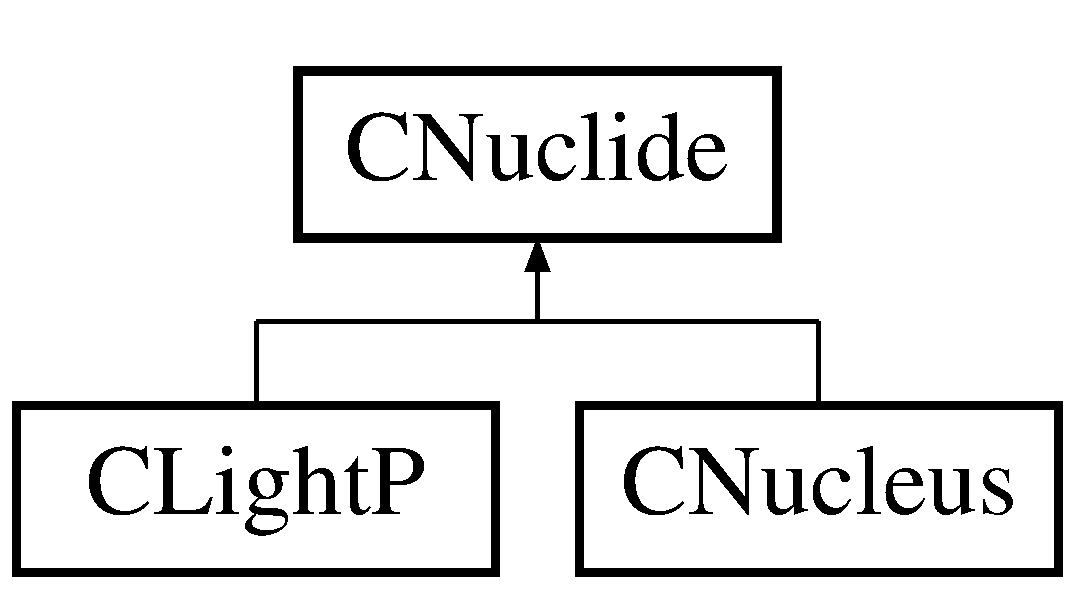
\includegraphics[height=2cm]{classCNuclide}
\end{center}
\end{figure}
\subsection*{Public Member Functions}
\begin{CompactItemize}
\item 
\bf{CNuclide} (int \bf{i\-Z}, int \bf{i\-A})
\item 
\bf{CNuclide} (int, int, string)
\item 
void \bf{init} (int, int)
\item 
float \bf{get\-Excess\-Mass} ()
\item 
const char $\ast$ \bf{get\-Symbol} ()
\item 
string \bf{get\-Name} ()
\end{CompactItemize}
\subsection*{Public Attributes}
\begin{CompactItemize}
\item 
\bf{CMass} $\ast$ \bf{mass}\label{classCNuclide_e020aeb91f8b7c73332082282cca3961}

\begin{CompactList}\small\item\em mass excess class \item\end{CompactList}\item 
\bf{CRandom} $\ast$ \bf{ran}\label{classCNuclide_077a728b5db1496bd6d6431b6499bbb3}

\begin{CompactList}\small\item\em random number generator class \item\end{CompactList}\item 
int \bf{i\-Z}\label{classCNuclide_9442a34164e471af32a1efe2a73068ea}

\begin{CompactList}\small\item\em proton number \item\end{CompactList}\item 
int \bf{i\-N}\label{classCNuclide_4eef1a690423544d82155b56597cd3d1}

\begin{CompactList}\small\item\em neutron number \item\end{CompactList}\item 
int \bf{i\-A}\label{classCNuclide_07b50da4719f3ab76d904561db2dca2e}

\begin{CompactList}\small\item\em mass number \item\end{CompactList}\item 
float \bf{f\-J}\label{classCNuclide_1365035203a9bc504512037f9e92efb8}

\begin{CompactList}\small\item\em spin [hbar] \item\end{CompactList}\item 
float \bf{f\-Exp\-Mass}\label{classCNuclide_7d8baf278610bc42f045b6332a394b34}

\begin{CompactList}\small\item\em mass excess [Me\-V] \item\end{CompactList}\item 
float \bf{f\-Ex}\label{classCNuclide_33f3a6977a3ac4e8451d11b2821e8c71}

\begin{CompactList}\small\item\em excitation energy [Me\-V] \item\end{CompactList}\end{CompactItemize}
\subsection*{Protected Attributes}
\begin{CompactItemize}
\item 
string \bf{str\-Chem\-Name}\label{classCNuclide_9edb051b9b41a65aa3aef03522886a38}

\begin{CompactList}\small\item\em gives isotopes and chemical name, e.g. 208Pb \item\end{CompactList}\item 
string \bf{str\-Name}\label{classCNuclide_9d3b5dd7382e7fb746ab7064243b3a5f}

\begin{CompactList}\small\item\em identifation name \item\end{CompactList}\end{CompactItemize}
\subsection*{Static Protected Attributes}
\begin{CompactItemize}
\item 
static const char $\ast$ \bf{name} [101]
\begin{CompactList}\small\item\em array containing name of all elements \item\end{CompactList}\end{CompactItemize}


\subsection{Detailed Description}
info on each nucleus 

!

basic class \doxyref{CNuclide}{p.}{classCNuclide} - stores the basic properties of the nucleus 



\subsection{Constructor \& Destructor Documentation}
\index{CNuclide@{CNuclide}!CNuclide@{CNuclide}}
\index{CNuclide@{CNuclide}!CNuclide@{CNuclide}}
\subsubsection{\setlength{\rightskip}{0pt plus 5cm}CNuclide::CNuclide (int {\em i\-Z0}, int {\em i\-A0})}\label{classCNuclide_5de0ac220b6cd6f177e9109bfac18934}


Constructor specifies the isotope \begin{Desc}
\item[Parameters:]
\begin{description}
\item[{\em i\-Z0}]is the proton number \item[{\em i\-A0}]is the mass number \end{description}
\end{Desc}
\index{CNuclide@{CNuclide}!CNuclide@{CNuclide}}
\index{CNuclide@{CNuclide}!CNuclide@{CNuclide}}
\subsubsection{\setlength{\rightskip}{0pt plus 5cm}CNuclide::CNuclide (int {\em i\-Z0}, int {\em i\-A0}, string {\em str\-Name0})}\label{classCNuclide_f89e1585817978cccb4270f51ec7fce1}


alternative constructor 

\subsection{Member Function Documentation}
\index{CNuclide@{CNuclide}!getExcessMass@{getExcessMass}}
\index{getExcessMass@{getExcessMass}!CNuclide@{CNuclide}}
\subsubsection{\setlength{\rightskip}{0pt plus 5cm}float CNuclide::get\-Excess\-Mass ()}\label{classCNuclide_9fbbaca94a94a919d220997451e47032}


Returns the excess mass of the nuclide \index{CNuclide@{CNuclide}!getName@{getName}}
\index{getName@{getName}!CNuclide@{CNuclide}}
\subsubsection{\setlength{\rightskip}{0pt plus 5cm}string CNuclide::get\-Name ()}\label{classCNuclide_a56693706f435a7bf3b45035e660d8d6}


Returns the chemical name of the isotope as a string \index{CNuclide@{CNuclide}!getSymbol@{getSymbol}}
\index{getSymbol@{getSymbol}!CNuclide@{CNuclide}}
\subsubsection{\setlength{\rightskip}{0pt plus 5cm}const char $\ast$ CNuclide::get\-Symbol ()}\label{classCNuclide_19999965219e259f915e9d49d628560e}


Returns the chemical name of the isotope as a character string \index{CNuclide@{CNuclide}!init@{init}}
\index{init@{init}!CNuclide@{CNuclide}}
\subsubsection{\setlength{\rightskip}{0pt plus 5cm}void CNuclide::init (int {\em i\-Z0}, int {\em i\-A0})}\label{classCNuclide_f0b72d479871636abab068355b6910df}


Initializes the isotope

Can be used to change the isotope \begin{Desc}
\item[Parameters:]
\begin{description}
\item[{\em i\-Z0}]is the proton number \item[{\em i\-A0}]is the mass number \end{description}
\end{Desc}


\subsection{Member Data Documentation}
\index{CNuclide@{CNuclide}!name@{name}}
\index{name@{name}!CNuclide@{CNuclide}}
\subsubsection{\setlength{\rightskip}{0pt plus 5cm}const char $\ast$ \bf{CNuclide::name}\hspace{0.3cm}{\tt  [static, protected]}}\label{classCNuclide_4cf136b7c82e01e82db1073690c2d355}


\textbf{Initial value:}

\begin{Code}\begin{verbatim}{"n","H","He","Li","Be","B",
                              "C","N","O","F","Ne",
                              "Na","Mg","Al","Si","P","S","Cl","Ar","K","Ca",
                              "Sc","Ti","V","Cr","Mn","Fe","Co","Ni","Cu","Zn",
                              "Ga","Ge","As","Se","Br","Kr","Rb","Sr","Y","Zr",
                              "Nb","Mo","Tc","Ru","Rh","Pd","Ag","Cd","In",
                              "Sn","Sb","Te","I","Xe","Cs","Ba","La","Ce","Pr",
                              "Nd","Pm","Sm","Eu","Gd","Tb","Dy","Ho","Er",
                               "Tm","Yb","Lu","Hf","Ta","W","Re","Os","Ir",
                              "Pt","Au","Hg","Tl","Pb","Bi","Po","At","Rn",
                              "Fr","Ra","Ac","Th","Pa","U","Np","Pu","Am",
                              "Cm","Bk","Cf","Es","Fm"}
\end{verbatim}\end{Code}
array containing name of all elements 



The documentation for this class was generated from the following files:\begin{CompactItemize}
\item 
CNuclide.h\item 
Nuclide.cpp\end{CompactItemize}

\section{CRandom Class Reference}
\label{classCRandom}\index{CRandom@{CRandom}}
Random numbers for a number of distributions.  


{\tt \#include $<$CRandom.h$>$}

\subsection*{Public Member Functions}
\begin{CompactItemize}
\item 
double \bf{Rndm} ()
\item 
float \bf{Gaus} (float mean, float sigma)
\item 
float \bf{exp\-Decay\-Time} (float width)
\item 
float \bf{Breit\-Wigner} (float mean, float width)
\end{CompactItemize}
\subsection*{Static Public Member Functions}
\begin{CompactItemize}
\item 
static \bf{CRandom} $\ast$ \bf{instance} ()
\begin{CompactList}\small\item\em instance member to make this a singleton \item\end{CompactList}\end{CompactItemize}
\subsection*{Protected Member Functions}
\begin{CompactItemize}
\item 
\bf{CRandom} ()
\end{CompactItemize}
\subsection*{Protected Attributes}
\begin{CompactItemize}
\item 
bool \bf{one}\label{classCRandom_0b76896418ae75089de37a3130e731bb}

\begin{CompactList}\small\item\em used for Gaus \item\end{CompactList}\item 
float \bf{angle}\label{classCRandom_3745da4f06cb91d7f74827976d33c348}

\begin{CompactList}\small\item\em used for Gaus \item\end{CompactList}\item 
float \bf{x}\label{classCRandom_976af97ef833bf86acf403f6227aa092}

\begin{CompactList}\small\item\em parameter \item\end{CompactList}\item 
float \bf{pi}\label{classCRandom_6cbe7ee72177c6c3052fd3756beb668f}

\begin{CompactList}\small\item\em 3.14159 \item\end{CompactList}\end{CompactItemize}
\subsection*{Static Protected Attributes}
\begin{CompactItemize}
\item 
static \bf{CRandom} $\ast$ \bf{f\-Instance} = 0\label{classCRandom_4f89b95eb9b92a92a03adabe5dfa9137}

\begin{CompactList}\small\item\em instance member to make tis a singleton \item\end{CompactList}\end{CompactItemize}


\subsection{Detailed Description}
Random numbers for a number of distributions. 

!

Random number generation using the C++ random number function 



\subsection{Constructor \& Destructor Documentation}
\index{CRandom@{CRandom}!CRandom@{CRandom}}
\index{CRandom@{CRandom}!CRandom@{CRandom}}
\subsubsection{\setlength{\rightskip}{0pt plus 5cm}CRandom::CRandom ()\hspace{0.3cm}{\tt  [protected]}}\label{classCRandom_8d7c54478494c868271476b23bacbe2e}


COnstructor for \doxyref{CRandom}{p.}{classCRandom} 

\subsection{Member Function Documentation}
\index{CRandom@{CRandom}!BreitWigner@{BreitWigner}}
\index{BreitWigner@{BreitWigner}!CRandom@{CRandom}}
\subsubsection{\setlength{\rightskip}{0pt plus 5cm}float CRandom::Breit\-Wigner (float {\em mean}, float {\em width})}\label{classCRandom_884f885e1cf081106f27a8ea25f14362}


Returns a random number with a Breit\-Wigner distribution \begin{Desc}
\item[Parameters:]
\begin{description}
\item[{\em mean}]is the mean value of the distribution \item[{\em width}]is the Full Width Half max of the distribution \end{description}
\end{Desc}
\index{CRandom@{CRandom}!expDecayTime@{expDecayTime}}
\index{expDecayTime@{expDecayTime}!CRandom@{CRandom}}
\subsubsection{\setlength{\rightskip}{0pt plus 5cm}float CRandom::exp\-Decay\-Time (float {\em width})}\label{classCRandom_26e937ca66f6b0b9163d6c63b8c902db}


returns a decay time in zs sampled from a exponential distribution \begin{Desc}
\item[Parameters:]
\begin{description}
\item[{\em width}]is the total decay width in Me\-V \end{description}
\end{Desc}
\index{CRandom@{CRandom}!Gaus@{Gaus}}
\index{Gaus@{Gaus}!CRandom@{CRandom}}
\subsubsection{\setlength{\rightskip}{0pt plus 5cm}float CRandom::Gaus (float {\em mean}, float {\em sigma})}\label{classCRandom_2ef2778f16be94f6d402949f05ee1318}


Returns random number with Gaussian distribution \begin{Desc}
\item[Parameters:]
\begin{description}
\item[{\em mean}]is the mean value of the Gaussian distribution \item[{\em sigma}]is the standard deviation of the distribution \end{description}
\end{Desc}
\index{CRandom@{CRandom}!instance@{instance}}
\index{instance@{instance}!CRandom@{CRandom}}
\subsubsection{\setlength{\rightskip}{0pt plus 5cm}\bf{CRandom} $\ast$ CRandom::instance ()\hspace{0.3cm}{\tt  [static]}}\label{classCRandom_f5d0eb4a4d10fb94151b9e6664b136f2}


instance member to make this a singleton 

Makes an instance of \doxyref{CRandom}{p.}{classCRandom} \index{CRandom@{CRandom}!Rndm@{Rndm}}
\index{Rndm@{Rndm}!CRandom@{CRandom}}
\subsubsection{\setlength{\rightskip}{0pt plus 5cm}double CRandom::Rndm ()}\label{classCRandom_d076a768bd120ebd05b71afe729692b9}


Returns a random number with uniform distribution between 0 and 1 

The documentation for this class was generated from the following files:\begin{CompactItemize}
\item 
CRandom.h\item 
Random.cpp\end{CompactItemize}

\section{CRun Class Reference}
\label{classCRun}\index{CRun@{CRun}}
example of fusion with root histograms  


{\tt \#include $<$CRun.h$>$}

\subsection*{Public Member Functions}
\begin{CompactItemize}
\item 
\textbf{CRun} (int i\-Z, int i\-A, float f\-Ex, float l0, float d0, int lmax, float plb, int num\-Tot, string title0, float vcm=0., float theta\-Det\-Min=0., float theta\-Det\-Max=360.)\label{classCRun_01e26f72913747034ef1d2f76f3b70f7}

\end{CompactItemize}


\subsection{Detailed Description}
example of fusion with root histograms 

!

class that I use to simulate statistical decay in fusion reaction. It produces a number of histograms, such a mass, charge and evaporation spectra - The output is stored in root file 



The documentation for this class was generated from the following file:\begin{CompactItemize}
\item 
CRun.h\end{CompactItemize}

\section{CRun\-Thick Class Reference}
\label{classCRunThick}\index{CRunThick@{CRunThick}}
example of fusion with root histograms  


{\tt \#include $<$CRun\-Thick.h$>$}

\subsection*{Public Member Functions}
\begin{CompactItemize}
\item 
\textbf{CRun\-Thick} (int i\-Z, int i\-A, float f\-Ex\_\-min, float f\-Ex\_\-max, float l0\_\-min, float l0\_\-Max, float d0, int lmax, float plb, int n\-Bins, int num\-Tot, string title0, float vcm=0., float theta\-Det\-Min=0., float theta\-Det\-Max=360.)\label{classCRunThick_e3d2dd1c5910701d1859181a67036be0}

\end{CompactItemize}


\subsection{Detailed Description}
example of fusion with root histograms 

!

class that I use to simulate statistical decay in fusion reactions where there is a thick target. It produces a number of histograms, such a mass, charge and evaporation spectra - The output is stored in root file 



The documentation for this class was generated from the following file:\begin{CompactItemize}
\item 
CRun\-Thick.h\end{CompactItemize}

\section{CScission Class Reference}
\label{classCScission}\index{CScission@{CScission}}
scission energies  


{\tt \#include $<$CScission.h$>$}

\subsection*{Public Member Functions}
\begin{CompactItemize}
\item 
\bf{CScission} (int i\-Z0, int i\-A0, float f\-J0, int i\-Chan)
\item 
\bf{CScission} ()
\item 
void \bf{init} (int i\-Z0, int i\-A0, float f\-J0, int ichan, float \bf{Z1}=0., float \bf{A1}=0.)
\item 
float \bf{get\-Sep} (float Ek\-Viola)
\item 
float \bf{get\-Scission\-Energy} ()
\item 
float \bf{get\-Scission\-Energy} (int i\-Z1, int i\-A1)
\item 
float \bf{get\-Fission\-Kinetic\-Energy} (int i\-Z1, int i\-A1)
\item 
float \bf{sigma\-Fission\-Systematics\-Scission} (int \bf{i\-Z}, int \bf{i\-A}, float \bf{f\-J}, float f\-Uscission)
\item 
float \bf{sigma\-Fission\-Systematics\-Saddle} (int \bf{i\-Z}, int \bf{i\-A}, float \bf{f\-J}, float f\-Uscission)
\end{CompactItemize}
\subsection*{Public Attributes}
\begin{CompactItemize}
\item 
float \bf{sep}\label{classCScission_7e0a0a9b1be469e17052698c3bb7e5c3}

\begin{CompactList}\small\item\em separation between the surafces of the 2 spheres \item\end{CompactList}\item 
float \bf{sep0}\label{classCScission_476acc48d1bb450aeb2277b4b19af0de}

\begin{CompactList}\small\item\em separation determined in \doxyref{init()}{p.}{classCScission_0c2bd3f431a6385d8bce851f49284ae8} \item\end{CompactList}\item 
float \bf{sep1}\label{classCScission_95ede779e290b86fe960b120001b899c}

\begin{CompactList}\small\item\em separation determined in sigma\-Fission\-Systematics() \item\end{CompactList}\item 
int \bf{i\-A}\label{classCScission_b468c2769bc37ebe21918a87057a07ff}

\begin{CompactList}\small\item\em mass number of system \item\end{CompactList}\item 
int \bf{i\-Z}\label{classCScission_1c611f244f8e8f6094570f529e3e084c}

\begin{CompactList}\small\item\em proton number of system \item\end{CompactList}\item 
float \bf{A}\label{classCScission_0120018c3a218a5615eefb199390ab31}

\begin{CompactList}\small\item\em float value of i\-A \item\end{CompactList}\item 
float \bf{Z}\label{classCScission_f817f8c63a13f4844770e3553336e56f}

\begin{CompactList}\small\item\em float value of i\-Z \item\end{CompactList}\item 
float \bf{f\-J}\label{classCScission_b10764ede0c5ee1c0269701c1a34d195}

\begin{CompactList}\small\item\em spin of system \item\end{CompactList}\item 
float \bf{Esymmetric}\label{classCScission_838a72a6358a91630362b136eff830ae}

\begin{CompactList}\small\item\em energy for symmetric mass split \item\end{CompactList}\item 
float \bf{ek\-Tot}\label{classCScission_7d2335cb14f3ab025a8899eb714f2264}

\begin{CompactList}\small\item\em total fission kinetic energy from \doxyref{get\-Fission\-Kinetic\-Energy()}{p.}{classCScission_41ffe401a64b471f3f6886ae42034486} \item\end{CompactList}\item 
float \bf{Erotate1}\label{classCScission_8ca6f7ca00675838a93349e5ebca605f}

\begin{CompactList}\small\item\em rotational energy of fragment1 \item\end{CompactList}\item 
float \bf{Erotate2}\label{classCScission_78e46526b068360b332ac6d4070dc3cc}

\begin{CompactList}\small\item\em rotational energy of fragment2 \item\end{CompactList}\item 
float \bf{Epair1}\label{classCScission_0808896a03852c1587ef84be24f704e3}

\begin{CompactList}\small\item\em pairing energy of frag1 \item\end{CompactList}\item 
float \bf{Epair2}\label{classCScission_1ff3a0893bf14ac980307b9bb3fc7c1c}

\begin{CompactList}\small\item\em pairing energy of frag2 \item\end{CompactList}\item 
float \bf{Eshell1}\label{classCScission_b95a595aebdd0686a86a1bc32a8994e8}

\begin{CompactList}\small\item\em shell energy of frag1 \item\end{CompactList}\item 
float \bf{Eshell2}\label{classCScission_50cf98780b0656cec97ec17711fe3cff}

\begin{CompactList}\small\item\em shell energy of frag2 \item\end{CompactList}\item 
float \bf{Ek\-Coul}\label{classCScission_16817cd0ceead5160405faf3fd47a774}

\begin{CompactList}\small\item\em Colomb part of total fisison kinetic energy. \item\end{CompactList}\item 
float \bf{Ek\-Rot}\label{classCScission_e26c54db91eeab7101e8b7aa409c9f22}

\begin{CompactList}\small\item\em rotational part of total fission kinetic energy \item\end{CompactList}\end{CompactItemize}
\subsection*{Static Public Attributes}
\begin{CompactItemize}
\item 
static float const \bf{r0} = 1.2\label{classCScission_2f0ac2f074774fd8ca26c7899eb48e51}

\begin{CompactList}\small\item\em constant R=r0$\ast$A$^\wedge$(1/3) \item\end{CompactList}\end{CompactItemize}
\subsection*{Protected Attributes}
\begin{CompactItemize}
\item 
float \bf{mu0}\label{classCScission_1d131cea4a4271de1eb070d3c4330993}

\begin{CompactList}\small\item\em reduced mass \item\end{CompactList}\item 
float \bf{Vc0}\label{classCScission_8872d25c5becefcdf2d90e8b5681be84}

\begin{CompactList}\small\item\em Coulomb self energy of a symmetric frag. \item\end{CompactList}\item 
float \bf{R1}\label{classCScission_5b059301c628acad5705a89980ab5fa1}

\begin{CompactList}\small\item\em radius of frag1 in fm \item\end{CompactList}\item 
float \bf{mom\-Inertia1}\label{classCScission_7e00010dcc73baff0d6b5caacf2eec65}

\begin{CompactList}\small\item\em moment of inertia of frgament1 \item\end{CompactList}\item 
float \bf{R2}\label{classCScission_80f047e282b797b42216a88de9382485}

\begin{CompactList}\small\item\em radius of frag1 in fm \item\end{CompactList}\item 
float \bf{mom\-Inertia2}\label{classCScission_fcbcfbb41e547ca414b487e5b15c685d}

\begin{CompactList}\small\item\em moment of inertia of frgament1 \item\end{CompactList}\item 
float \bf{k1}\label{classCScission_762eeaf7126c455d8cf8be26f057d79f}

\begin{CompactList}\small\item\em part of the rotational energy \item\end{CompactList}\item 
bool \bf{sym}\label{classCScission_2030b52f9a5a46f4898c4cdde7949155}

\begin{CompactList}\small\item\em logical symmetic of non symmetric fission \item\end{CompactList}\item 
float \bf{Z1}\label{classCScission_c28f0da8de7c21d16c1a2a90859ee418}

\begin{CompactList}\small\item\em atomic number of lighter fragment after fission \item\end{CompactList}\item 
float \bf{Z2}\label{classCScission_f4da998a5bb98b7cdc157d26b0cb86a4}

\begin{CompactList}\small\item\em atomic number of heavier fragment \item\end{CompactList}\item 
float \bf{A1}\label{classCScission_325801d1f2d4f3cee12df6dff0c7edb7}

\begin{CompactList}\small\item\em mass number of lighter fragment after fission \item\end{CompactList}\item 
float \bf{A2}\label{classCScission_ba0abbfdc704b9d5198bb6e006383f99}

\begin{CompactList}\small\item\em mass number of heavier fragment \item\end{CompactList}\item 
\bf{CMass} $\ast$ \bf{mass}\label{classCScission_fac372a82d76862c75c3b2d5a8dc2e7f}

\begin{CompactList}\small\item\em gives mass excess \item\end{CompactList}\end{CompactItemize}
\subsection*{Static Protected Attributes}
\begin{CompactItemize}
\item 
static float const \bf{e2} = 1.44\label{classCScission_a379552dc524c1769dfa4524156ac2bb}

\begin{CompactList}\small\item\em $e^{2} = 1.44 MeV fm^{-1}$ \item\end{CompactList}\item 
static float const \bf{k\-Rotate} = 41.563\label{classCScission_8306f38f83714310050a33b91acdd630}

\begin{CompactList}\small\item\em constant for rotational energy \item\end{CompactList}\item 
static float const \bf{slope\-Viola} = .1189\label{classCScission_50aab84021ddc5fdb54347e744d4bf5e}

\begin{CompactList}\small\item\em for Viola systematics of fission KE \item\end{CompactList}\item 
static float const \bf{const\-Viola} = 7.3\label{classCScission_5095de5115a5480935cb7dce78942b56}

\begin{CompactList}\small\item\em for Viola systematics of fission KE \item\end{CompactList}\end{CompactItemize}


\subsection{Detailed Description}
scission energies 

!

calculates information on scission point for saddle-to-scission evaporation and for fission mass distributions 



\subsection{Constructor \& Destructor Documentation}
\index{CScission@{CScission}!CScission@{CScission}}
\index{CScission@{CScission}!CScission@{CScission}}
\subsubsection{\setlength{\rightskip}{0pt plus 5cm}CScission::CScission (int {\em i\-Z0}, int {\em i\-A0}, float {\em f\-J0}, int {\em i\-Chan})}\label{classCScission_538659c740716a9a6124fa331e599aaf}


constructor /param i\-Z0 is proton number of fissioning nucleus /param i\-A0 is mass number of fission nucleus /param f\-J0 is spin of fissioning nucleus /param i\-Chan =1 for imf, =2 symmetric fission \index{CScission@{CScission}!CScission@{CScission}}
\index{CScission@{CScission}!CScission@{CScission}}
\subsubsection{\setlength{\rightskip}{0pt plus 5cm}CScission::CScission ()}\label{classCScission_24857c87fd9bc9c6d1f6d075e89e4ded}


simple constructor 

\subsection{Member Function Documentation}
\index{CScission@{CScission}!getFissionKineticEnergy@{getFissionKineticEnergy}}
\index{getFissionKineticEnergy@{getFissionKineticEnergy}!CScission@{CScission}}
\subsubsection{\setlength{\rightskip}{0pt plus 5cm}float CScission::get\-Fission\-Kinetic\-Energy (int {\em i\-Z1}, int {\em i\-A1})}\label{classCScission_41ffe401a64b471f3f6886ae42034486}


returns the total fission kinetic energy from a two sphere approximation using the separation sep determined from either \doxyref{init()}{p.}{classCScission_0c2bd3f431a6385d8bce851f49284ae8} to sigma\-Fission\-Systematics(), whichever was called last /param i\-Z1 is the proton number of one of the fragments /param i\-Z2 is the mass number of one of the fragments \index{CScission@{CScission}!getScissionEnergy@{getScissionEnergy}}
\index{getScissionEnergy@{getScissionEnergy}!CScission@{CScission}}
\subsubsection{\setlength{\rightskip}{0pt plus 5cm}float CScission::get\-Scission\-Energy (int {\em i\-Z1}, int {\em i\-A1})}\label{classCScission_1b5c552ee7cbf5a07b8d2d4af059eaf6}


returns the asymmetric fission scission energy from a two sphere approximation using the separation sep previously determined from \doxyref{init()}{p.}{classCScission_0c2bd3f431a6385d8bce851f49284ae8} to sigma\-Fission\-Systematics() /param i\-Z1 is the proton number of one of the fission fragments /param i\-A1 is the mass number of one of the fission fragments \index{CScission@{CScission}!getScissionEnergy@{getScissionEnergy}}
\index{getScissionEnergy@{getScissionEnergy}!CScission@{CScission}}
\subsubsection{\setlength{\rightskip}{0pt plus 5cm}float CScission::get\-Scission\-Energy ()}\label{classCScission_e6bcb5439e5a29fdf98819761bbddc73}


returns the symmetric fission scission energy from a two sphere approximation using the separation sep previously determined from \doxyref{init()}{p.}{classCScission_0c2bd3f431a6385d8bce851f49284ae8} to sigma\-Fission\-Systematics \index{CScission@{CScission}!getSep@{getSep}}
\index{getSep@{getSep}!CScission@{CScission}}
\subsubsection{\setlength{\rightskip}{0pt plus 5cm}float CScission::get\-Sep (float {\em ek\-Viola})}\label{classCScission_bdbff203a89a1233fc8345603e5edd17}


approximates the scission configuration by two separated spheres. returns the separation between the surface of the sphere which is consistent with input fission total kinetic energy /param ek\-Viola is the total fission kinetic energy \index{CScission@{CScission}!init@{init}}
\index{init@{init}!CScission@{CScission}}
\subsubsection{\setlength{\rightskip}{0pt plus 5cm}void CScission::init (int {\em i\-Z0}, int {\em i\-A0}, float {\em f\-J0}, int {\em i\-Chan}, float {\em Z10} = {\tt 0.}, float {\em A10} = {\tt 0.})}\label{classCScission_0c2bd3f431a6385d8bce851f49284ae8}


initialized the calls for a given nucleus /param i\-Z0 is the proton number of the nucleus /param i\-A0 is the mass number of the nucleus /param f\-J0 is the spin of the nucleus /param i\-Chan =1 for imf, =2 symmetric fission \index{CScission@{CScission}!sigmaFissionSystematicsSaddle@{sigmaFissionSystematicsSaddle}}
\index{sigmaFissionSystematicsSaddle@{sigmaFissionSystematicsSaddle}!CScission@{CScission}}
\subsubsection{\setlength{\rightskip}{0pt plus 5cm}float CScission::sigma\-Fission\-Systematics\-Saddle (int {\em i\-Z0}, int {\em i\-A0}, float {\em f\-J}, float {\em f\-UScission})}\label{classCScission_3fae208f820a708db985e456187be82b}


estimates the standard deviation of the fission mass distributions from the systematics of Rusanov et al. Physics of the Atomic Nucleus 60 (1997) 683 assuming a saddle-point logic. subsequentally, it approximates the scission configuration as two separated spheres, where the separation is adjusted to reproduce the mass distribution \begin{Desc}
\item[Parameters:]
\begin{description}
\item[{\em i\-Z0}]is the proton number \item[{\em i\-A0}]is the mass number \item[{\em f\-J}]is the angular momentum \item[{\em f\-UScission}]is the thermal excitation energy at the scission-point in Me\-V \end{description}
\end{Desc}
\index{CScission@{CScission}!sigmaFissionSystematicsScission@{sigmaFissionSystematicsScission}}
\index{sigmaFissionSystematicsScission@{sigmaFissionSystematicsScission}!CScission@{CScission}}
\subsubsection{\setlength{\rightskip}{0pt plus 5cm}float CScission::sigma\-Fission\-Systematics\-Scission (int {\em i\-Z0}, int {\em i\-A0}, float {\em f\-J}, float {\em f\-UScission})}\label{classCScission_d4d8f6ddbac1668d6849c3a0cd51840e}


estimates the standard deviation of the fission mass distributions from the systematics of Rusanov et al. Physics of the Atomic Nucleus 60 (1997) 683 assuming a scission-point logic. subsequentally, it approximates the scission configuration as two separated spheres, where the separation is adjusted to reproduce the mass distribution \begin{Desc}
\item[Parameters:]
\begin{description}
\item[{\em i\-Z0}]is the proton number \item[{\em i\-A0}]is the mass number \item[{\em f\-J}]is the angular momentum \item[{\em f\-UScission}]is the thermal excitation energy at the scission-point in Me\-V \end{description}
\end{Desc}


The documentation for this class was generated from the following files:\begin{CompactItemize}
\item 
CScission.h\item 
Scission.cpp\end{CompactItemize}

\section{CSig\-Bar\-Dist Class Reference}
\label{classCSigBarDist}\index{CSigBarDist@{CSigBarDist}}
inverse cross section with barrier distributions  


{\tt \#include $<$CSig\-Bar\-Dist.h$>$}

\subsection*{Public Member Functions}
\begin{CompactItemize}
\item 
\bf{CSig\-Bar\-Dist} (string, float Zp0, float Ap0)
\item 
\bf{$\sim$CSig\-Bar\-Dist} ()
\item 
float \bf{get\-Inverse\-Xsec} (float f\-Ek, float temp)
\item 
void \bf{prepare} (float \bf{Z}, float \bf{A})
\item 
float \bf{get\-Barrier} ()
\end{CompactItemize}
\subsection*{Static Public Member Functions}
\begin{CompactItemize}
\item 
static void \bf{set\-Bar\-Width} (float width00)
\item 
static float \bf{get\-Bar\-Width} ()
\item 
static void \bf{print\-Parameters} ()
\end{CompactItemize}
\subsection*{Private Attributes}
\begin{CompactItemize}
\item 
\bf{CSig\-Charged} $\ast$ \bf{sig\-Charged} [3]\label{classCSigBarDist_5e86ed64783828fa440859e380b1d1da}

\begin{CompactList}\small\item\em arrays for standard radii and +- width0 \item\end{CompactList}\item 
bool \bf{one}\label{classCSigBarDist_61ce73d84bfda0b0d2d29c85fb5b20fd}

\begin{CompactList}\small\item\em if true, no distribution, just standard radius is used \item\end{CompactList}\item 
float \bf{Z}\label{classCSigBarDist_9a9699ea3c6cd8270ed564c136c5007a}

\begin{CompactList}\small\item\em calls to get\-Inverse\-Xsec refer to this residual proton number \item\end{CompactList}\item 
float \bf{A}\label{classCSigBarDist_20659289535a2d303e39aff96e957ff9}

\begin{CompactList}\small\item\em calls to get\-Inverse\-Xsec refer to this residual mass number \item\end{CompactList}\item 
float \bf{Zp}\label{classCSigBarDist_257fd637d8c84837cb7df124d26c7bc0}

\begin{CompactList}\small\item\em proton number of evaporated particle \item\end{CompactList}\item 
float \bf{Ap}\label{classCSigBarDist_901d950d11630943e11749fc21cbeeb3}

\begin{CompactList}\small\item\em mass number of evaporated particle \item\end{CompactList}\end{CompactItemize}
\subsection*{Static Private Attributes}
\begin{CompactItemize}
\item 
static float \bf{width} = 1.\label{classCSigBarDist_07e67e476a5452df83f9a348ab8a23c8}

\begin{CompactList}\small\item\em width paramter determines shifted radii \item\end{CompactList}\item 
static float const \bf{width0} = 1.5\label{classCSigBarDist_9bbbb75c2633d7dbad4e5e85264636d1}

\begin{CompactList}\small\item\em results readin from file for this shift \item\end{CompactList}\end{CompactItemize}


\subsection{Detailed Description}
inverse cross section with barrier distributions 

!

calculates transmission coefficientinverse cross sections using a simplistic barrier distribution logic. The final result is the average of three inverse cross sections. $ T_{l}(Ek) = \frac{T_{l}^{R_{0}-\Delta R}(Ek) + T_{l}^{R_{0}}(Ek) + T_{l}^{R_{0}+\Delta R}(Ek)}{3} $ where $ T_{l}^{R_{0}}$ is the standard coeff derived using the IWBC and global optical-model potential. The other two are for when the radius of the nuclear potential is shifted by $ \pm \Delta R $. where $ \Delta R = width*\sqrt{temperature} $. 



\subsection{Constructor \& Destructor Documentation}
\index{CSigBarDist@{CSig\-Bar\-Dist}!CSigBarDist@{CSigBarDist}}
\index{CSigBarDist@{CSigBarDist}!CSigBarDist@{CSig\-Bar\-Dist}}
\subsubsection{\setlength{\rightskip}{0pt plus 5cm}CSig\-Bar\-Dist::CSig\-Bar\-Dist (string {\em s\-Name0}, float {\em Zp0}, float {\em Ap0})}\label{classCSigBarDist_5fef91947df17b399099110d91b42529}


constructor /param s\-Name0 is the name of the files containing fitted coeff. \index{CSigBarDist@{CSig\-Bar\-Dist}!~CSigBarDist@{$\sim$CSigBarDist}}
\index{~CSigBarDist@{$\sim$CSigBarDist}!CSigBarDist@{CSig\-Bar\-Dist}}
\subsubsection{\setlength{\rightskip}{0pt plus 5cm}CSig\-Bar\-Dist::$\sim$CSig\-Bar\-Dist ()}\label{classCSigBarDist_bf984b4157ee3f414f683e6e5187b7e9}


destructor 

\subsection{Member Function Documentation}
\index{CSigBarDist@{CSig\-Bar\-Dist}!getBarrier@{getBarrier}}
\index{getBarrier@{getBarrier}!CSigBarDist@{CSig\-Bar\-Dist}}
\subsubsection{\setlength{\rightskip}{0pt plus 5cm}float CSig\-Bar\-Dist::get\-Barrier ()}\label{classCSigBarDist_fca88f547fd3cdd8901b6e4ad27726c3}


returns the barrier in Me\-V \index{CSigBarDist@{CSig\-Bar\-Dist}!getBarWidth@{getBarWidth}}
\index{getBarWidth@{getBarWidth}!CSigBarDist@{CSig\-Bar\-Dist}}
\subsubsection{\setlength{\rightskip}{0pt plus 5cm}float CSig\-Bar\-Dist::get\-Bar\-Width ()\hspace{0.3cm}{\tt  [static]}}\label{classCSigBarDist_52ec33821f2367cf05eb72d052c01d88}


returns the parameter controlling the width of the barrier dist \index{CSigBarDist@{CSig\-Bar\-Dist}!getInverseXsec@{getInverseXsec}}
\index{getInverseXsec@{getInverseXsec}!CSigBarDist@{CSig\-Bar\-Dist}}
\subsubsection{\setlength{\rightskip}{0pt plus 5cm}float CSig\-Bar\-Dist::get\-Inverse\-Xsec (float {\em f\-Ek}, float {\em temp})}\label{classCSigBarDist_208b57a94504830b93649c2927ce39f1}


returns the quantity $S=\sum_{\ell=0}^{\infty} (2\ell+1)T_{\ell}(\varepsilon)$ which is related to the inverse cross section by $S=\frac{\sigma_{inv}}{\pi\lambda^{2}}$ \begin{Desc}
\item[Parameters:]
\begin{description}
\item[{\em f\-Ek}]is the kinetic energy of the evaporated particle \item[{\em temp}]is temperature of daughter in Me\-V \end{description}
\end{Desc}
\index{CSigBarDist@{CSig\-Bar\-Dist}!prepare@{prepare}}
\index{prepare@{prepare}!CSigBarDist@{CSig\-Bar\-Dist}}
\subsubsection{\setlength{\rightskip}{0pt plus 5cm}void CSig\-Bar\-Dist::prepare (float {\em Z0}, float {\em A0})}\label{classCSigBarDist_d81bc66a58512cd7ab23bf10fc4ce7ca}


prepares for a series of opertions for a given i\-Z /param i\-Z0 is proton number of daughter \index{CSigBarDist@{CSig\-Bar\-Dist}!printParameters@{printParameters}}
\index{printParameters@{printParameters}!CSigBarDist@{CSig\-Bar\-Dist}}
\subsubsection{\setlength{\rightskip}{0pt plus 5cm}void CSig\-Bar\-Dist::print\-Parameters ()\hspace{0.3cm}{\tt  [static]}}\label{classCSigBarDist_18a63652d6600aae4ede085dcaf522f9}


prints out the width parameter \index{CSigBarDist@{CSig\-Bar\-Dist}!setBarWidth@{setBarWidth}}
\index{setBarWidth@{setBarWidth}!CSigBarDist@{CSig\-Bar\-Dist}}
\subsubsection{\setlength{\rightskip}{0pt plus 5cm}void CSig\-Bar\-Dist::set\-Bar\-Width (float {\em width00})\hspace{0.3cm}{\tt  [static]}}\label{classCSigBarDist_c2d8d22c9bf77a1988fa934201a40fd5}


set the parameter controlling the width of the barrier distribution \begin{Desc}
\item[Parameters:]
\begin{description}
\item[{\em width00}]- radial shift is $ \Delta R= \sqrt T* width00 $ \end{description}
\end{Desc}


The documentation for this class was generated from the following files:\begin{CompactItemize}
\item 
CSig\-Bar\-Dist.h\item 
Sig\-Bar\-Dist.cpp\end{CompactItemize}

\section{CSig\-Charged Class Reference}
\label{classCSigCharged}\index{CSigCharged@{CSigCharged}}
inverse xsections  


{\tt \#include $<$CSig\-Charged.h$>$}

\subsection*{Public Member Functions}
\begin{CompactItemize}
\item 
\bf{CSig\-Charged} (string file, float Zp0, float Ap0)\label{classCSigCharged_f1a0c7d0b39115a3da7ba80d35633461}

\begin{CompactList}\small\item\em constructor \item\end{CompactList}\item 
void \bf{prepare} (float Z, float A)\label{classCSigCharged_1ff354f15be674a0cf48be6a8c92362a}

\begin{CompactList}\small\item\em prepares for calculations of inverse xsections \item\end{CompactList}\item 
float \bf{get\-Inverse\-Xsec} (float energy)\label{classCSigCharged_481a8b2ee84c4a2394396fc1ff3830bc}

\begin{CompactList}\small\item\em calculates the inverse xsection \item\end{CompactList}\item 
float \bf{get\-Barrier} ()\label{classCSigCharged_229a7e136b539bfe31ae313497f029ac}

\begin{CompactList}\small\item\em calculates the barrier \item\end{CompactList}\end{CompactItemize}
\subsection*{Private Attributes}
\begin{CompactItemize}
\item 
string \bf{s\-Name}\label{classCSigCharged_01f9a1cab2ec8b56bb0793877bd60e2f}

\begin{CompactList}\small\item\em name of input file of coefficients \item\end{CompactList}\item 
float \bf{rc0}\label{classCSigCharged_2e9ec2ff0dcb3fb2c2bc9de795cf2d9f}

\begin{CompactList}\small\item\em paramter to calculate radius for Coulomb barrier \item\end{CompactList}\item 
float \bf{rc1}\label{classCSigCharged_95be4c57efdffcc3f3226a6f05eee5ef}

\begin{CompactList}\small\item\em paramter to calculate radius for Coulomb barrier \item\end{CompactList}\item 
float \bf{rc2}\label{classCSigCharged_0dcd5b2c790d16cb61f104f65d388894}

\begin{CompactList}\small\item\em paramter to calculate radius for Coulomb barrier \item\end{CompactList}\item 
float \bf{omega0}\label{classCSigCharged_68809d69d20bb519183353c3c906d00e}

\begin{CompactList}\small\item\em paramter for omega \item\end{CompactList}\item 
float \bf{omega1}\label{classCSigCharged_3c051766a9894adcad4e44b5ca32dcbc}

\begin{CompactList}\small\item\em parameter for omega \item\end{CompactList}\item 
float \bf{omega2}\label{classCSigCharged_a6c3fc42a9234e2e3a9c86e701b47ee8}

\begin{CompactList}\small\item\em parameter for omega \item\end{CompactList}\item 
float \bf{omega3}\label{classCSigCharged_12c9f21352794c01bcc43bc2e4b5bb39}

\begin{CompactList}\small\item\em parameter for omega \item\end{CompactList}\item 
float \bf{r\-I0}\label{classCSigCharged_1d80ea773c32a209e2a59ff2127bd79e}

\begin{CompactList}\small\item\em paramter for radius for rotational energy \item\end{CompactList}\item 
float \bf{r\-I1}\label{classCSigCharged_b48b08d3862b74bfa5747269d6356a63}

\begin{CompactList}\small\item\em paramter for radius for rotational energy \item\end{CompactList}\item 
float \bf{r\-I2}\label{classCSigCharged_da18f138bed0f3c8c27f2afaa3fed991}

\begin{CompactList}\small\item\em paramter for radius for rotational energy \item\end{CompactList}\item 
float \bf{aa0}\label{classCSigCharged_6b8879bfcbd5795f59e61e6df5b5d8e6}

\begin{CompactList}\small\item\em below barrier correction parameter \item\end{CompactList}\item 
float \bf{aa1}\label{classCSigCharged_48b8b25cfb0231e40f94a00da13e3c85}

\begin{CompactList}\small\item\em below barrier correction parameter \item\end{CompactList}\item 
float \bf{a0}\label{classCSigCharged_19668087e1a2b0760639a42b9e141caf}

\begin{CompactList}\small\item\em above barrier correction parameter \item\end{CompactList}\item 
float \bf{a1}\label{classCSigCharged_0f53eb037a0604ef46b9bcd8123bc47a}

\begin{CompactList}\small\item\em above barrier correction parameter \item\end{CompactList}\item 
float \bf{Zp}\label{classCSigCharged_af05329196a8ad846c52c84f8624d05e}

\begin{CompactList}\small\item\em proton number of evaporated particle \item\end{CompactList}\item 
float \bf{Ap}\label{classCSigCharged_3dbeea3317884d86f0b33fc2a0eb403c}

\begin{CompactList}\small\item\em mass number of evaporated particle \item\end{CompactList}\item 
float \bf{barrier}\label{classCSigCharged_93315540bc38507bc5e93fb4a5e2b9e8}

\begin{CompactList}\small\item\em Coulomb barrier in Me\-V. \item\end{CompactList}\item 
float \bf{Inv\-Inertia}\label{classCSigCharged_df7bc08f4b6389120a07f4db07a4edb7}

\begin{CompactList}\small\item\em inverse of the moment of inertia associated with rotateion \item\end{CompactList}\item 
float \bf{omega}\label{classCSigCharged_0a576694df692a880cfd39b99784fa30}

\begin{CompactList}\small\item\em amega parameter in Me\-V \item\end{CompactList}\item 
float \bf{a}\label{classCSigCharged_685b5e0fbca8bfdaf3e4f7eb20ec90a4}

\begin{CompactList}\small\item\em above barrier correction \item\end{CompactList}\item 
float \bf{aa}\label{classCSigCharged_aaba6b096eabd13e2b67d3280a3b5621}

\begin{CompactList}\small\item\em below barrier correction \item\end{CompactList}\item 
float \bf{offset}\label{classCSigCharged_eebf83c2154c3cf90e4d5bc542ebec5e}

\begin{CompactList}\small\item\em offset \item\end{CompactList}\item 
bool \bf{neutron}\label{classCSigCharged_ddd3529b64f4785ebed1c1c836014040}

\begin{CompactList}\small\item\em bool to signify neutron calculation \item\end{CompactList}\item 
float \bf{n0}\label{classCSigCharged_d963202b2a1cbe5ed6b32c13633f04cb}

\begin{CompactList}\small\item\em neutron parameter \item\end{CompactList}\item 
float \bf{n1}\label{classCSigCharged_9195bf8cbeca8cd04cb40b9bb9bf2314}

\begin{CompactList}\small\item\em neutron parameter \item\end{CompactList}\item 
float \bf{n2}\label{classCSigCharged_15d00779ea82f9e4d5343faeb2d8d6d5}

\begin{CompactList}\small\item\em neutron parameter \item\end{CompactList}\end{CompactItemize}


\subsection{Detailed Description}
inverse xsections 

!

This class calculates $ \sum_{0}^{\infty} (2\ell+1) T_{\ell}(\varepsilon)$ which is the inverse xsection divided by $ \pi/k^2 $ 



The documentation for this class was generated from the following files:\begin{CompactItemize}
\item 
CSig\-Charged.h\item 
Sig\-Charged.cpp\end{CompactItemize}

\section{CTl\-Array Class Reference}
\label{classCTlArray}\index{CTlArray@{CTlArray}}
IWBC transmission coefficients.  


{\tt \#include $<$CTl\-Array.h$>$}

\subsection*{Public Member Functions}
\begin{CompactItemize}
\item 
\bf{CTl\-Array} (string)
\item 
float \bf{get\-Term\-In\-Exp} (int i\-L, float f\-Ek)
\item 
void \bf{prepare} (int i\-Z)
\item 
float \bf{get\-Tl} (int i\-L, float f\-Ek)
\item 
float \bf{get\-Inverse\-Xsec} (float f\-Ek)
\end{CompactItemize}
\subsection*{Public Attributes}
\begin{CompactItemize}
\item 
int \bf{i\-ZMin}\label{classCTlArray_e3c9a7b0480c4bcff98f10970ed99051}

\begin{CompactList}\small\item\em the minimum Z-value for coefficinets are stored \item\end{CompactList}\end{CompactItemize}
\subsection*{Protected Attributes}
\begin{CompactItemize}
\item 
\bf{SZcoef} \bf{zcoef}\label{classCTlArray_5028ad63ebf842107ed442c414510abc}

\begin{CompactList}\small\item\em structure to store coefficients parametrizating Tl's \item\end{CompactList}\item 
string \bf{s\-Name}\label{classCTlArray_34cd39424a5bd64bd88c143d051e1ceb}

\begin{CompactList}\small\item\em name of file containg Tl parameters \item\end{CompactList}\item 
float \bf{shift}\label{classCTlArray_81585d8de22b732d853064f63d1105f2}

\begin{CompactList}\small\item\em energy shift used in the parametrization \item\end{CompactList}\item 
\bf{SAng\-Tl} $\ast$ \bf{trans}\label{classCTlArray_c052b5a65a2c6701f1bc7ad3a383a24b}

\begin{CompactList}\small\item\em pointer to coefficents for a select i\-Z \item\end{CompactList}\end{CompactItemize}


\subsection{Detailed Description}
IWBC transmission coefficients. 

!

Provides transmission coefficients and inverse cross sections for light-partice evaporation 



\subsection{Constructor \& Destructor Documentation}
\index{CTlArray@{CTl\-Array}!CTlArray@{CTlArray}}
\index{CTlArray@{CTlArray}!CTlArray@{CTl\-Array}}
\subsubsection{\setlength{\rightskip}{0pt plus 5cm}CTl\-Array::CTl\-Array (string {\em s\-Name0})}\label{classCTlArray_2da7e96c7b1c0e751799cc2efa35440e}


Constructor \begin{Desc}
\item[Parameters:]
\begin{description}
\item[{\em s\-Name0}]is the name of the $\ast$.tl file in directory /tl where the parameters specifying the transmission coefficents are contained \end{description}
\end{Desc}


\subsection{Member Function Documentation}
\index{CTlArray@{CTl\-Array}!getInverseXsec@{getInverseXsec}}
\index{getInverseXsec@{getInverseXsec}!CTlArray@{CTl\-Array}}
\subsubsection{\setlength{\rightskip}{0pt plus 5cm}float CTl\-Array::get\-Inverse\-Xsec (float {\em f\-Ek})}\label{classCTlArray_b9a9ae1a39619e3a2836b2001dcb39ba}


returns the quantity $S=\sum_{\ell=0}^{\infty} (2\ell+1)T_{\ell}(\varepsilon)$ which is related to the inverse cross section by $S=\frac{\sigma_{inv}}{\pi\lambda^{2}}$ \begin{Desc}
\item[Parameters:]
\begin{description}
\item[{\em f\-Ek}]is the kinetic energy of the evaporated particle \end{description}
\end{Desc}
\index{CTlArray@{CTl\-Array}!getTermInExp@{getTermInExp}}
\index{getTermInExp@{getTermInExp}!CTlArray@{CTl\-Array}}
\subsubsection{\setlength{\rightskip}{0pt plus 5cm}float CTl\-Array::get\-Term\-In\-Exp (int {\em i\-L}, float {\em f\-Ek})}\label{classCTlArray_b3722411ddf490b7057cd8df907bf559}


The transmission coeff are parameterized as $\frac{1}{1+exp(x)}$ this function returns the value of x \begin{Desc}
\item[Parameters:]
\begin{description}
\item[{\em i\-L}]is the orbital angular momentum of the evaporated particle \item[{\em f\-Ek}]is the kinetic energy of the evaporated particle \end{description}
\end{Desc}
\index{CTlArray@{CTl\-Array}!getTl@{getTl}}
\index{getTl@{getTl}!CTlArray@{CTl\-Array}}
\subsubsection{\setlength{\rightskip}{0pt plus 5cm}float CTl\-Array::get\-Tl (int {\em i\-L}, float {\em f\-Ek})}\label{classCTlArray_a8d48df48e1c635f88157c081500f893}


Returns the transmission coefficient \begin{Desc}
\item[Parameters:]
\begin{description}
\item[{\em i\-L}]is the orbital angular momentum of the evaporated particle \item[{\em f\-Ek}]is the kinetic energy of the evaporated particle \end{description}
\end{Desc}
\index{CTlArray@{CTl\-Array}!prepare@{prepare}}
\index{prepare@{prepare}!CTlArray@{CTl\-Array}}
\subsubsection{\setlength{\rightskip}{0pt plus 5cm}void CTl\-Array::prepare (int {\em i\-Z})}\label{classCTlArray_714f982512481d8d188ea536235d84b6}


prepares for a series of calls with the same Z value \begin{Desc}
\item[Parameters:]
\begin{description}
\item[{\em i\-Z}]is the proton number of the daughter \end{description}
\end{Desc}


The documentation for this class was generated from the following files:\begin{CompactItemize}
\item 
CTl\-Array.h\item 
Tl\-Array.cpp\end{CompactItemize}

\section{CTl\-Bar\-Dist Class Reference}
\label{classCTlBarDist}\index{CTlBarDist@{CTlBarDist}}
transmission coefficients with barrier distibution  


{\tt \#include $<$CTl\-Bar\-Dist.h$>$}

\subsection*{Public Member Functions}
\begin{CompactItemize}
\item 
\bf{CTl\-Bar\-Dist} (string)
\item 
\bf{$\sim$CTl\-Bar\-Dist} ()
\item 
float \bf{get\-Tl} (int i\-L, float f\-Ek, float temp)
\item 
float \bf{get\-Tl\-Low} (int i\-L, float f\-Ek, float temp)
\item 
float \bf{get\-Tl\-High} (int i\-L, float f\-Ek, float temp)
\item 
float \bf{get\-Inverse\-Xsec} (float f\-Ek, float temp)
\item 
void \bf{prepare} (int i\-Z0)
\end{CompactItemize}
\subsection*{Static Public Member Functions}
\begin{CompactItemize}
\item 
static void \bf{set\-Bar\-Width} (float width00)
\item 
static float \bf{get\-Bar\-Width} ()
\item 
static void \bf{print\-Parameters} ()
\end{CompactItemize}
\subsection*{Private Attributes}
\begin{CompactItemize}
\item 
\bf{CTl\-Array} $\ast$ \bf{tl\-Array} [3]\label{classCTlBarDist_b1b034052d1d891b283178cab3e02199}

\begin{CompactList}\small\item\em arrays for standard radii and +- width0 \item\end{CompactList}\item 
bool \bf{one}\label{classCTlBarDist_8ea42d0d19f5d9de689b55b02cd352b5}

\begin{CompactList}\small\item\em if true, no distribution, just standard radius is used \item\end{CompactList}\item 
int \bf{i\-Z}\label{classCTlBarDist_a0d1e4422f41890e116c37ea4b60bf61}

\begin{CompactList}\small\item\em calls to get\-Tl refer to this residual proton number \item\end{CompactList}\end{CompactItemize}
\subsection*{Static Private Attributes}
\begin{CompactItemize}
\item 
static float \bf{width} = 1.\label{classCTlBarDist_5c3f55537cedd466a5efc497b26f400f}

\begin{CompactList}\small\item\em width paramter determines shifted radii \item\end{CompactList}\item 
static float const \bf{width0} = 1.5\label{classCTlBarDist_9df6198d2b6b4801cba17daa1a000624}

\begin{CompactList}\small\item\em results readin from file for this shift \item\end{CompactList}\end{CompactItemize}


\subsection{Detailed Description}
transmission coefficients with barrier distibution 

!

calculates transmission coefficients using a simplistic barrier distribution logic. The final result is the average of three transmission coefficients. $ T_{l}(Ek) = \frac{T_{l}^{R_{0}-\Delta R}(Ek) + T_{l}^{R_{0}}(Ek) + T_{l}^{R_{0}+\Delta R}(Ek)}{3} $ where $ T_{l}^{R_{0}}$ is the standard coeff derived using the IWBC and global optical-model potential. The other two are for when the radius of the nuclear potential is shifted by $ \pm \Delta R $. where $ \Delta R = width*\sqrt{temperature} $. 



\subsection{Constructor \& Destructor Documentation}
\index{CTlBarDist@{CTl\-Bar\-Dist}!CTlBarDist@{CTlBarDist}}
\index{CTlBarDist@{CTlBarDist}!CTlBarDist@{CTl\-Bar\-Dist}}
\subsubsection{\setlength{\rightskip}{0pt plus 5cm}CTl\-Bar\-Dist::CTl\-Bar\-Dist (string {\em s\-Name0})}\label{classCTlBarDist_f7073363a1867be812439512e618440b}


constructor /param s\-Name0 is the name of the files containing fitted coeff. \index{CTlBarDist@{CTl\-Bar\-Dist}!~CTlBarDist@{$\sim$CTlBarDist}}
\index{~CTlBarDist@{$\sim$CTlBarDist}!CTlBarDist@{CTl\-Bar\-Dist}}
\subsubsection{\setlength{\rightskip}{0pt plus 5cm}CTl\-Bar\-Dist::$\sim$CTl\-Bar\-Dist ()}\label{classCTlBarDist_33ee7618d6bf5794654b927ec4c8df20}


destructor 

\subsection{Member Function Documentation}
\index{CTlBarDist@{CTl\-Bar\-Dist}!getBarWidth@{getBarWidth}}
\index{getBarWidth@{getBarWidth}!CTlBarDist@{CTl\-Bar\-Dist}}
\subsubsection{\setlength{\rightskip}{0pt plus 5cm}float CTl\-Bar\-Dist::get\-Bar\-Width ()\hspace{0.3cm}{\tt  [static]}}\label{classCTlBarDist_3105dfe03e2ac426ab7b381022f6bb87}


returns the parameter controlling the width of the barrier dist \index{CTlBarDist@{CTl\-Bar\-Dist}!getInverseXsec@{getInverseXsec}}
\index{getInverseXsec@{getInverseXsec}!CTlBarDist@{CTl\-Bar\-Dist}}
\subsubsection{\setlength{\rightskip}{0pt plus 5cm}float CTl\-Bar\-Dist::get\-Inverse\-Xsec (float {\em f\-Ek}, float {\em temp})}\label{classCTlBarDist_913e52ffd909bca82ef6c5e0f4e9a271}


returns the quantity $S=\sum_{\ell=0}^{\infty} (2\ell+1)T_{\ell}(\varepsilon)$ which is related to the inverse cross section by $S=\frac{\sigma_{inv}}{\pi\lambda^{2}}$ \begin{Desc}
\item[Parameters:]
\begin{description}
\item[{\em f\-Ek}]is the kinetic energy of the evaporated particle \item[{\em temp}]is temperature of daughter in Me\-V \end{description}
\end{Desc}
\index{CTlBarDist@{CTl\-Bar\-Dist}!getTl@{getTl}}
\index{getTl@{getTl}!CTlBarDist@{CTl\-Bar\-Dist}}
\subsubsection{\setlength{\rightskip}{0pt plus 5cm}float CTl\-Bar\-Dist::get\-Tl (int {\em i\-L}, float {\em f\-Ek}, float {\em temp})}\label{classCTlBarDist_d797206db604d037e74be189a14c7325}


returns the transmission coeff, including barrier distibution /param i\-L is orbital angular momentum of evaporated particle /param f\-Ek is the kinetic energy in Me\-V of the evaporated particle /param temp is the temperature in Me\-V of daughter \index{CTlBarDist@{CTl\-Bar\-Dist}!getTlHigh@{getTlHigh}}
\index{getTlHigh@{getTlHigh}!CTlBarDist@{CTl\-Bar\-Dist}}
\subsubsection{\setlength{\rightskip}{0pt plus 5cm}float CTl\-Bar\-Dist::get\-Tl\-High (int {\em i\-L}, float {\em f\-Ek}, float {\em temp})}\label{classCTlBarDist_19c7c281fd6145952e4a8413faf32eec}


The transmission coeff is determine from the average of three transmission coeff. This routine returns the one of these three transmission coeff. with the highest barrier

/param i\-L is orbital angular momentum of evaporated particle /param f\-Ek is the kinetic energy in Me\-V of the evaporated particle /param temp is the temperature in Me\-V of daughter \index{CTlBarDist@{CTl\-Bar\-Dist}!getTlLow@{getTlLow}}
\index{getTlLow@{getTlLow}!CTlBarDist@{CTl\-Bar\-Dist}}
\subsubsection{\setlength{\rightskip}{0pt plus 5cm}float CTl\-Bar\-Dist::get\-Tl\-Low (int {\em i\-L}, float {\em f\-Ek}, float {\em temp})}\label{classCTlBarDist_738e5e7608dca02198a8af5bb3e7fed5}


The transmission coeff is determine from the average of three transmission coeff. This routine returns the one of these three transmission coeff. with the lowest barrier /param i\-L is orbital angular momentum of evaporated particle /param f\-Ek is the kinetic energy in Me\-V of the evaporated particle /param temp is the temperature in Me\-V of daughter \index{CTlBarDist@{CTl\-Bar\-Dist}!prepare@{prepare}}
\index{prepare@{prepare}!CTlBarDist@{CTl\-Bar\-Dist}}
\subsubsection{\setlength{\rightskip}{0pt plus 5cm}void CTl\-Bar\-Dist::prepare (int {\em i\-Z0})}\label{classCTlBarDist_c79746380ee2016f3b170de827e28a9f}


prepares for a series of opertions for a given i\-Z /param i\-Z0 is proton number of daughter \index{CTlBarDist@{CTl\-Bar\-Dist}!printParameters@{printParameters}}
\index{printParameters@{printParameters}!CTlBarDist@{CTl\-Bar\-Dist}}
\subsubsection{\setlength{\rightskip}{0pt plus 5cm}void CTl\-Bar\-Dist::print\-Parameters ()\hspace{0.3cm}{\tt  [static]}}\label{classCTlBarDist_92287b3be6a24629d8c8cd04b9c86590}


prints out the width parameter \index{CTlBarDist@{CTl\-Bar\-Dist}!setBarWidth@{setBarWidth}}
\index{setBarWidth@{setBarWidth}!CTlBarDist@{CTl\-Bar\-Dist}}
\subsubsection{\setlength{\rightskip}{0pt plus 5cm}void CTl\-Bar\-Dist::set\-Bar\-Width (float {\em width00})\hspace{0.3cm}{\tt  [static]}}\label{classCTlBarDist_482b5e98097343b7d7f37c68091343f0}


set the parameter controlling the width of the barrier distribution \begin{Desc}
\item[Parameters:]
\begin{description}
\item[{\em width00}]- radial shift is $ \Delta R= \sqrt T* width00 $ \end{description}
\end{Desc}


The documentation for this class was generated from the following files:\begin{CompactItemize}
\item 
CTl\-Bar\-Dist.h\item 
Tl\-Bar\-Dist.cpp\end{CompactItemize}

\section{CWeight Class Reference}
\label{classCWeight}\index{CWeight@{CWeight}}
weighted Monte Carlo  


{\tt \#include $<$CWeight.h$>$}

Inheritance diagram for CWeight::\begin{figure}[H]
\begin{center}
\leavevmode
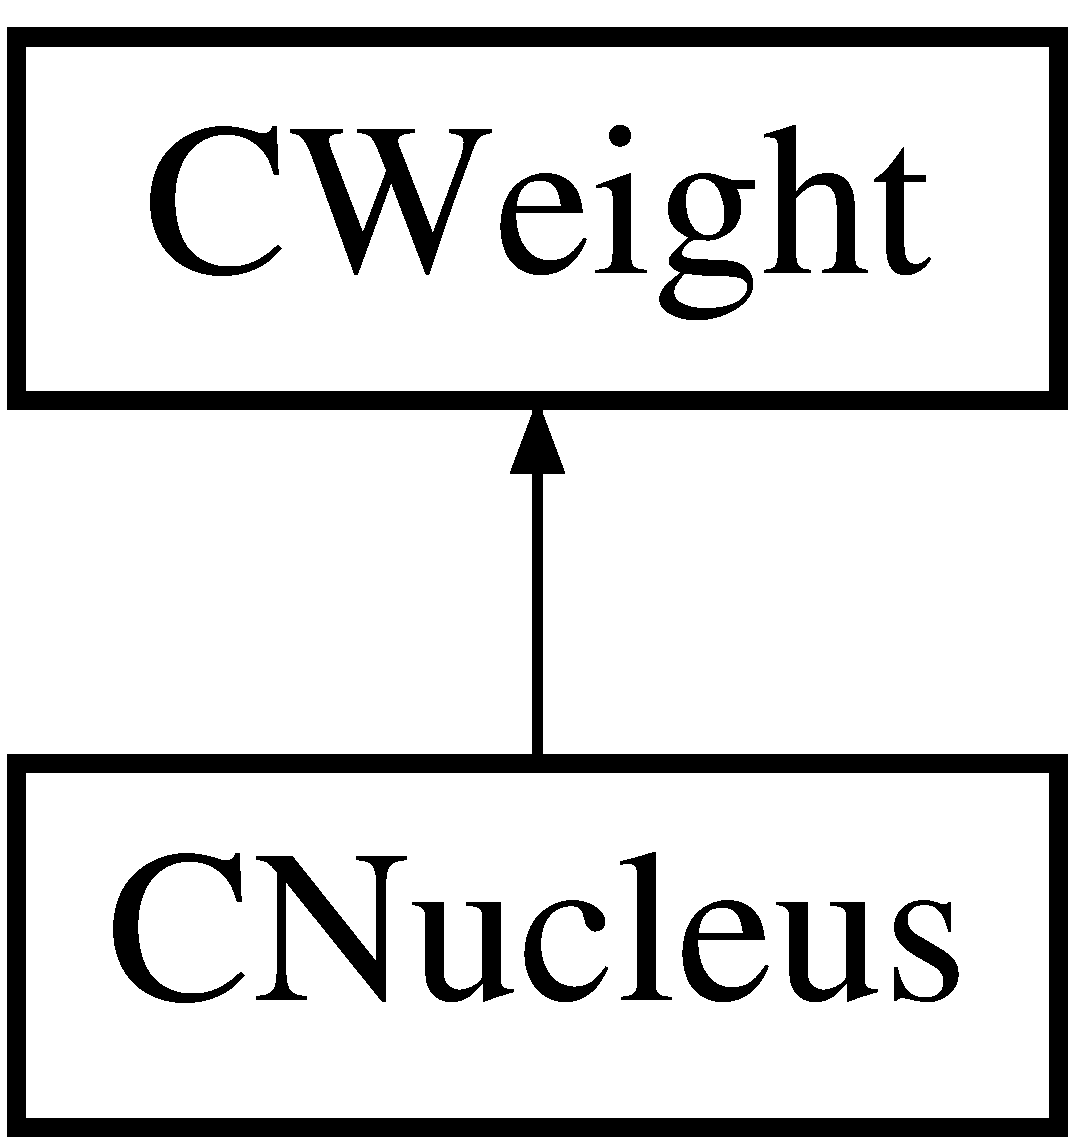
\includegraphics[height=2cm]{classCWeight}
\end{center}
\end{figure}
\subsection*{Public Member Functions}
\begin{CompactItemize}
\item 
int \bf{choose\-Channel} (float Glight, float Gimf, float Gfission, float Ggamma, float xran)
\item 
void \bf{set\-Weight\-IMF} ()
\item 
float \bf{get\-Weight\-Factor} ()
\end{CompactItemize}
\subsection*{Protected Member Functions}
\begin{CompactItemize}
\item 
void \bf{find\-Factor} (float Glight, float Gimf, float Gfission, float Ggamma)
\end{CompactItemize}
\subsection*{Protected Attributes}
\begin{CompactItemize}
\item 
float \bf{fact}\label{classCWeight_3b15fe630120a57701652a270d40ebd6}

\begin{CompactList}\small\item\em weighting factor \item\end{CompactList}\item 
int \bf{i\-Weight}\label{classCWeight_6027a33246e698010f4fd7ef204c906b}

\begin{CompactList}\small\item\em ==0, no weighting \item\end{CompactList}\item 
float \bf{running\-Weight}\label{classCWeight_56291a1271f65a303a587de31b5705bb}

\begin{CompactList}\small\item\em running weight of event \item\end{CompactList}\end{CompactItemize}


\subsection{Detailed Description}
weighted Monte Carlo 

!

Class \doxyref{CWeight}{p.}{classCWeight} is a base class that deals with a weighted Monte Carlo scheme. It is used to enhance the probabilty of IMF emission. To compensate for this, each event is given a weight. This weight should be used when histogramming events. 



\subsection{Member Function Documentation}
\index{CWeight@{CWeight}!chooseChannel@{chooseChannel}}
\index{chooseChannel@{chooseChannel}!CWeight@{CWeight}}
\subsubsection{\setlength{\rightskip}{0pt plus 5cm}int CWeight::choose\-Channel (float {\em gamma\-Light}, float {\em gamma\-Imf}, float {\em gamma\-Fission}, float {\em gamma\-Gamma}, float {\em xran})}\label{classCWeight_78edd0575c7fc5482866795d3052f5df}


Chooses the decay channel given the decay widths. If IMF weighting is truned on, then IMF emission is enhanced and a running weight is calculated. \begin{Desc}
\item[Parameters:]
\begin{description}
\item[{\em gamma\-Light}]decay width for light-particle evaporation (Me\-V) \item[{\em gamma\-Imf}]decay width for IMF emission (Me\-V) \item[{\em gamma\-Fission}]Fission decay width (Me\-V) \item[{\em gamma\-Gamma}]Gamma-ray decay width \item[{\em xran}]Random number \end{description}
\end{Desc}
\index{CWeight@{CWeight}!findFactor@{findFactor}}
\index{findFactor@{findFactor}!CWeight@{CWeight}}
\subsubsection{\setlength{\rightskip}{0pt plus 5cm}void CWeight::find\-Factor (float {\em gamma\-Light}, float {\em gamma\-Imf}, float {\em gamma\-Fission}, float {\em gamma\-Gamma})\hspace{0.3cm}{\tt  [protected]}}\label{classCWeight_38cdf3b427d8a20178e8a9d8dfb63fb5}


Determines the degree of weighting for enhance IMF emission \begin{Desc}
\item[Parameters:]
\begin{description}
\item[{\em gamma\-Light}]decay width for light-particle evaporation (Me\-V) \item[{\em gamma\-Imf}]decay width for IMF emission (Me\-V) \item[{\em gamma\-Fission}]Fission decay width (Me\-V) \item[{\em gamma\-Gamma}]Gamma-ray decay width \end{description}
\end{Desc}
\index{CWeight@{CWeight}!getWeightFactor@{getWeightFactor}}
\index{getWeightFactor@{getWeightFactor}!CWeight@{CWeight}}
\subsubsection{\setlength{\rightskip}{0pt plus 5cm}float CWeight::get\-Weight\-Factor ()}\label{classCWeight_3c7b2f6250ecf2eedecee982a72a7b7a}


When IMF weighting is turn on, this routine returns the weighting factor which should be used to increment all histograms. If weighting is turned off, then unity is returned \index{CWeight@{CWeight}!setWeightIMF@{setWeightIMF}}
\index{setWeightIMF@{setWeightIMF}!CWeight@{CWeight}}
\subsubsection{\setlength{\rightskip}{0pt plus 5cm}void CWeight::set\-Weight\-IMF ()}\label{classCWeight_e1262ad2c5320a2127a0fff5a8438771}


turns on IMF weighting, i.e. emhanced IMF emissions 

The documentation for this class was generated from the following files:\begin{CompactItemize}
\item 
CWeight.h\item 
Weight.cpp\end{CompactItemize}

\section{CYrast Class Reference}
\label{classCYrast}\index{CYrast@{CYrast}}
fission barriers, rotational energies, etc  


{\tt \#include $<$CYrast.h$>$}

\subsection*{Public Member Functions}
\begin{CompactItemize}
\item 
float \bf{get\-Yrast} (int, int, float)
\item 
float \bf{get\-Yrast\-Model} (int, int, float)
\item 
float \bf{get\-Yrast\-RLDM} (int, int, float)
\item 
float \bf{get\-Yrast\-Sierk} (float)
\item 
float \bf{get\-Jmax\-Sierk} (int, int)
\item 
float \bf{get\-Barrier\-Fission\-Sierk} (float)
\item 
float \bf{get\-Symmetric\-Saddle\-Energy} (int, int, float)
\item 
float \bf{get\-Barrier\-Fission\-RLDM} (int, int, float)
\item 
float \bf{get\-Bs\-Sierk} (float)
\item 
void \bf{prepare\-Asy\-Barrier} (int, int, float)
\item 
void \bf{print\-Asy\-Barrier} ()
\item 
float \bf{get\-Saddle\-Point\-Energy} (int, int)
\item 
float \bf{get\-Saddle\-Point\-Energy} (float)
\item 
float \bf{get\-Moment\-Of\-Inertia\-Sierk} (float)
\item 
float \bf{Wigner\-Energy} (int \bf{i\-Z}, int \bf{i\-A})
\end{CompactItemize}
\subsection*{Static Public Member Functions}
\begin{CompactItemize}
\item 
static \bf{CYrast} $\ast$ \bf{instance} ()\label{classCYrast_f8bd90dce7a0e85b472f1e0620ad7de4}

\begin{CompactList}\small\item\em instance member to make this class a singleton \item\end{CompactList}\item 
static void \bf{force\-Sierk} (bool=1)
\item 
static void \bf{print\-Parameters} ()
\end{CompactItemize}
\subsection*{Public Attributes}
\begin{CompactItemize}
\item 
double \bf{Jmax}\label{classCYrast_f519cefa302fd96cc59f1e199647b7a1}

\begin{CompactList}\small\item\em max spin where the fission barrier exists \item\end{CompactList}\item 
float \bf{mom\-Inertia\-Min}\label{classCYrast_ceeac2c16a69d9b375730d71d21087f9}

\begin{CompactList}\small\item\em minimum saddle-point moment of inertia \item\end{CompactList}\item 
float \bf{mom\-Inertia\-Mid}\label{classCYrast_dbc30c7f47cac4f12af9a11bd1e43925}

\begin{CompactList}\small\item\em intermediate saddle-point moment of inertia \item\end{CompactList}\item 
float \bf{mom\-Inertia\-Max}\label{classCYrast_49fdeeb99a27ac65b453f922b70d995e}

\begin{CompactList}\small\item\em maximum saddle-point moment of inertia \item\end{CompactList}\end{CompactItemize}
\subsection*{Private Member Functions}
\begin{CompactItemize}
\item 
\bf{CYrast} ()
\item 
void \bf{lpoly} (double, int, double $\ast$)
\item 
float \bf{cubic} (float, float, float, float, float, float)
\end{CompactItemize}
\subsection*{Private Attributes}
\begin{CompactItemize}
\item 
double \bf{A}\label{classCYrast_b5bd91cce2e946b7c85556e079e5d660}

\begin{CompactList}\small\item\em mass number \item\end{CompactList}\item 
double \bf{Z}\label{classCYrast_4636ed540d5223b745cf1182e25589fa}

\begin{CompactList}\small\item\em proton number \item\end{CompactList}\item 
double \bf{zz}\label{classCYrast_de32dc096261e4c87d077bba15a104b2}

\begin{CompactList}\small\item\em used in Sierk functions \item\end{CompactList}\item 
double \bf{amin}\label{classCYrast_28b989d08b3c8efe5173d5acc7c8ae64}

\begin{CompactList}\small\item\em lower limits of application of Sierk routine \item\end{CompactList}\item 
double \bf{amax}\label{classCYrast_d155cae6125420fb66b6a1e57bb64e76}

\begin{CompactList}\small\item\em upper limits of application of Sierk routine \item\end{CompactList}\item 
double \bf{pa} [7]\label{classCYrast_1f61886b08482ea983bbb552897e35d2}

\begin{CompactList}\small\item\em used in Sierk routines \item\end{CompactList}\item 
double \bf{pz} [7]\label{classCYrast_a0e96b3bf3446d6a291bb023c01259db}

\begin{CompactList}\small\item\em used in Sierk routines \item\end{CompactList}\item 
float \bf{c} [6][8][2][11][2]\label{classCYrast_09f29bfb774077e0d7996ccb8d7f0884}

\begin{CompactList}\small\item\em coeff for sadfits \item\end{CompactList}\item 
int \bf{Narray}\label{classCYrast_97e5bc8a53cebc53bd41f50004139a9a}

\begin{CompactList}\small\item\em number of elements in array of asymmetric barriers \item\end{CompactList}\item 
float \bf{sad\-Array} [300]\label{classCYrast_b9a730e3c26607de2675f58b9c587d6b}

\begin{CompactList}\small\item\em array stores the conditional saddle energies \item\end{CompactList}\item 
float \bf{sad\-Array\-ZA} [300]\label{classCYrast_52b607a9aaf5ce26feee1ad8fcd4a24f}

\begin{CompactList}\small\item\em array stores saddle energies after correction \item\end{CompactList}\item 
\bf{CMass} $\ast$ \bf{mass}\label{classCYrast_7228575eb0933e72dcdf6386a51f1802}

\begin{CompactList}\small\item\em class for mass defects \item\end{CompactList}\item 
int \bf{i\-Z}\label{classCYrast_748e9f8b7ea2129711755345dbbe8b1f}

\begin{CompactList}\small\item\em proton number \item\end{CompactList}\item 
int \bf{i\-A}\label{classCYrast_37e83874a21b3dea25708215649815fb}

\begin{CompactList}\small\item\em mass number \item\end{CompactList}\item 
float \bf{f\-J}\label{classCYrast_d2f214b7d12672a5f92561de9d0fdf57}

\begin{CompactList}\small\item\em spin \item\end{CompactList}\end{CompactItemize}
\subsection*{Static Private Attributes}
\begin{CompactItemize}
\item 
static \bf{CYrast} $\ast$ \bf{f\-Instance} = 0\label{classCYrast_e06b12d4f459e11a7b7fe2c310d8fe7c}

\begin{CompactList}\small\item\em instance member to make this class a singleton \item\end{CompactList}\item 
static double const \bf{pi} = acos(-1.)\label{classCYrast_d4868c17ce6a605e9501bd0761a776c0}

\begin{CompactList}\small\item\em 3.14159 \item\end{CompactList}\item 
static float const \bf{x1h} [11][6]
\begin{CompactList}\small\item\em number for RLDM \item\end{CompactList}\item 
static float const \bf{x2h} [11][6]
\begin{CompactList}\small\item\em numbers for RLDM \item\end{CompactList}\item 
static float const \bf{x3h} [20][10]
\begin{CompactList}\small\item\em number for RLDM \item\end{CompactList}\item 
static float const \bf{x1b} [11][6]
\begin{CompactList}\small\item\em numbers for RLDM \item\end{CompactList}\item 
static float const \bf{x2b} [11][6]
\begin{CompactList}\small\item\em numbers for RLDM \item\end{CompactList}\item 
static float const \bf{x3b} [20][10]
\begin{CompactList}\small\item\em numbers for RLDM \item\end{CompactList}\item 
static double const \bf{emncof} [4][5]
\begin{CompactList}\small\item\em used in Sierk functions \item\end{CompactList}\item 
static double const \bf{elmcof} [4][5]
\begin{CompactList}\small\item\em used in Sierk functions \item\end{CompactList}\item 
static double const \bf{emxcof} [5][7]
\begin{CompactList}\small\item\em used in Sierk functions \item\end{CompactList}\item 
static double const \bf{elzcof} [7][7]
\begin{CompactList}\small\item\em used in Sierk functions \item\end{CompactList}\item 
static double const \bf{egscof} [5][7][5]\label{classCYrast_799a76146e8fbbf27abbb7b5f7894b6d}

\begin{CompactList}\small\item\em used in Sierk functions \item\end{CompactList}\item 
static double const \bf{aizroc} [5][6]
\begin{CompactList}\small\item\em used in Sierk functions \item\end{CompactList}\item 
static double const \bf{ai70c} [5][6]
\begin{CompactList}\small\item\em used in Sierk functions \item\end{CompactList}\item 
static double const \bf{ai95c} [5][6]
\begin{CompactList}\small\item\em used in Sierk functions \item\end{CompactList}\item 
static double const \bf{aimaxc} [5][6]
\begin{CompactList}\small\item\em used in Sierk functions \item\end{CompactList}\item 
static double const \bf{ai952c} [5][6]
\begin{CompactList}\small\item\em used in Sierk functions \item\end{CompactList}\item 
static double const \bf{aimax2c} [5][6]
\begin{CompactList}\small\item\em used in Sierk functions \item\end{CompactList}\item 
static double const \bf{aimax3c} [4][4]
\begin{CompactList}\small\item\em used in Sierk functions \item\end{CompactList}\item 
static double const \bf{aimax4c} [4][4]
\begin{CompactList}\small\item\em used in Sierk functions \item\end{CompactList}\item 
static double const \bf{bizroc} [4][6]
\begin{CompactList}\small\item\em used in Sierk functions \item\end{CompactList}\item 
static double const \bf{bi70c} [4][6]
\begin{CompactList}\small\item\em used in Sierk functions \item\end{CompactList}\item 
static double const \bf{bi95c} [4][6]
\begin{CompactList}\small\item\em used in Sierk functions \item\end{CompactList}\item 
static double const \bf{bimaxc} [4][6]
\begin{CompactList}\small\item\em used in Sierk functions \item\end{CompactList}\item 
static double const \bf{b} [8][5][5]\label{classCYrast_1fbcff30f8e42d75edf43a66856cb2f1}

\begin{CompactList}\small\item\em used in Sierk functions \item\end{CompactList}\item 
static bool \bf{first} = 1\label{classCYrast_bfb8faabafae56d6e24463802b69653c}

\begin{CompactList}\small\item\em only write out barrier warning once \item\end{CompactList}\item 
static float const \bf{hbarc} = 197.32858\label{classCYrast_360ded0bfb6c3e0790f13938a07b5934}

\begin{CompactList}\small\item\em used for asymmetric barriers \item\end{CompactList}\item 
static float const \bf{alfinv} = 137.035982\label{classCYrast_63e8a1078a711dcf1776154bcc19ad0a}

\begin{CompactList}\small\item\em used for asymmetric barriers \item\end{CompactList}\item 
static float const \bf{srznw} = 1.16\label{classCYrast_405e9b958ae2c3a1a1b0404bb287c8ca}

\begin{CompactList}\small\item\em used for asymmetric barriers \item\end{CompactList}\item 
static float const \bf{aknw} = 2.3\label{classCYrast_0360a5e0d518c01e6c83c8cee68e6246}

\begin{CompactList}\small\item\em used for asymmetric barriers \item\end{CompactList}\item 
static float const \bf{bb} = 0.99\label{classCYrast_12d6e2131be8b706131c5131d393cdec}

\begin{CompactList}\small\item\em used for asymmetric barriers \item\end{CompactList}\item 
static float const \bf{um} = 931.5016\label{classCYrast_1893cc9dbe12d802fbfa46b9ca410132}

\begin{CompactList}\small\item\em used for asymmetric barriers \item\end{CompactList}\item 
static float const \bf{elm} = 0.51104\label{classCYrast_dd8fd2d61f6f12774b0f45219a96bd9c}

\begin{CompactList}\small\item\em used for asymmetric barriers \item\end{CompactList}\item 
static float const \bf{spdlt} = 2.99792458e23\label{classCYrast_ef0c5b00001a0e5ac3595e29090666a7}

\begin{CompactList}\small\item\em used for asymmetric barriers \item\end{CompactList}\item 
static float const \bf{asnw} = 21.13\label{classCYrast_d95be4ebfdd77b7a5cc099949c4c118e}

\begin{CompactList}\small\item\em used for asymmetric barriers \item\end{CompactList}\item 
static float const \bf{kx} [8]
\begin{CompactList}\small\item\em used for asymmetric barriers \item\end{CompactList}\item 
static float const \bf{ky} [6] = \{0.0,0.02,0.05,0.10,0.15,0.20\}\label{classCYrast_e3ed9fa393f06f9b740a6dc4fb15084c}

\begin{CompactList}\small\item\em used for asymmetric barriers \item\end{CompactList}\item 
static float const \bf{ka} [11] = \{0.0,.1,.2,.3,.4,.5,.6,.7,.8,.9,1.\}\label{classCYrast_1fe225848928940480cc32aeae0eeeac}

\begin{CompactList}\small\item\em used for asymmetric barriers \item\end{CompactList}\item 
static float const \bf{r0} = 1.225\label{classCYrast_1624d25a5700c629cc77c7d6132bbf83}

\begin{CompactList}\small\item\em radius parameter \item\end{CompactList}\item 
static float const \bf{sep} = 2.\label{classCYrast_0d79dbacd24d2c52cdd14afb596dc4cb}

\begin{CompactList}\small\item\em separation id fm between fragments \item\end{CompactList}\item 
static bool \bf{b\-Force\-Sierk} = 0\label{classCYrast_a3121d15a3b423542d992a227143c299}

\begin{CompactList}\small\item\em separation id fm between fragments \item\end{CompactList}\item 
static double \bf{add\-Bar} = 0.\label{classCYrast_6ec4fd97f4faf45d2a751035c273c000}

\begin{CompactList}\small\item\em extrapolated Sierk barrier increase by this amount \item\end{CompactList}\item 
static float const \bf{delta\-J} = 3.\label{classCYrast_827b6f607143264fbe1a3201ad0a2a79}

\begin{CompactList}\small\item\em used to extend sierk barrier to higher J \item\end{CompactList}\item 
static float const \bf{k\-Rotate} = 41.563\label{classCYrast_0420fc3a7b42a85e2959ac5296ab5ce2}

\begin{CompactList}\small\item\em constant for rotional energy \item\end{CompactList}\end{CompactItemize}


\subsection{Detailed Description}
fission barriers, rotational energies, etc 

!

Class to return barriers and rotational energies. It is constructed from bits of code such as Arnie Sierk Barfit - which gives his Finite-range fission barrier, rotational energies, moments of inertia, surface areas. Also I have used code from the RLDM model. In addition I enclude a interpolation of conditional fission barriers, using barriers calculated by Sierk 



\subsection{Constructor \& Destructor Documentation}
\index{CYrast@{CYrast}!CYrast@{CYrast}}
\index{CYrast@{CYrast}!CYrast@{CYrast}}
\subsubsection{\setlength{\rightskip}{0pt plus 5cm}CYrast::CYrast ()\hspace{0.3cm}{\tt  [private]}}\label{classCYrast_c921da56f10301d8a1fc46c57c0fc73f}


Constructor 

\subsection{Member Function Documentation}
\index{CYrast@{CYrast}!cubic@{cubic}}
\index{cubic@{cubic}!CYrast@{CYrast}}
\subsubsection{\setlength{\rightskip}{0pt plus 5cm}float CYrast::cubic (float {\em a}, float {\em b}, float {\em c}, float {\em d}, float {\em e}, float {\em f})\hspace{0.3cm}{\tt  [private]}}\label{classCYrast_91dccad458ce86b53d4c8581138b59fd}


Cubic polynomial used in 2D cubic spline interpolation \index{CYrast@{CYrast}!forceSierk@{forceSierk}}
\index{forceSierk@{forceSierk}!CYrast@{CYrast}}
\subsubsection{\setlength{\rightskip}{0pt plus 5cm}void CYrast::force\-Sierk (bool {\em b} = {\tt 1})\hspace{0.3cm}{\tt  [static]}}\label{classCYrast_faa29df45ab999a03a954c5c3fcceafc}


Forces the use of Sierk yrast energies. As Default GEMINI++ uses a modified YRAST line for light nuclei so as to get the shape of the alpha-particle evaporation spectra correct. \index{CYrast@{CYrast}!getBarrierFissionRLDM@{getBarrierFissionRLDM}}
\index{getBarrierFissionRLDM@{getBarrierFissionRLDM}!CYrast@{CYrast}}
\subsubsection{\setlength{\rightskip}{0pt plus 5cm}float CYrast::get\-Barrier\-Fission\-RLDM (int {\em i\-Z}, int {\em i\-A}, float {\em f\-J})}\label{classCYrast_5a1b61afbb39ecf59a4d64fbe8a90455}


Returns the fission barrier in Me\-V from the Rotating Liquid Drop Model. \begin{Desc}
\item[Parameters:]
\begin{description}
\item[{\em i\-Z}]is the proton number. \item[{\em i\-A}]is the mass number \item[{\em f\-J}]is the angular momentum \end{description}
\end{Desc}
\index{CYrast@{CYrast}!getBarrierFissionSierk@{getBarrierFissionSierk}}
\index{getBarrierFissionSierk@{getBarrierFissionSierk}!CYrast@{CYrast}}
\subsubsection{\setlength{\rightskip}{0pt plus 5cm}float CYrast::get\-Barrier\-Fission\-Sierk (float {\em J})}\label{classCYrast_f02af67414db1d93a36feac1a756828a}


Returns the fission barrier from the model of Sierk. Units are in Me\-V. The function \doxyref{get\-Jmax\-Sierk()}{p.}{classCYrast_6cbaefdb9dd6c01be0b8efd4f7e5bc6c} must be called beforehand \begin{Desc}
\item[Parameters:]
\begin{description}
\item[{\em J}]is the angular momentum in hbar \end{description}
\end{Desc}
\index{CYrast@{CYrast}!getBsSierk@{getBsSierk}}
\index{getBsSierk@{getBsSierk}!CYrast@{CYrast}}
\subsubsection{\setlength{\rightskip}{0pt plus 5cm}float CYrast::get\-Bs\-Sierk (float {\em J})}\label{classCYrast_be3a2ab5f3822f5dbe4230668be8d45d}


Returns the relative surface area of the saddle-point shape from the model of Sierk. The surface is relative to the value for a spherical nucleus \begin{Desc}
\item[Parameters:]
\begin{description}
\item[{\em J}]is the angular momentum \end{description}
\end{Desc}
\index{CYrast@{CYrast}!getJmaxSierk@{getJmaxSierk}}
\index{getJmaxSierk@{getJmaxSierk}!CYrast@{CYrast}}
\subsubsection{\setlength{\rightskip}{0pt plus 5cm}float CYrast::get\-Jmax\-Sierk (int {\em i\-Z}, int {\em i\-A})}\label{classCYrast_6cbaefdb9dd6c01be0b8efd4f7e5bc6c}


Returns the Maximum angular momentum where the nucleus is stable against fission in the model of Sierk. ie. above this value the barrier vanishes. Units are in hbar. \begin{Desc}
\item[Parameters:]
\begin{description}
\item[{\em i\-Z}]is proton number \item[{\em i\-A}]is the mass number \end{description}
\end{Desc}
\index{CYrast@{CYrast}!getMomentOfInertiaSierk@{getMomentOfInertiaSierk}}
\index{getMomentOfInertiaSierk@{getMomentOfInertiaSierk}!CYrast@{CYrast}}
\subsubsection{\setlength{\rightskip}{0pt plus 5cm}float CYrast::get\-Moment\-Of\-Inertia\-Sierk (float {\em J})}\label{classCYrast_b6f720d2b14822a77ecb1cd0de030ea2}


Calculates the three principle moments of inertia associated with the saddle-point configuration in the model of Sierk.The function get\-Jmax\-Sierk must be called beforehand. \begin{Desc}
\item[Parameters:]
\begin{description}
\item[{\em J}]is the angular momentum \end{description}
\end{Desc}
\index{CYrast@{CYrast}!getSaddlePointEnergy@{getSaddlePointEnergy}}
\index{getSaddlePointEnergy@{getSaddlePointEnergy}!CYrast@{CYrast}}
\subsubsection{\setlength{\rightskip}{0pt plus 5cm}float CYrast::get\-Saddle\-Point\-Energy (float {\em A1})}\label{classCYrast_39424851fed9d58619f4f0df060c1c5e}


Returns the conditioanl saddle-point energy when both nascient fragments have the same Z/A as the parent nucleus /param A1 is the mass number of one of the nascient fragments \index{CYrast@{CYrast}!getSaddlePointEnergy@{getSaddlePointEnergy}}
\index{getSaddlePointEnergy@{getSaddlePointEnergy}!CYrast@{CYrast}}
\subsubsection{\setlength{\rightskip}{0pt plus 5cm}float CYrast::get\-Saddle\-Point\-Energy (int {\em i\-Z1}, int {\em i\-A1})}\label{classCYrast_8d4ac8b8baa0004c4f964e5a9e430418}


Returns the constrained saddle-point energy for channel where one of the fragmenst is i\-Z1,i\-A1 \begin{Desc}
\item[Parameters:]
\begin{description}
\item[{\em i\-Z1}]is the proton number \item[{\em i\-A1}]is the mass number \end{description}
\end{Desc}
\index{CYrast@{CYrast}!getSymmetricSaddleEnergy@{getSymmetricSaddleEnergy}}
\index{getSymmetricSaddleEnergy@{getSymmetricSaddleEnergy}!CYrast@{CYrast}}
\subsubsection{\setlength{\rightskip}{0pt plus 5cm}float CYrast::get\-Symmetric\-Saddle\-Energy (int {\em i\-Z}, int {\em i\-A}, float {\em f\-J})}\label{classCYrast_d0a0a2d6ac4db8dc618e4e880f8ccd30}


Returns the saddle-point energy for symmetric fission in units of Me\-V \begin{Desc}
\item[Parameters:]
\begin{description}
\item[{\em i\-Z}]is the proton number \item[{\em i\-A}]is the mass number \item[{\em f\-J}]is the angular momentum \end{description}
\end{Desc}
\index{CYrast@{CYrast}!getYrast@{getYrast}}
\index{getYrast@{getYrast}!CYrast@{CYrast}}
\subsubsection{\setlength{\rightskip}{0pt plus 5cm}float CYrast::get\-Yrast (int {\em i\-Z}, int {\em i\-A}, float {\em f\-J})}\label{classCYrast_3d52c1b86cb26e776b5df02118316ad9}


General call to get Yrast energy, includes a fix for light nuclear so that the Yrast line does not become to steep. At a spin JChange, the Yrast line continues with a constant slope.

\begin{Desc}
\item[Parameters:]
\begin{description}
\item[{\em i\-Z}]is the proton number \item[{\em i\-A}]is the mass number \item[{\em f\-J}]is the angular momentum \end{description}
\end{Desc}
\index{CYrast@{CYrast}!getYrastModel@{getYrastModel}}
\index{getYrastModel@{getYrastModel}!CYrast@{CYrast}}
\subsubsection{\setlength{\rightskip}{0pt plus 5cm}float CYrast::get\-Yrast\-Model (int {\em i\-Z}, int {\em i\-A}, float {\em f\-J})}\label{classCYrast_619515cfa0f43558880e335dd8bebb64}


General call to get Yrast energy according to Nuclear models This handles probems if i\-A is too small or the angular momentum is too large in extrapolating the Yrast line. \begin{Desc}
\item[Parameters:]
\begin{description}
\item[{\em i\-Z}]is the proton number \item[{\em i\-A}]is the mass number \item[{\em f\-J}]is the angular momentum \end{description}
\end{Desc}
\index{CYrast@{CYrast}!getYrastRLDM@{getYrastRLDM}}
\index{getYrastRLDM@{getYrastRLDM}!CYrast@{CYrast}}
\subsubsection{\setlength{\rightskip}{0pt plus 5cm}float CYrast::get\-Yrast\-RLDM (int {\em i\-Z}, int {\em i\-A}, float {\em f\-L})}\label{classCYrast_289214476f9d672676dd81cfd4b1f966}


Returns the yrast energy in Me\-V from the Rotating Liquid Drop Model \begin{Desc}
\item[Parameters:]
\begin{description}
\item[{\em i\-Z}]is the proton number \item[{\em i\-A}]is the mass number \item[{\em f\-L}]is the angular momentum in hbar \end{description}
\end{Desc}
\index{CYrast@{CYrast}!getYrastSierk@{getYrastSierk}}
\index{getYrastSierk@{getYrastSierk}!CYrast@{CYrast}}
\subsubsection{\setlength{\rightskip}{0pt plus 5cm}float CYrast::get\-Yrast\-Sierk (float {\em J})}\label{classCYrast_9c54905c80cca507c85c1f092e027b01}


Returns the yrast energy is trhe model of Sierk. Units are in Me\-V. The function get\-Jmaz\-Sierk must be called beforehand. \begin{Desc}
\item[Parameters:]
\begin{description}
\item[{\em J}]is the angular momentum \end{description}
\end{Desc}
\index{CYrast@{CYrast}!lpoly@{lpoly}}
\index{lpoly@{lpoly}!CYrast@{CYrast}}
\subsubsection{\setlength{\rightskip}{0pt plus 5cm}void CYrast::lpoly (double {\em x}, int {\em n}, double $\ast$ {\em pl})\hspace{0.3cm}{\tt  [private]}}\label{classCYrast_d58e02c0cbefdd045f3fc7624cf8c75f}


calculates a array of Legendre Polynomials \begin{Desc}
\item[Parameters:]
\begin{description}
\item[{\em x}]is the independent variable \item[{\em n}]is the maximum order of the array \item[{\em pl}]is the pointer to the array \end{description}
\end{Desc}
\index{CYrast@{CYrast}!prepareAsyBarrier@{prepareAsyBarrier}}
\index{prepareAsyBarrier@{prepareAsyBarrier}!CYrast@{CYrast}}
\subsubsection{\setlength{\rightskip}{0pt plus 5cm}void CYrast::prepare\-Asy\-Barrier (int {\em i\-Z0}, int {\em i\-A0}, float {\em f\-J0})}\label{classCYrast_576979fab8d2b2ecf26d0274f4254171}


Prepares for the calculation of conditional saddle-point energies in Me\-V \begin{Desc}
\item[Parameters:]
\begin{description}
\item[{\em i\-Z0}]is the proton number \item[{\em i\-A0}]is the mass number \item[{\em f\-J0}]is the angular momentum in hbar \end{description}
\end{Desc}
\index{CYrast@{CYrast}!printAsyBarrier@{printAsyBarrier}}
\index{printAsyBarrier@{printAsyBarrier}!CYrast@{CYrast}}
\subsubsection{\setlength{\rightskip}{0pt plus 5cm}void CYrast::print\-Asy\-Barrier ()}\label{classCYrast_72432ca895255edf1f5fdbaa8333d54f}


Prints out the array of conditional barriers \index{CYrast@{CYrast}!printParameters@{printParameters}}
\index{printParameters@{printParameters}!CYrast@{CYrast}}
\subsubsection{\setlength{\rightskip}{0pt plus 5cm}void CYrast::print\-Parameters ()\hspace{0.3cm}{\tt  [static]}}\label{classCYrast_e7c7e015ce294a114d94523bb3888a34}


Prints out the parameters used in the Yrast class \index{CYrast@{CYrast}!WignerEnergy@{WignerEnergy}}
\index{WignerEnergy@{WignerEnergy}!CYrast@{CYrast}}
\subsubsection{\setlength{\rightskip}{0pt plus 5cm}float CYrast::Wigner\-Energy (int {\em i\-Z}, int {\em i\-A})}\label{classCYrast_2e6ad60aaba3564566f0433326a33d2c}


calculates the Wigner energy in the mass formula used by Sierk \begin{Desc}
\item[Parameters:]
\begin{description}
\item[{\em i\-Z}]is the proton number \item[{\em i\-A}]is the mass number \end{description}
\end{Desc}


\subsection{Member Data Documentation}
\index{CYrast@{CYrast}!ai70c@{ai70c}}
\index{ai70c@{ai70c}!CYrast@{CYrast}}
\subsubsection{\setlength{\rightskip}{0pt plus 5cm}double const \bf{CYrast::ai70c}\hspace{0.3cm}{\tt  [static, private]}}\label{classCYrast_c09db25ae06ba1174a6b92e06acd9f80}


\textbf{Initial value:}

\begin{Code}\begin{verbatim}{
{ 3.11420101e4,-7.54335155e4, 7.74456473e4,-4.79993065e4,
 2.23439118e4,-4.81961155e3},
{-7.24025043e4, 1.72276697e5,-1.72027101e5, 1.03891065e5,
-4.83180786e4, 1.08040504e4},
{ 7.14932917e4,-1.72792523e5, 1.75814382e5,-1.07245918e5,
 4.86163223e4,-1.10623761e4},
{-2.87206866e4, 6.76667976e4,-6.50167483e4, 3.67161268e4,
-1.74755753e4, 4.67495427e3},
{1.67914908e4,-3.97304542e4, 3.81446552e4,-2.04628156e4,
   7.20091899e3,-1.49978283e3}}
\end{verbatim}\end{Code}
used in Sierk functions 

\index{CYrast@{CYrast}!ai952c@{ai952c}}
\index{ai952c@{ai952c}!CYrast@{CYrast}}
\subsubsection{\setlength{\rightskip}{0pt plus 5cm}double const \bf{CYrast::ai952c}\hspace{0.3cm}{\tt  [static, private]}}\label{classCYrast_93ae1f8c032b456157de5c1279ced712}


\textbf{Initial value:}

\begin{Code}\begin{verbatim}{
  {-7.37473153e5, 1.73682827e6,-1.75850175e6, 1.11320647e6, 
   -4.41842735e5, 9.02463457e4},
  { 1.49541980e6,-3.53222507e6, 3.59762757e6,-2.29652257e6,
    9.21077757e5,-1.90079527e5},
  {-1.80243593e6, 4.24319661e6,-4.29072662e6, 2.71416936e6,
   -1.07624953e6, 2.20863711e5},
  { 8.86920591e5,-2.09589683e6,2.13507675e6,-1.36546686e6,
    5.48868536e5,-1.14532906e5},
  {-4.62131503e5, 1.08555722e6,-1.09187524e6, 6.87308217e5,
   -2.70986162e5, 5.61637883e4}}
\end{verbatim}\end{Code}
used in Sierk functions 

\index{CYrast@{CYrast}!ai95c@{ai95c}}
\index{ai95c@{ai95c}!CYrast@{CYrast}}
\subsubsection{\setlength{\rightskip}{0pt plus 5cm}double const \bf{CYrast::ai95c}\hspace{0.3cm}{\tt  [static, private]}}\label{classCYrast_2381c41d4de825156d5828349ca301ba}


\textbf{Initial value:}

\begin{Code}\begin{verbatim}{
{-6.17201449e5, 1.45561724e6,-1.47514522e6, 9.37798508e5,
-3.74435017e5, 7.81254880e4},
{ 1.24304280e6,-2.94179116e6, 3.00170753e6,-1.92737183e6,
 7.79238772e5,-1.64803784e5},
{-1.49648799e6, 3.52658199e6,-3.56784327e6, 2.26413602e6,
-9.02243251e5, 1.88619658e5},
{ 7.27293223e5,-1.72140677e6,1.75634889e6,-1.12885888e6,
 4.57150814e5,-9.74833991e4},
{-3.75965723e5, 8.83032946e5,-8.87134867e5, 5.58350462e5,
 -2.20433857e5, 4.62178756e4}}
\end{verbatim}\end{Code}
used in Sierk functions 

\index{CYrast@{CYrast}!aimax2c@{aimax2c}}
\index{aimax2c@{aimax2c}!CYrast@{CYrast}}
\subsubsection{\setlength{\rightskip}{0pt plus 5cm}double const \bf{CYrast::aimax2c}\hspace{0.3cm}{\tt  [static, private]}}\label{classCYrast_3bc0006f8c3bf7fc99e0e5b709ebdd57}


\textbf{Initial value:}

\begin{Code}\begin{verbatim}{
  {-1.16343311e6, 2.74470544e6,-2.77664273e6, 1.76933559e6,
   -7.02900226e5, 1.49345081e5},
  { 2.36929777e6,-5.60655122e6,5.70413177e6,-3.66528765e6,
    1.47006527e6,-3.15794626e5},
  {-2.82646077e6, 6.66086824e6,-6.72677653e6, 4.27484625e6,
   -1.69427298e6, 3.58429081e5},
  { 1.39112772e6,-3.29007553e6, 3.34544584e6,-2.14723142e6,
    8.61118401e5,-1.84500129e5},
  {-7.21329917e5, 1.69371794e6,-1.69979786e6, 1.07037781e6,
   -4.20662028e5, 8.80728361e4}}
\end{verbatim}\end{Code}
used in Sierk functions 

\index{CYrast@{CYrast}!aimax3c@{aimax3c}}
\index{aimax3c@{aimax3c}!CYrast@{CYrast}}
\subsubsection{\setlength{\rightskip}{0pt plus 5cm}double const \bf{CYrast::aimax3c}\hspace{0.3cm}{\tt  [static, private]}}\label{classCYrast_f2dee1bf2f45cdd156673843590eb948}


\textbf{Initial value:}

\begin{Code}\begin{verbatim}{
  {-2.88270282e3, 5.30111305e3,-3.07626751e3,6.56709396e2},
  {5.84303930e3,-1.07450449e4,6.24110631e3,-1.33480875e3},
  {-4.20629939e3,7.74058373e3,-4.50256063e3, 9.65788439e2},
  {1.23820134e3,-2.28228958e3, 1.33181316e3,-2.87363568e2}}
\end{verbatim}\end{Code}
used in Sierk functions 

\index{CYrast@{CYrast}!aimax4c@{aimax4c}}
\index{aimax4c@{aimax4c}!CYrast@{CYrast}}
\subsubsection{\setlength{\rightskip}{0pt plus 5cm}double const \bf{CYrast::aimax4c}\hspace{0.3cm}{\tt  [static, private]}}\label{classCYrast_92f739a4d8d2e46a0479e954f80d8728}


\textbf{Initial value:}

\begin{Code}\begin{verbatim}{
  {-3.34060345e3, 6.26384099e3,-3.77635848e3, 8.57180868e2},
  { 6.76377873e3,-1.26776571e4, 7.64206952e3,-1.73406840e3},
  {-4.74821371e3, 8.89857519e3,-5.36266252e3, 1.21614216e3},
  { 1.46369384e3,-2.74251101e3, 1.65205435e3,-3.74262365e2}}
\end{verbatim}\end{Code}
used in Sierk functions 

\index{CYrast@{CYrast}!aimaxc@{aimaxc}}
\index{aimaxc@{aimaxc}!CYrast@{CYrast}}
\subsubsection{\setlength{\rightskip}{0pt plus 5cm}double const \bf{CYrast::aimaxc}\hspace{0.3cm}{\tt  [static, private]}}\label{classCYrast_4aba17c77ac5fcad545afb57d8dc76ef}


\textbf{Initial value:}

\begin{Code}\begin{verbatim}{
  {-1.07989556e6, 2.54617598e6,-2.56762409e6, 1.62814115e6,
   -6.39575059e5, 1.34017942e5},
  { 2.17095357e6,-5.13081589e6, 5.19610055e6,-3.31651644e6,
    1.31229476e6,-2.77511450e5},
  {-2.66020302e6, 6.26593165e6,-6.31060776e6, 3.99082969e6, 
   -1.56447660e6, 3.25613262e5},
  { 1.29464191e6,-3.05746938e6, 3.09487138e6,-1.97160118e6,
    7.79696064e5,-1.63704652e5},
  {-7.13073644e5, 1.67482279e6,-1.67984330e6, 1.05446783e6,
   -4.10928559e5, 8.43774143e4}}
\end{verbatim}\end{Code}
used in Sierk functions 

\index{CYrast@{CYrast}!aizroc@{aizroc}}
\index{aizroc@{aizroc}!CYrast@{CYrast}}
\subsubsection{\setlength{\rightskip}{0pt plus 5cm}double const \bf{CYrast::aizroc}\hspace{0.3cm}{\tt  [static, private]}}\label{classCYrast_1b105b6fb7940bbe943b1d890a2fe508}


\textbf{Initial value:}

\begin{Code}\begin{verbatim}{
{ 2.34441624e4,-5.88023986e4, 6.37939552e4,-4.79085272e4, 
 2.27517867e4,-5.35372280e3},
{-4.19782127e4, 1.09187735e5,-1.24597673e5, 9.93997182e4,
-4.95141312e4, 1.19847414e4},
{ 4.18237803e4,-1.05557152e5, 1.16142947e5,-9.00443421e4,
 4.48976290e4,-1.10161792e4},
{-8.27172333e3, 2.49194412e4,-3.39090117e4, 3.33727886e4,
-1.98040399e4, 5.37766241e3},  
{ 5.79695749e2,-1.61762346e3, 2.14044262e3,-3.55379785e3,
    3.25502799e3,-1.15583400e3}}
\end{verbatim}\end{Code}
used in Sierk functions 

\index{CYrast@{CYrast}!bi70c@{bi70c}}
\index{bi70c@{bi70c}!CYrast@{CYrast}}
\subsubsection{\setlength{\rightskip}{0pt plus 5cm}double const \bf{CYrast::bi70c}\hspace{0.3cm}{\tt  [static, private]}}\label{classCYrast_1e6f1afda9c5bbd8e02ac7a74c14ff21}


\textbf{Initial value:}

\begin{Code}\begin{verbatim}{
  { 2.32414810e3,-5.42381778e3, 5.40202710e3,-3.26923144e3,
    1.18318943e3,-1.93186467e2},
  {-4.38084778e3, 1.03523570e4,-1.05573803e4, 6.59901160e3,
   -2.47601209e3, 4.19497260e2},
  { 4.35377377e3,-1.01728647e4, 1.01311246e4,-6.14038462e3,
    2.21957562e3,-3.62854365e2},
  {-1.84533539e3, 4.41613298e3,-4.59403284e3, 2.95951225e3,
   -1.14630148e3, 2.02702459e2}}
\end{verbatim}\end{Code}
used in Sierk functions 

\index{CYrast@{CYrast}!bi95c@{bi95c}}
\index{bi95c@{bi95c}!CYrast@{CYrast}}
\subsubsection{\setlength{\rightskip}{0pt plus 5cm}double const \bf{CYrast::bi95c}\hspace{0.3cm}{\tt  [static, private]}}\label{classCYrast_4c259950b31cc0004d2daef57e54268d}


\textbf{Initial value:}

\begin{Code}\begin{verbatim}{
  { 1.55359266e3,-3.58209715e3, 3.50693744e3,-2.03992913e3,
    7.05498010e2,-1.49075519e2},
  {-2.86876240e3, 6.77107086e3,-6.90300614e3, 4.20246063e3,
   -1.50290693e3, 3.13662258e2},
  { 2.60138185e3,-5.95414919e3, 5.70261588e3,-3.17188958e3,
    9.89207911e2,-1.76320647e2},
  {-1.75198402e3, 4.16635208e3,-4.25212424e3, 2.59953301e3,
   -9.09813362e2, 1.51070448e2}}
\end{verbatim}\end{Code}
used in Sierk functions 

\index{CYrast@{CYrast}!bimaxc@{bimaxc}}
\index{bimaxc@{bimaxc}!CYrast@{CYrast}}
\subsubsection{\setlength{\rightskip}{0pt plus 5cm}double const \bf{CYrast::bimaxc}\hspace{0.3cm}{\tt  [static, private]}}\label{classCYrast_374693adf38a77051668bcd8da2b7c52}


\textbf{Initial value:}

\begin{Code}\begin{verbatim}{
  { 4.17708254e3,-8.59358778e3, 6.46392215e3,-8.84972189e2,
    -1.59735594e3, 1.39662071e3},
  {-1.56318394e4, 3.54574417e4,-3.35945173e4, 1.65495998e4,
   -3.32021998e3,-1.46150905e3},
  { 1.41292811e4,-3.11818487e4, 2.77454429e4,-1.19628827e4,
    1.28008968e3, 1.66111636e3},
  {-1.92878152e4, 4.56505796e4,-4.66413277e4, 2.89229633e4,
   -1.07284346e4, 1.50513815e3}}
\end{verbatim}\end{Code}
used in Sierk functions 

\index{CYrast@{CYrast}!bizroc@{bizroc}}
\index{bizroc@{bizroc}!CYrast@{CYrast}}
\subsubsection{\setlength{\rightskip}{0pt plus 5cm}double const \bf{CYrast::bizroc}\hspace{0.3cm}{\tt  [static, private]}}\label{classCYrast_c307ae48629c511ca882f4c52b29764d}


\textbf{Initial value:}

\begin{Code}\begin{verbatim}{
  { 5.88982505e2,-1.35630904e3, 1.32932125e3,-7.78518395e2,
    2.73122883e2,-3.49600841e1},
  {-9.67701343e2, 2.24594418e3,-2.24303790e3, 1.35440047e3,
   -4.96538939e2, 6.66791793e1},
  { 1.17090267e3,-2.71181535e3, 2.67008958e3,-1.58801770e3,
    5.66896359e2,-8.21530057e1},
  {-3.83031864e2, 9.05191483e2,-9.30560410e2, 5.96618532e2,
   -2.34403480e2, 3.97909172e1}}
\end{verbatim}\end{Code}
used in Sierk functions 

\index{CYrast@{CYrast}!elmcof@{elmcof}}
\index{elmcof@{elmcof}!CYrast@{CYrast}}
\subsubsection{\setlength{\rightskip}{0pt plus 5cm}double const \bf{CYrast::elmcof}\hspace{0.3cm}{\tt  [static, private]}}\label{classCYrast_d16372ac8326c42530a23758c87bb4cf}


\textbf{Initial value:}

\begin{Code}\begin{verbatim}{
{ 1.84542e3,-5.64002e3, 5.66730e3,-3.15150e3, 9.54160e2},
{-2.24577e3, 8.56133e3,-9.67348e3, 5.81744e3,-1.86997e3},
{ 2.79772e3,-8.73073e3, 9.19706e3,-4.91900e3, 1.37283e3},
{-3.01866e1, 1.41161e3,-2.85919e3, 2.13016e3,-6.49072e2}}
\end{verbatim}\end{Code}
used in Sierk functions 

\index{CYrast@{CYrast}!elzcof@{elzcof}}
\index{elzcof@{elzcof}!CYrast@{CYrast}}
\subsubsection{\setlength{\rightskip}{0pt plus 5cm}double const \bf{CYrast::elzcof}\hspace{0.3cm}{\tt  [static, private]}}\label{classCYrast_dc0179d34e5c6c19255f9ee3503216eb}


\textbf{Initial value:}

\begin{Code}\begin{verbatim}{
{ 5.11819909e5,-1.30303186e6, 1.90119870e6,-1.20628242e6, 5.68208488e5,
 5.48346483e4,-2.45883052e4},
{-1.13269453e6,2.97764590e6,-4.54326326e6, 3.00464870e6,-1.44989274e6,
-1.02026610e5, 6.27959815e4},
{ 1.37543304e6,-3.65808988e6,5.47798999e6,-3.78109283e6, 1.84131765e6,
 1.53669695e4,-6.96817834e4},
{-8.56559835e5, 2.48872266e6,-4.07349128e6,3.12835899e6,-1.62394090e6,
 1.19797378e5, 4.25737058e4},
{3.28723311e5,-1.09892175e6, 2.03997269e6,-1.77185718e6,9.96051545e5,
-1.53305699e5,-1.12982954e4},
{ 4.15850238e4,7.29653408e4,-4.93776346e5, 6.01254680e5,-4.01308292e5,
 9.65968391e4,-3.49596027e3},
{-1.82751044e5, 3.91386300e5,-3.03639248e5, 1.15782417e5,-4.24399280e3,
-6.11477247e3, 3.66982647e2}}
\end{verbatim}\end{Code}
used in Sierk functions 

\index{CYrast@{CYrast}!emncof@{emncof}}
\index{emncof@{emncof}!CYrast@{CYrast}}
\subsubsection{\setlength{\rightskip}{0pt plus 5cm}double const \bf{CYrast::emncof}\hspace{0.3cm}{\tt  [static, private]}}\label{classCYrast_14131b3faba927ade6b814669e148f60}


\textbf{Initial value:}

\begin{Code}\begin{verbatim}{
{-9.01100e2,-1.40818e3, 2.77000e3,-7.06695e2, 8.89867e2},
{1.35355e4,-2.03847e4, 1.09384e4,-4.86297e3,-6.18603e2},
{-3.26367e3, 1.62447e3, 1.36856e3, 1.31731e3, 1.53372e2},
{7.48863e3,-1.21581e4, 5.50281e3,-1.33630e3, 5.05367e-2}}
\end{verbatim}\end{Code}
used in Sierk functions 

\index{CYrast@{CYrast}!emxcof@{emxcof}}
\index{emxcof@{emxcof}!CYrast@{CYrast}}
\subsubsection{\setlength{\rightskip}{0pt plus 5cm}double const \bf{CYrast::emxcof}\hspace{0.3cm}{\tt  [static, private]}}\label{classCYrast_e612fd3c8bd8987ada489165003f29dd}


\textbf{Initial value:}

\begin{Code}\begin{verbatim}{
{-4.10652732e6, 1.00064947e7,-1.09533751e7, 7.84797252e6,-3.78574926e6,
 1.12237945e6,-1.77561170e5},
{ 1.08763330e7,-2.63758245e7, 2.85472400e7,-2.01107467e7, 9.48373641e6,
-2.73438528e6, 4.13247256e5},
{-8.76530903e6, 2.14250513e7,-2.35799595e7, 1.70161347e7,-8.23738190e6,
 2.42447957e6,-3.65427239e5},
{ 6.30258954e6,-1.52999004e7, 1.65640200e7,-1.16695776e7, 5.47369153e6,
-1.54986342e6, 2.15409246e5},
{-1.45539891e6, 3.64961835e6,-4.21267423e6, 3.24312555e6,-1.67927904e6, 
   5.23795062e5,-7.66576599e4}}
\end{verbatim}\end{Code}
used in Sierk functions 

\index{CYrast@{CYrast}!kx@{kx}}
\index{kx@{kx}!CYrast@{CYrast}}
\subsubsection{\setlength{\rightskip}{0pt plus 5cm}float const \bf{CYrast::kx}\hspace{0.3cm}{\tt  [static, private]}}\label{classCYrast_b1662b233c1c1f438db44af4b3c6fbcb}


\textbf{Initial value:}

\begin{Code}\begin{verbatim}{0.0,0.08299,0.1632,0.2435,0.3217,0.402
                            ,0.51182,0.617422}
\end{verbatim}\end{Code}
used for asymmetric barriers 

\index{CYrast@{CYrast}!x1b@{x1b}}
\index{x1b@{x1b}!CYrast@{CYrast}}
\subsubsection{\setlength{\rightskip}{0pt plus 5cm}float const \bf{CYrast::x1b}\hspace{0.3cm}{\tt  [static, private]}}\label{classCYrast_1303452aa691ddad130ba05960971e73}


\textbf{Initial value:}

\begin{Code}\begin{verbatim}{
{0.28,.243,.221,.208,.195,.18},
{.211,.186,.17,.1506,.136,.12},
{0.152,.131,.1155,.096,.0795,.0625},
{.09725,.0795,.065,.0506,.0375,0.0253},
{.05771,.0455,.03414,.0235,.014,.0065},
{.03325,.0235,.0153,.0081,0.001,.0},
{.01625,.009,.0032,.0,.0,.0},
{.0071,.0,.0,.0,.0,.0},
{.0,.0,0.0,.0,.0,.0},
{.0,.0,.0,.0,.0,.0},
{0.,0.,0.,0.,0.,0.}}
\end{verbatim}\end{Code}
numbers for RLDM 

\index{CYrast@{CYrast}!x1h@{x1h}}
\index{x1h@{x1h}!CYrast@{CYrast}}
\subsubsection{\setlength{\rightskip}{0pt plus 5cm}float const \bf{CYrast::x1h}\hspace{0.3cm}{\tt  [static, private]}}\label{classCYrast_f39260e140f033a851fd23850fbedf7c}


\textbf{Initial value:}

\begin{Code}\begin{verbatim}{
{0.0,0.0,0.0,0.0,0.0,0.0},
{-0.0057,-0.0058,-0.006,-0.0061,-0.0062,-0.0063},
{-0.0193,-0.0203,-0.0211,-0.022,-0.023,-0.0245},
{-0.0402, -0.0427,-0.0456,-0.0497,-0.054,-0.0616},
{-0.0755,-0.0812,-0.0899,-0.0988,-0.109,-0.12},
{-0.1273,-0.1356,-0.147,-0.1592,-0.1745,-0.1897},
{-0.1755,-0.1986,-0.2128,-0.2296,-0.251,-0.26},
{-0.255,-0.271,-0.291,-0.301,-0.327,-0.335},
{-0.354,-0.36,-0.365,-0.372, -0.403,-0.42},
{0.0,0.0,0.0,0.0,0.0,0.0},
{0.0,0.0,0.0,0.0,0.0,0.0}}
\end{verbatim}\end{Code}
number for RLDM 

\index{CYrast@{CYrast}!x2b@{x2b}}
\index{x2b@{x2b}!CYrast@{CYrast}}
\subsubsection{\setlength{\rightskip}{0pt plus 5cm}float const \bf{CYrast::x2b}\hspace{0.3cm}{\tt  [static, private]}}\label{classCYrast_5435f01d02a78e7c874a1a2801139db5}


\textbf{Initial value:}

\begin{Code}\begin{verbatim}{
{.18,.1695,.1515,.133,.1155,.0949},
{.1495,.1363,.1165,.099,.0815,.0594},
{.12,.1032,.0864,.0678,.0469,.028},
{.09,.0725,.0556,.037,.019,.0057},
{.0625,.045,.0304,.016,.005,0.},
{.0406,.0264,.0151,.0052,0.,0.},
{.0253,.0144,.0027,0.,0.,0.},
{.0141,.006,0.,0.,0.,0.},
{.0065,.0008, 0.,0.,0.,0.},
{.002,0.,0.,0.,0.,0.},
{0.,0.,0.,0.,0.,0.}}
\end{verbatim}\end{Code}
numbers for RLDM 

\index{CYrast@{CYrast}!x2h@{x2h}}
\index{x2h@{x2h}!CYrast@{CYrast}}
\subsubsection{\setlength{\rightskip}{0pt plus 5cm}float const \bf{CYrast::x2h}\hspace{0.3cm}{\tt  [static, private]}}\label{classCYrast_7575bf26bd980b72ab3e791cf11f2294}


\textbf{Initial value:}

\begin{Code}\begin{verbatim}{
{0.0,0.0,0.0,0.0,0.0,0.0},
{-0.0018,-0.0019,-0.00215,-0.0024,-0.0025,-0.003},
{-0.0063,-0.00705,-0.0076,-0.0083,-0.0091,-0.0095},
{-0.015,-0.0158,-0.0166,-0.0192,-0.0217,-0.025},
{-0.0245,-0.0254,-0.029,-0.0351,-0.0478,-0.0613},
{-0.0387,-0.0438,-0.0532,-0.0622,-0.0845,-0.0962},
{-0.0616,-0.0717,-0.0821,-0.0972,-0.1123,-0.1274},
{-0.0793, -0.1014,-0.1138,-0.1262,-0.1394,-0.1526},
{-0.12,-0.134,-0.1503,-0.1666,-0.1829,-0.1992},
{-0.1528,-0.171,-0.1907,-0.2104,-0.2301,-0.2498}
,{0.0,0.0,0.0,0.0,0.0,0.0}}
\end{verbatim}\end{Code}
numbers for RLDM 

\index{CYrast@{CYrast}!x3b@{x3b}}
\index{x3b@{x3b}!CYrast@{CYrast}}
\subsubsection{\setlength{\rightskip}{0pt plus 5cm}float const \bf{CYrast::x3b}\hspace{0.3cm}{\tt  [static, private]}}\label{classCYrast_c7245f068a0dc79f222c436372c94a9e}


\textbf{Initial value:}

\begin{Code}\begin{verbatim}{
{.0949,.0755,.0564,.0382,.0223,.0121,.00588,.00242,.00069,.0001},
{.0873,.0684,.049,.0306,.0162,.0074,.00267,.00055,0.,0.},
{.0801,.061,.0418,.0235,.0108,.00373,.00071,0.,0.,0.},
{.073,.054,.035,.0178,.0062,.00125,0.,0.,0.,0.},
{.0661,.047,.0284,.012,.0025,0.,0.,0., 0.,0.},
{.0594,.0404,.022,.0065,0.,0.,0.,0.,0.,0.},
{.0528,.034,.0159,.002,0.,0.,0.,0.,0.,0.},
{.0465,.0277,.01,0.,0.,0.,0.,0.,0.,0.},
{.0401,.0217,.0044,0.,0.,0.,0.,0.,0.,0.},
{.0339,.0158,.00024,0.,0.,0.,0., 0.,0.,0.},
{.028,.0106,0.,0.,0.,0.,0.,0.,0.,0.},
{.0219,.0064,0.,0.,0., 0.,0.,0.,0.,0.},
{.0164,.0025,0.,0.,0.,0.,0.,0.,0.,0.},
{.0122,0.,0.,0., 0.,0.,0.,0.,0.,0.},
{.0085,0.,0.,0.,0.,0.,0.,0.,0.,0.},
{.0057,0.,0., 0.,0.,0.,0.,0.,0.,0.},
{.0035,0.,0.,0.,0.,0.,0.,0.,0.,0.},
{.0016,0.,0.,0.,0.,0.,0.,0.,0.,0.},
{0.,0.,0.,0.,0.,0.,0.,0.,0.,0.},
{0.,0.,0., 0.,0.,0.,0.,0.,0.,0.}}
\end{verbatim}\end{Code}
numbers for RLDM 

\index{CYrast@{CYrast}!x3h@{x3h}}
\index{x3h@{x3h}!CYrast@{CYrast}}
\subsubsection{\setlength{\rightskip}{0pt plus 5cm}float const \bf{CYrast::x3h}\hspace{0.3cm}{\tt  [static, private]}}\label{classCYrast_739d4e955747a9f0b8b9289e7e7ecb35}


\textbf{Initial value:}

\begin{Code}\begin{verbatim}{
{0.0,0.0,0.0,0.0,0.0,0.0,0.0,0.0,0.0,0.0},
{-0.00012,-0.00014,-0.00016,-0.00018,-0.0002,-0.00024,-0.00029,-0.00036,
-0.00065,-0.00089},
{-0.00047,-0.0005,-.00058,-.00065,-.00074,-.00085,-.00101,-.00124,
-.00138,-.00178},
{-0.001,-0.00105,-0.00124,-0.00138,-0.00156,-0.00179,-0.00275,-0.00292,
-0.003,-0.003},
{-0.00176,-0.0019,-0.00211,-0.00235,-0.00263,-0.00298,-0.00449,-0.0053,
-0.0053,-0.0053},
{-0.003,-0.00308,-0.00318,-0.00352,-0.00392,-0.00417,-0.0062,-0.0062,
-0.0062,-0.0062},
{-0.00374,-0.0041,-0.00444,-0.00488,-0.00521,-0.00545,-0.0066,-0.0066,
-0.0066,-0.0066},
{-0.0053,-0.0055,-0.00585,-0.0064,-0.00695,-0.007,-0.007,-0.007,-0.007,-0.007},
{-0.00632,-0.007,-0.00742,-0.00792,-0.00856,-0.009,-0.009,-0.009,
-0.009,-0.009},
{-0.0079,-0.0085,-0.01022,-0.0119,-0.012,-0.012,-0.012,-0.012,-0.012,-0.012},
{-0.00944,-0.0102,-0.0142,-0.0182,-0.019,-0.019,-0.019,-0.019,-0.019,-0.019},
{-0.0112,-0.0133,-0.0182,-0.0238,-0.024,-0.024,-0.024,-0.024,-0.024,-0.024},
{-0.01303,-0.0178,-0.0226,-0.0274,-0.028,-0.028,-0.028,-0.028,-0.028,-0.028},
{-0.0165,-0.0254,-0.0343,-0.0343,-0.034,-0.034,-0.034,-0.034,-0.034,-0.034},
{-0.0203,-0.033,-0.04,-0.04,-0.04,-0.04,-0.04,-0.04,-0.04,-0.04},
{-0.025,-0.0406,-0.046,-0.047,-0.047,-0.047,-0.047,-0.047,-0.047,-0.047},
{-0.03036,-0.0482,-0.048,-0.048,-0.048,-0.048,-0.048,-0.048,-0.048,-0.048},
{-0.0363,-0.0558,-0.056,-0.056,-0.056,-0.056,-0.056,-0.056,-0.056,-0.056},
{-0.04234,-0.0634,-0.064,-0.064,-0.064,-0.064,-0.064,-0.064-0.064,-0.064},
{0.0,0.0,0.0,0.0,0.0,0.0,0.0,0.0,0.0,0.0}}
\end{verbatim}\end{Code}
number for RLDM 



The documentation for this class was generated from the following files:\begin{CompactItemize}
\item 
CYrast.h\item 
Yrast.cpp\end{CompactItemize}

\section{Lshape Struct Reference}
\label{structLshape}\index{Lshape@{Lshape}}
stores parameters for a component of the GDR lineshape  


{\tt \#include $<$CGdr.h$>$}

\subsection*{Public Attributes}
\begin{CompactItemize}
\item 
float \bf{strength}\label{structLshape_09674669ab8a76c978060275377025f2}

\begin{CompactList}\small\item\em Lorentzian strength (fraction). \item\end{CompactList}\item 
float \bf{energy}\label{structLshape_9aa938880ac1a7df142db4a0dbd78318}

\begin{CompactList}\small\item\em Centroid [Me\-V]. \item\end{CompactList}\item 
float \bf{gamma}\label{structLshape_4c7947ce58860531b51bdc8c3f02e84e}

\begin{CompactList}\small\item\em Width [Me\-V]. \item\end{CompactList}\end{CompactItemize}


\subsection{Detailed Description}
stores parameters for a component of the GDR lineshape 

! 



The documentation for this struct was generated from the following file:\begin{CompactItemize}
\item 
CGdr.h\end{CompactItemize}

\section{SAng\-Tl Struct Reference}
\label{structSAngTl}\index{SAngTl@{SAngTl}}
IWBC fit parameters.  


{\tt \#include $<$CTl\-Array.h$>$}

\subsection*{Public Attributes}
\begin{CompactItemize}
\item 
float \bf{coef} [7]\label{structSAngTl_bc0f57ed3863a2494df8b63b298136c5}

\begin{CompactList}\small\item\em fit parameters \item\end{CompactList}\end{CompactItemize}


\subsection{Detailed Description}
IWBC fit parameters. 

!

This structure contains the parameters with were obtained from a fit to the IWBC transmission coefficients 



The documentation for this struct was generated from the following file:\begin{CompactItemize}
\item 
CTl\-Array.h\end{CompactItemize}

\section{SDecay Struct Reference}
\label{structSDecay}\index{SDecay@{SDecay}}
storage of light particle properties  


{\tt \#include $<$CEvap.h$>$}

\subsection*{Public Attributes}
\begin{CompactItemize}
\item 
float \bf{Ek}\label{structSDecay_49c7532c73cf9da00b23a34990a020d5}

\begin{CompactList}\small\item\em kinetic energy released in secoardy decay (Me\-V) \item\end{CompactList}\item 
float \bf{S1}\label{structSDecay_34bc412591a755a8886c9d51a6df9d2b}

\begin{CompactList}\small\item\em spin of one of the secondary particles \item\end{CompactList}\item 
float \bf{S2}\label{structSDecay_c2103a12c381304e90f59d1f7cae2697}

\begin{CompactList}\small\item\em spin of the other secondary particle \item\end{CompactList}\item 
float \bf{l\-Plus\-S1}\label{structSDecay_fd9a80951a94dcc9103ce6767dc95dee}

\begin{CompactList}\small\item\em spin + orbital AM of the first secondary particle \item\end{CompactList}\item 
short unsigned \bf{Z1}\label{structSDecay_d3d5738d739c5f9a0765674784061f06}

\begin{CompactList}\small\item\em proton number of the first secondary particle \item\end{CompactList}\item 
short unsigned \bf{A1}\label{structSDecay_2b79eefdd1d9732f3543e15da10f99e6}

\begin{CompactList}\small\item\em mass number of the first secondary particle \item\end{CompactList}\item 
short unsigned \bf{L}\label{structSDecay_213b003f2a010e270b1e09d0b469c947}

\begin{CompactList}\small\item\em orbital angular momentum of the decay \item\end{CompactList}\item 
float \bf{gamma}\label{structSDecay_1ace07399423d728de957002bcf6e881}

\begin{CompactList}\small\item\em width of the state im Me\-V \item\end{CompactList}\end{CompactItemize}


\subsection{Detailed Description}
storage of light particle properties 

!

the Structure stores the information on the secondary decay of particle-unstable evaporation fragments. (used in \doxyref{CEvap}{p.}{classCEvap}) 



The documentation for this struct was generated from the following file:\begin{CompactItemize}
\item 
CEvap.h\end{CompactItemize}

\section{SIsotope Struct Reference}
\label{structSIsotope}\index{SIsotope@{SIsotope}}
storage of chart of isotope  


{\tt \#include $<$CChart.h$>$}

\subsection*{Public Attributes}
\begin{CompactItemize}
\item 
short unsigned \bf{i\-Amax}\label{structSIsotope_6bb7dcddf5503eb0c655c28a5e28c846}

\begin{CompactList}\small\item\em maximun A value \item\end{CompactList}\item 
short unsigned \bf{i\-Amin}\label{structSIsotope_8f1b4142a80d46d639826b01fd350397}

\begin{CompactList}\small\item\em minimum A value \item\end{CompactList}\end{CompactItemize}


\subsection{Detailed Description}
storage of chart of isotope 

!

contain max and min A values for a given Z which are allowed in GEMINI 



The documentation for this struct was generated from the following file:\begin{CompactItemize}
\item 
CChart.h\end{CompactItemize}

\section{SStore Struct Reference}
\label{structSStore}\index{SStore@{SStore}}
storage  


{\tt \#include $<$CNucleus.h$>$}

\subsection*{Public Attributes}
\begin{CompactItemize}
\item 
double \bf{gamma}\label{structSStore_b8300d4354994958d956584901bfe1c9}

\begin{CompactList}\small\item\em decay width of channel \item\end{CompactList}\item 
short unsigned \bf{i\-Z}\label{structSStore_39a0d549f9b81efef93115e7ffa99e92}

\begin{CompactList}\small\item\em proton number of complex fragment \item\end{CompactList}\item 
short unsigned \bf{i\-A}\label{structSStore_d65785f6494537655c573e1706483e6f}

\begin{CompactList}\small\item\em mass number of complex fragment \item\end{CompactList}\end{CompactItemize}


\subsection{Detailed Description}
storage 

!

this structure info on complex fragment channels 



The documentation for this struct was generated from the following file:\begin{CompactItemize}
\item 
CNucleus.h\end{CompactItemize}

\section{SStore\-Chan Struct Reference}
\label{structSStoreChan}\index{SStoreChan@{SStoreChan}}
storage  


{\tt \#include $<$CNucleus.h$>$}

\subsection*{Public Attributes}
\begin{CompactItemize}
\item 
float \bf{S2}\label{structSStoreChan_927c843df2c51901654a9bd43a1c145d}

\begin{CompactList}\small\item\em spin of daughter \item\end{CompactList}\item 
float \bf{Ek}\label{structSStoreChan_557aa9e17b40b647cb01c1021f877c8a}

\begin{CompactList}\small\item\em kinetic energy of evaporated particle (Me\-V) \item\end{CompactList}\item 
float \bf{Ex}\label{structSStoreChan_266e493af0e2955bda2b7d22621c06b3}

\begin{CompactList}\small\item\em excitation energy of daughter (Me\-V) \item\end{CompactList}\item 
float \bf{gamma}\label{structSStoreChan_a4dc43162feda8351b8e2eef730cf03e}

\begin{CompactList}\small\item\em partial decay width for this subchannel (Me\-V) \item\end{CompactList}\item 
float \bf{temp}\label{structSStoreChan_dab32fa25d467a4e04f17f8b6fd0fb02}

\begin{CompactList}\small\item\em temperature of daughter (Me\-V) \item\end{CompactList}\item 
float \bf{UPA}\label{structSStoreChan_a854f105685f825038d7970e7282b4ae}

\begin{CompactList}\small\item\em thermal excitation energy per nucleus of daughter (Me\-V) \item\end{CompactList}\item 
short unsigned \bf{L}\label{structSStoreChan_1632f5dca77a30fb9b14a6a572e19eed}

\begin{CompactList}\small\item\em orbital angular momentum of evaporated particle \item\end{CompactList}\end{CompactItemize}


\subsection{Detailed Description}
storage 

!

structure stores information of evaporation decay sub channels 



The documentation for this struct was generated from the following file:\begin{CompactItemize}
\item 
CNucleus.h\end{CompactItemize}

\section{SStore\-Evap Struct Reference}
\label{structSStoreEvap}\index{SStoreEvap@{SStoreEvap}}
storage  


{\tt \#include $<$SStore\-Evap.h$>$}

\subsection*{Public Attributes}
\begin{CompactItemize}
\item 
float \bf{gamma}\label{structSStoreEvap_23e895493ed33995118c823eac953ebe}

\begin{CompactList}\small\item\em decay width of channel in Me\-V \item\end{CompactList}\item 
float \bf{energy}\label{structSStoreEvap_39353b111a5ac98530c4bd2e725ce836}

\begin{CompactList}\small\item\em energy of evaporated particle in Me\-V \item\end{CompactList}\item 
short unsigned \bf{spin}\label{structSStoreEvap_b3b7df8c45bebc7af5b7ab8381e02b35}

\begin{CompactList}\small\item\em spin of daughter \item\end{CompactList}\item 
short unsigned \bf{L}\label{structSStoreEvap_172c775c158c4e2c24b943bcf3595c05}

\begin{CompactList}\small\item\em orbitla angular momentum of evaporated particle \item\end{CompactList}\end{CompactItemize}


\subsection{Detailed Description}
storage 

!

this structure store information on an evaporation channel (n,p,..)\begin{itemize}
\item the final quantities are Monte-Carlo selected from the many subchannels (\doxyref{SStore\-Chan}{p.}{structSStoreChan}) \end{itemize}




The documentation for this struct was generated from the following file:\begin{CompactItemize}
\item 
SStore\-Evap.h\end{CompactItemize}

\section{SStore\-Sub Struct Reference}
\label{structSStoreSub}\index{SStoreSub@{SStoreSub}}
storage  


{\tt \#include $<$CNucleus.h$>$}

\subsection*{Public Attributes}
\begin{CompactItemize}
\item 
float \bf{gamma}\label{structSStoreSub_818e52ed9a19b4a504f9fa1a289e3b96}

\begin{CompactList}\small\item\em weight factor for the orbital amgular momentum \item\end{CompactList}\item 
short unsigned \bf{L}\label{structSStoreSub_2797f457110b6bfe6d070ea8a3a355ba}

\begin{CompactList}\small\item\em orbital angular momentum \item\end{CompactList}\end{CompactItemize}


\subsection{Detailed Description}
storage 

!

this structure store information of the evaporated particle orbital AM 



The documentation for this struct was generated from the following file:\begin{CompactItemize}
\item 
CNucleus.h\end{CompactItemize}

\section{SZcoef Struct Reference}
\label{structSZcoef}\index{SZcoef@{SZcoef}}
IWBC fit parameters.  


{\tt \#include $<$CTl\-Array.h$>$}

\subsection*{Public Attributes}
\begin{CompactItemize}
\item 
\bf{SAng\-Tl} \bf{Tl} [121]\label{structSZcoef_10fce725eb0bb6417e034df3d3c7d46e}

\begin{CompactList}\small\item\em array of fit paramters for each daughter Z \item\end{CompactList}\end{CompactItemize}


\subsection{Detailed Description}
IWBC fit parameters. 

!

Stores transmission coef. fit parameters for each daughter proton number 



The documentation for this struct was generated from the following file:\begin{CompactItemize}
\item 
CTl\-Array.h\end{CompactItemize}

\printindex
\end{document}
